\documentclass[]{article}

% Packages
\usepackage{graphicx}
\usepackage{biblatex}
\usepackage{subfiles}
\usepackage{standalone}
\usepackage{import}
\usepackage{amsmath}
\usepackage{amssymb} % For math symbol E (expected)
\usepackage{datetime} % Title page current date
\usepackage[colorlinks=true, citecolor=green, linkcolor=blue]{hyperref} % Citations, links and references style
\usepackage{url} % For URL references
\usepackage[symbol]{footmisc} % For footnotes symbols

% For code listings
\usepackage{listings}
\usepackage{color}
\usepackage[x11names,table,usenames,dvipsnames]{xcolor} % Also for custom colors

\definecolor{codebg}{rgb}{0.96, 0.96, 0.96}
\definecolor{codeborder}{rgb}{0.78, 0.78, 0.78}
\definecolor{keywordcolor}{rgb}{0, 0, 1}
\definecolor{stringcolor}{rgb}{0.64, 0.08, 0.08}
\definecolor{commentcolor}{rgb}{0, 0.5, 0}
\definecolor{identifiercolor}{rgb}{0, 0, 0}
\definecolor{numbercolor}{rgb}{0.5, 0, 0.5}

% Define custom style for Python code
\lstdefinestyle{mypython}{
    backgroundcolor=\color{codebg},
    frame=single,
    rulecolor=\color{codeborder},
    basicstyle=\ttfamily\small,
    keywordstyle=\color{keywordcolor}\bfseries,
    stringstyle=\color{stringcolor},
    commentstyle=\color{commentcolor}\itshape,
    identifierstyle=\color{identifiercolor},
    numberstyle=\color{numbercolor},
    numbers=left,
    numbersep=5pt,
    showspaces=false,
    showstringspaces=false,
    language=Python,
}

% Apply the custom style to Python code
\lstset{style=mypython}


% For figures
\usepackage{tikz}
\usetikzlibrary{shapes,arrows.meta,positioning,automata,calc,fit,matrix}

% For timeline figures
\usepackage{geometry} 

% For plots
\usepackage{pgfplots}
\pgfplotsset{compat=newest}

% References
\newpage
\addbibresource{references.bib}

% Define general colors for use
\definecolor{lightblue}{rgb}{0.678, 0.847, 0.902}
\definecolor{lightgreen}{rgb}{0.678, 0.902, 0.847}
\definecolor{lightred}{rgb}{0.902, 0.678, 0.847}
\definecolor{lightgray}{rgb}{0.902, 0.902, 0.902}

\definecolor{darkgray}{rgb}{0.502, 0.502, 0.502}


\usepackage{tocbibind} % Automatically includes bibliography in the ToC
\usepackage{empheq} % For boxing equations
\usepackage{sidecap} % Include this in the preamble
\usepackage{subcaption} % For subfigures
\usepackage{tikz-cd} % For equation down arrows
\usepackage{array} % For tabular column width

\usepackage{titlesec} % For appendix sub-subsections
\setcounter{secnumdepth}{4} % For appendix sub-subsections depth level

\begin{document}


% Cover (Title page)
\begin{titlepage}
    \begin{center}
        \vspace*{1cm}
        
        
\includegraphics[width=0.2\textwidth]{images/ou_logo.png}\\
        The Open University of Israel\\
        Department of Mathematics and Computer Science
        
        \vspace{2cm}
        
        {\Large \textbf{An Overview of Deep Learning Techniques for Image and Video Generation}}
        \vspace{1.5cm}
        
        Final paper submitted as partial fulfillment of the requirements\\towards an M.Sc. degree in Computer Science\\
        The Open University of Israel\\
        Department of Mathematics and Computer Science
        
        \vspace{1cm}
        
        By \\
        \textbf{Shlomi Domnenko}
        
        \vspace{1cm}
        
        Prepared under the supervision of \textbf{Dr. Mireille Avigal}
        
        \vfill
        
        \textbf{May 2025}
    \end{center}
\end{titlepage}

% Table of Contents (ToC)
\tableofcontents
\newpage

% % Abstract
\section{Abstract}

% TODO: Need to add more examples of good models, in particular video generation.

This research paper examines recent progress in image and video synthesis using machine learning (ML). While image synthesis has reached a considerable degree of maturity with the development of sophisticated deep learning models, video synthesis continues to present significant research challenges.

Deep generative models, particularly prominent models like DALL-E \cite{dalle}, Sora \cite{sora_website}, Midjourney \cite{midjourney-website}, have gained significant attention due to their ability to produce high-resolution and creative images and videos. In this paper we will focus on 3 image synthesis models and 3 video synthesis models that had a significant contribution to the advancement of the domain. In image synthesis will focus on VQ-GAN \cite{vqgan}, Stable Diffusion \cite{stable_diffusion} and Imagen \cite{imagen}. In video synthesis we will focus on Video-LDM \cite{video_ldm}, Stable Video Diffusion (SVD) \cite{stable_video_diffusion} and Make-a-Video \cite{make_a_video}.

This paper surveys the recent advancements in ML techniques for image and video generation. We explore the fundamental concepts underlying these techniques, focusing on how they learn to create realistic and compelling visual content. We place particular emphasis on the video generation domain, recognizing its immense potential and future applications.

% TODO: Add examples of models to "Diffusion Models", add references to mentioned models
The paper delves into various image generation models, including Variational Autoencoders (VAEs) \cite{vae}, Generative Adversarial Networks (GANs) \cite{gan}, and Diffusion Models (DMs) \cite{dpms}. We discuss their working principles, strengths, and limitations. Additionally, we explore the use of conditioning to control the output, temporal and spatial cohesion in video synthesis, dataset preparation and learning optimization. Finally, we explore video synthesis techniques that build upon these image generation models, highlighting their unique challenges and interesting points.
\newpage

\section{Introduction}

The field of image and video synthesis is large and continuously expanding. While image generation has come a long way, recent advancements in video synthesis emerged recently, highlighted by the significant breakthrough of OpenAI's Sora model \cite{sora_website}. A solid foundation in image synthesis techniques is essential to fully comprehend the methodologies and techniques involved in video synthesis.

In this work we will review two main models that are used as a basis in image and video generation models: Generative Adversarial Networks (GANs) \cite{gan} \ref{sec:gan} and Diffusion Probabilistic Models (DPMs) \cite{diffusion_models} \cite{ddpm} \ref{sec:ddpm}.

In generative models we are given a set of data points (e.g. images) and our goal is to create a new sample (new image) from this dataset. That is, we don't want to randomly select an image from the dataset, but rather we want to create a new image that does not appear in the dataset, but is similar to it. The key word is "similar" - mathematically speaking, we are talking about predicting the probability function of the dataset. That is, the model needs to learn the underlying distribution of the dataset and create new samples that represent the same distribution. Generative models provide an efficient method for analyzing and understanding unlabeled data in unsupervised learning.

Advanced image synthesis models like DALL-E \cite{dalle} and Stable Diffusion \cite{stable_diffusion} represent a significant milestone in the field. While recent models may not offer groundbreaking advancements, the landscape of long video synthesis remains relatively unexplored. Video synthesis presents unique challenges compared to image synthesis, primarily due to the introduction of the temporal dimension.

New models for generating images and videos are developed by building upon existing models, enhancing them through innovative techniques and adjustments. In this work we explore the VQ-GAN model \cite{vqgan} \ref{vqgan} which combines the GAN model \cite{gan} \ref{sec:gan} with the VQ-VAE model \cite{vqvae} \ref{vqvae} and the Transformer model \cite{transformer} (appendix \ref{appendix:transformers}) together. Notably, VQ-GAN generates images based on textual descriptions, converting text inputs into visual outputs that reflect the text's description. The VQ-VAE model, derived from the VAE model \cite{vae} \ref{sec:vae} and employing vector quantization technique \cite{vqvae} \ref{sec:vq}, is itself an advancement of the Autoencoder model \cite{autoencoder} \ref{sec:vae}. In short, understanding these models and their inner workings requires prior familiarity with their foundations and previous works.

Another example is the Variational Autoencoder (VAE) \cite{vae} \ref{sec:vae} model, which is used as a basis in VQ-VAE model. 

\begin{figure}[H]
    \centering
    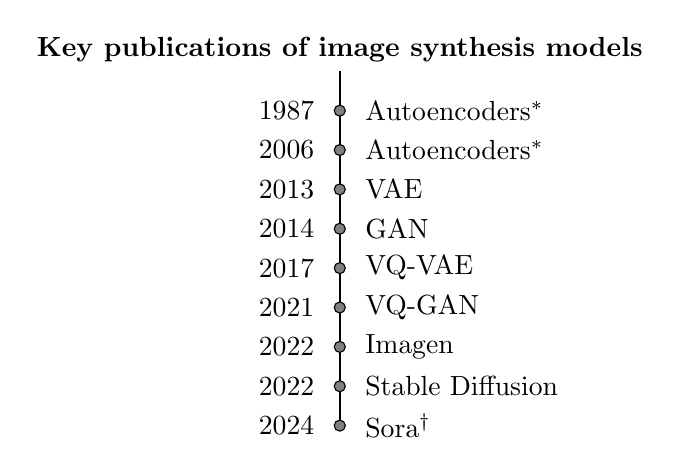
\begin{tikzpicture}
        \def\step{0.5} % step size for vertical spacing
        \def\numtimeline{9} % Number of events in the timeline

        % Define timeline line
        \draw[thick, color=black] (0,0) -- (0,-\numtimeline*\step);

        % Define timeline events with adjusted positions
        \foreach \i/\year/\text in 
        {
            1/1987/Autoencoders$^*$, 
            2/2006/Autoencoders$^*$, 
            3/2013/VAE, 
            4/2014/GAN, 
            5/2017/VQ-VAE,
            6/2021/VQ-GAN,
            7/2022/Imagen,
            8/2022/Stable Diffusion,
            9/2024/Sora$^\dag$
        } {
        \draw[fill=darkgray] (0,-\i*\step) circle (2pt);
        \node[anchor=east] at (-0.2,-\i*\step) {\year};
        \node[anchor=west] at (0.2,-\i*\step) {\text};
        }

        % Define timeline title
        \node[anchor=south] at (0,0) {\textbf{Key publications of image synthesis models}};
    \end{tikzpicture}
    \caption{Chronology of key image generation models publications $^*$The earliest mention of autoencoders appears in an 1986 publication \cite{autoencoder_original_paper_1986}, however the model was not widely used until 2006 when Hinton published a paper that uses autoencoders for dimensionality reduction \cite{autoencoder_2006_paper} which sparked interest in the model again.$^\dag$Although Sora \cite{sora_website} is not specifically an image generation model, it is considered a significant advancement in video synthesis field, which largely relies on image generation.}
    \label{fig:timeline}
  \end{figure}

\subsection{Mathematical Formulation of Generative Models}
Mathematically speaking, let $x$ be a random variable representing a single data point (e.g. an image) of a dataset ${x_1,x_2,...,x_n}$. And let $p(x)$ denote the true probability density function (PDF) of the dataset. Then our objective (as in generative modeling) is to learn a function $q(x;\theta)$ that approximates the true data distribution $p(x)$ (where $\theta$ is the model's parameters). The goal is to estimate $p(x)$ such that new samples $\hat{x} \in p(x)$ drawn from this distribution resemble the dataset.

Most of the time, it is infeasible to calculate directly $p(x)$ because computing the exact probability density for high-dimensional data is computationally expensive and often requires integrating over a large number of variables. This complexity leads to intractable calculations, making it difficult to directly model $p(x)$. Instead, we use various techniques to approximate it, and we denote it as: $q(x;\theta) \sim p(x)$.

\subsection{Approximating the Data Distribution}

In order to approximate $p(x)$ we can use a generative model, where the training objective is to learn the parameters $\theta$ of the model. The success or failure of the model to correctly approximate the dataset distribution can be evaluated using different loss functions, such as maximizing likelihood functions (Appendix \ref{appendix:likelihood_function}), minimizing Kullback-Leibler (KL) divergence, or using adversarial training loss (in the case of GANs).

\subsection{Sampling}

Once trained, the generative model can be used to generate new samples $\hat{x} \sim q(x;\theta)$. Sampling data point $\hat{x}$ will be consistent with the patterns and characteristics of the original dataset, as the model has learned to approximate the true data distribution. Each model will have different strategies to sample. For example, in GANs a random noise vector is sampled from a normal distribution and passed through the generator to generate a new sample, and in VQ-GAN a transformer is used to generate latent codes that are then passed through the decoder to generate an image.

\subsection{Evaluation metrics}

Evaluation of the trained model is done using metrics such as sample quality, diversity (variety in generated samples), and coverage (how well the model covers the data distribution). As we will find later, one of the main problems of the GAN model is called 'mode collapse' \ref{gan_mode_collapse} which causes instability of the model during training, which is manifested in large fluctuations in the loss function or in the fact that the generator fails to converge to an optimal solution that represents the entire distribution of training data. In other words, the model's output isn't diverse enough and only focuses on specific modes of the data distribution (e.g. generating only one type of image, like a cat, whereas the dataset is a collection of all animals).





\textbf{Inception Score.} One of the most common metrics used to evaluate the quality of generated samples is the Inception Score (IS) \cite{is_score}. The IS metric measures the quality and diversity of the generated samples. A good generative model should not only produce images that look visually realistic but also capture the underlying statistical properties of the dataset. A high IS score indicates that the generated samples are both realistic and diverse. IS uses pre-trained Inception V3 model \cite{inception_v3_model} to extract features and classify images to labels. The Inception V3 model is made of multiple convolutional layers and pooling layers and the last layers are fully connected layers with softmax activation function (output is probability of labels) that output the class labels (1000 classes). Two generative models are compared to each other with IS by running the same Inception V3 model, and comparing their scores relatively. The IS is calculated by first computing the conditional entropy of the generated samples given the class label: 

\[
    p(y) = \frac{1}{N} \sum_{i=1}^{N} p(y|x_i)
\] 

(where $y$ is the class label and $x$ is an image, $p(y|x)$ is the conditional probability of the label $y$ given image $x$) (i.e., the diversity of generated samples) and then computing the \textbf{KL divergence} between the marginal distribution of the generated samples and the conditional distribution:

\[
    D_{\text{KL}}(p(y|x) \| p(y)) = \sum_{y} p(y|x) \log \frac{p(y|x)}{p(y)}
\]

(where $p(y)$ is the marginal probability of the label across the set of generated images, and $D_{KL}$ is the Kullback-Leibler (KL) divergence between the conditional label distribution $p(y|x)$ and marginal label distribution $p(y)$). Finally, we get the IS score as:

\[
    \text{IS} = \exp \left( \frac{1}{N} \sum_{i=1}^{N} D_{\text{KL}}(p(y|x_i) \| p(y)) \right) = \exp(\mathbb{E}_{x \sim p_g} \left[ D_{\text{KL}} \left( p(y | x) \Vert p(y) \right) \right])
\]

Where $p_g$ is the distribution of the generated images. The IS score is the exponential of the sum of these two terms. A high IS score indicate that the generated samples are both realistic and diverse because $p(y|x)$ should be sharp (i.e. indicating generated samples are high quality), and $p(y)$ should be uniform (i.e. generated samples are diverse).






\textbf{FID Score.} Frechet Inception Distance (FID) score \cite{fid_score} is an improvement on the Inception Score and is more recent. The FID score also measures the similarity between the generated samples and the real data distribution, and the diversity. FID aims to capture this by comparing the feature distributions, not just individual image similarity. The lower the FID score, the better the model is at generating samples that resemble the real data distribution. FID leverages a pre-trained image classification model (which is also typically Inception V3 model), to extract high-level features from both the generated images and the dataset. These features capture the essential characteristics of the images, like shapes, textures, and object relationships. Then, its possible to compare generative models based on the similarity of these features relatively to the same dataset, compared to just looking at the labels in Inception Score. The FID score is calculated as:

\begin{equation}
    \text{FID} = ||\mu_x - \mu_g||^2 + Tr(\Sigma_x + \Sigma_g - 2(\Sigma_x\Sigma_g)^{1/2})
    \label{eq:fid_score}
\end{equation}

where $\mu_x$ and $\Sigma_x$ are the mean and covariance of the feature distribution of the dataset, and $\mu_g$ and $\Sigma_g$ are the mean and covariance of the feature distribution of the generated images. The FID score is the Euclidean distance between the means and the trace (matrix operation) of the covariance matrices. A lower FID score indicates that the generated samples are more similar to the real data distribution.


\section{Variational Autoencoder}
\label{sec:vae}

Variational Autoencoder (VAE) \cite{vae} is generative model is used to learn the underlying distribution of data and generate new samples (similar to the dataset). The model consists of 3 main components: an encoder, latent space (sometimes called 'code vectors' or 'bottleneck layer') and a decoder. The main idea behind VAE is to use the autoencoder model \cite{autoencoder} \cite{autoencoder2} to compress large dimensional vectors (in our case, images) into smaller, low dimension vectors that represent the underlying features hidden within the input data. These code vectors are then fed into a decoder network which reconstructs the image (i.e. high dimensional vector).


\begin{figure}[h]
    \centering
    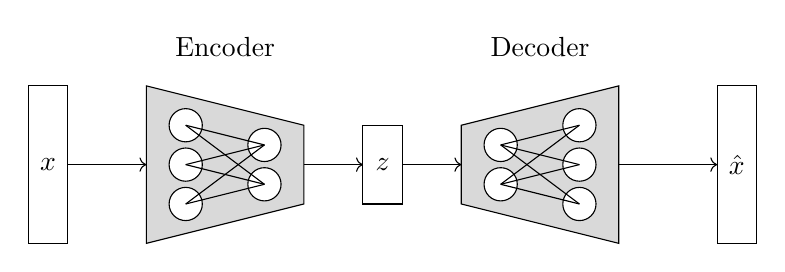
\begin{tikzpicture}
        % Center point of encoder
        \coordinate (E_CENTER) at (1, 1);
        \coordinate (INPUT_TEXT) at (-0.25, 0.5);



        % Draw input vector
        \draw ($(INPUT_TEXT) + (-0.25, -0.5)$) rectangle ($(INPUT_TEXT) + (0.25, 1.5)$) node[pos=.5] {$x$};
        \draw[->] ($(E_CENTER) + (-1, 0)$) -- (E_CENTER);

        








        % Draw the encoder
        \node at ($(E_CENTER) + (1, 1.5)$) {Encoder};
        
        \coordinate (A) at ($(E_CENTER) + (0, -1)$);
        \coordinate (B) at ($(E_CENTER) + (2, -0.5)$);
        \coordinate (C) at ($(E_CENTER) + (2, 0.5)$);
        \coordinate (D) at ($(E_CENTER) + (0, 1)$);
        \draw[fill=gray!30] (A) -- (B) -- (C) -- (D) -- cycle;
        
        % Define the coordinates for the first set of circles (3 neurons)
        \coordinate (n1) at ($(E_CENTER) + (0.5, -0.5)$);
        \coordinate (n2) at ($(E_CENTER) + (0.5, 0)$);
        \coordinate (n3) at ($(E_CENTER) + (0.5, 0.5)$);
        
        % Define the coordinates for the second set of circles (2 neurons)
        \coordinate (m1) at ($(E_CENTER) + (1.5, 0.25)$);
        \coordinate (m2) at ($(E_CENTER) + (1.5, -0.25)$);
        
        % Draw the first set of circles
        \foreach \i in {n1, n2, n3} {
            \filldraw[fill=white] (\i) circle (6pt);
        }
        
        % Draw the second set of circles
        \foreach \i in {m1, m2} {
            \filldraw[fill=white] (\i) circle (6pt);
        }
        
        % Draw arrows from each circle in the first set to each circle in the second set
        \foreach \i in {n1, n2, n3} {
            \foreach \j in {m1, m2} {
                \draw[-] (\i) -- (\j);
            }
        }






        % Draw code vector

        % Arrow in
        \coordinate (Z_TEXT) at ($(E_CENTER) + (3, 0)$);
        \draw[->] ($(E_CENTER) + (2, 0)$) -- ($(Z_TEXT) + (-0.25, 0)$);

        \draw ($(Z_TEXT) + (-0.25, -0.5)$) rectangle ($(Z_TEXT) + (0.25, 0.5)$) node[pos=.5] {$z$};
        
        % Arrow out
        \coordinate (D_CENTER) at ($(E_CENTER) + (4, 0)$);
        \draw[->] ($(Z_TEXT) + (0.25, 0)$) -- (D_CENTER);











        % Draw decoder
        \node at ($(D_CENTER) + (1, 1.5)$) {Decoder};
        
        \coordinate (A2) at ($(D_CENTER) + (0, 0.5)$);
        \coordinate (B2) at ($(D_CENTER) + (2, 1)$);
        \coordinate (C2) at ($(D_CENTER) + (2, -1)$);
        \coordinate (D2) at ($(D_CENTER) + (0, -0.5)$);
        \draw[fill=gray!30] (A2) -- (B2) -- (C2) -- (D2) -- cycle;
        
        % Define the coordinates for the first set of circles (2 neurons)
        \coordinate (n2_1) at ($(D_CENTER) + (0.5, 0.25)$);
        \coordinate (n2_2) at ($(D_CENTER) + (0.5, -0.25)$);
        
        % Define the coordinates for the second set of circles (3 neurons)
        % \coordinate (m2_1) at (1.5, 0.5);
        % \coordinate (m2_2) at (1.5, 1);
        % \coordinate (m2_3) at (1.5, 1.5);
        \coordinate (m2_1) at ($(n2_1) + (1, 0.25)$);
        \coordinate (m2_2) at ($(n2_1) + (1, -0.25)$);
        \coordinate (m2_3) at ($(n2_1) + (1, -0.75)$);
        
        % Draw the first set of circles
        \foreach \i in {n2_1, n2_2} {
            \filldraw[fill=white] (\i) circle (6pt);
        }
        
        % Draw the second set of circles
        \foreach \i in {m2_1, m2_2, m2_3} {
            \filldraw[fill=white] (\i) circle (6pt);
        }
        
        % Draw arrows from each circle in the first set to each circle in the second set
        \foreach \i in {n2_1, n2_2} {
            \foreach \j in {m2_1, m2_2, m2_3} {
                \draw[-] (\i) -- (\j);
            }
        }


        \coordinate (D_END) at ($(D_CENTER) + (2, 0)$);




        % Draw output vector
        \coordinate (X_OUT_TEXT) at ($(m2_2) + (2, 0)$);
        \draw[->] (D_END) -- ($(X_OUT_TEXT) + (-0.25, 0)$);
        
        \draw ($(X_OUT_TEXT) + (-0.25, -1)$) rectangle ($(X_OUT_TEXT) + (0.25, 1)$) node[pos=.5] {$\hat{x}$};
        
        % \node at (X_OUT_TEXT) {$\hat{x}$};
        
    \end{tikzpicture}
    \caption{Autoencoder architecture.}
\end{figure}


More formally, the encoder network takes an input data point $x$ and maps it to a latent space representation $z$, which is compressed representation of $x$. The input is a vector, therefor an image must be flattened from 2D to 1D vector. This flattening will become an issue later in image generation, as this action removes important spatial information and hidden structures in the image. Because of this, modifications were made to the VAE model which allows the capture of spatial information by using a CNN (Convolutional Neural Network) \cite{cnn} layers \cite{vae_cnn_example}, max pooling layers, and more. After compression, the latent vector $z$ is then passed onto the decoder for reconstruction. 

The reconstruction is learned by a reconstruction loss function, usually mean squared error (MSE) loss function:

\begin{equation}
    \text{MSE} = \frac{1}{N} \sum_{i=1}^{N} (y_i - \hat{y}_i)^2
\label{eq:mse}
\end{equation}

The MSE loss is common in image generation models, because this loss is used to ensure that the generated images closely resemble the original input images by comparing the distance between pixels (input image, output image). This objective motivates the model to reconstruct the image from latent vector to resemble the original image. However, this loss is not used alone usually, but in combination with more complex loss functions, as we will see later in VAE.

The code vectors learned by autoencoders, however, are one-to-one map of the input and code vector (deterministic mapping from input to code vectors). The model doesn't capture any semantic relationships between the data (e.g the code vectors of images of cats are scattered throughout the entire latent space, whereas in VAE, they are clustered together). The latent space in autoencoders is irregular and discontinuous, meaning a small change in the latent vector can lead to large unpredictable changes in the output. This makes interpolation in the latent space difficult. Variational autonecoder solve this problem. VAE regularizes the latent space by enforcing a prior distribution. This regularization leads to a smooth and continuous latent space (see figure \ref{fig:ae_vs_vae}), which allows the model to interpolate between the latent space smoothly, thus creating similar new images with different variations. VAEs also provide an explicit model of the data distribution by maximizing a variational lower bound on the likelihood of the data. In other words, VAE is probabilistic model instead of discrete mapper (like the autoencoder model).

\begin{figure}[h]
    \centering
    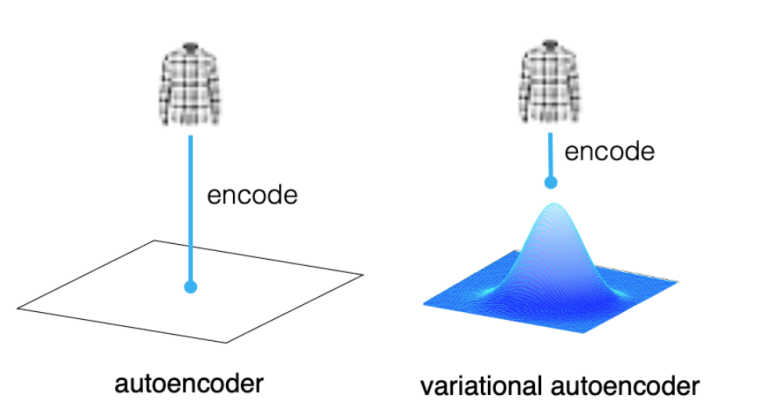
\includegraphics[scale=0.5]{images/autoencoder-vs-variational-autoencoder-point-vs-distribution-768x409.png}
    \caption{Illustration of mapping an input image to code vector (left) and mapping an input image to a distribution (right) \cite{ae_vs_vae}.}
    \label{fig:ae_vs_vae}
\end{figure}

At the heart of VAE lies the concept of latent variables (Appendix \ref{appendix:latent_variables}). Latent variables are hidden, unobserved variables that the model infers from the observed data (dataset). Latent variable models, such as VAE, take indirect approach to describing a probability distribution $p(x)$ over multi-dimensional variable $x$. Instead of directly writing the expression for $p(x)$, they model a joint distribution $p(x|z)$ of the data $x$ and an unobserved hidden latent variable $z$.

The variational aspect of VAE refers to the use of variational inference (VI) (Appendix \ref{appendix:variational_inference}). VI is used to used to approximate complex posterior distributions: 

\begin{equation}
p(z|x) = \frac{p(x|z) \cdot p(z)}{\int p(x|z) \cdot p(z) dz}
\label{eq:posterior}
\end{equation}

by transforming the problem into optimization problem. The denominator in eq. \ref{eq:posterior} is intractable because it involves integrating over all possible values of $z$, and $z$ is often relatively high-dimensional and its infeasible to evaluate exactly. Which is why VI is used, which approximates the true posterior distribution $p(z|x)$ with simpler, tractable distribution $q_\phi (z|x)$, parameterized by $\phi$.

The original VAE model uses fully connected layers at the encoder and decoder networks. However, in the image synthesis field, CNN layers (appendix \ref{appendix:cnn}) are used instead which are computationally less expensive and better capture the spatial information, for instance, its used in VQ-VAE (section \ref{sec:vqvae}) and PixelCNN \cite{pixelcnn}.

To generate an image, we first sample a latent variable $z$ from prior distribution $p(z)$, which is typically standard normal distribution $\mathcal{N}(0, 1)$. Then $z$ is passed to the decoder an an image $x$ is generated from the conditional distribution $p_\theta (x|z)$. 

\subsection{The Reparameterization Trick}
To enable backpropagation through the sampling process, VAEs use the reparameterization trick. This trick involves expressing the sampled latent variables $z$ as a deterministic function of the encoder's output and some random noise. Without this technique, backpropagation would not be possible through the sampling operation. The reason is that sampling is a non-differentiable operation, because sampling from a distribution involves randomness that does not have a gradient, and the gradients cannot be computed with respect to the parameters of the encoder. To make the sampling operation differentiable and thus allow gradients to flow through the network, the reparameterization trick is used. 

Specifically, if $\mu$ and $\sigma$ are the mean and standard deviation vectors outputted by the encoder, we can write:

\begin{equation}
    z = \mu + \sigma \cdot \epsilon
\end{equation}

where $\epsilon \sim \mathcal{N}(0, 1)$ is a standard normal random variable. This $\epsilon$ will not change throughout the training reigime. It is sampled once and fixed in place. This trick allows us instead of having full stochastic node that blocks flow of gradients, to having two parts: one where we can do backpropagation, and another part which is still stochastic but which we don't want to train because its fixed.


\begin{figure}[h]
    \centering
    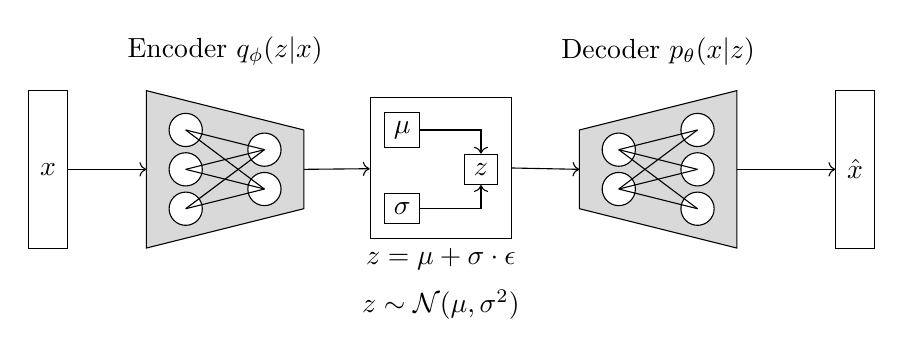
\begin{tikzpicture}
        % Center point of encoder
        \coordinate (E_CENTER) at (1, 1);
        \coordinate (INPUT_TEXT) at (-0.25, 0.5);



        % Draw input vector
        \draw ($(INPUT_TEXT) + (-0.25, -0.5)$) rectangle ($(INPUT_TEXT) + (0.25, 1.5)$) node[pos=.5] {$x$};
        \draw[->] ($(E_CENTER) + (-1, 0)$) -- (E_CENTER);

        








        % Draw the encoder
        \node at ($(E_CENTER) + (1, 1.5)$) {Encoder $q_\phi(z|x)$};
        
        \coordinate (A) at ($(E_CENTER) + (0, -1)$);
        \coordinate (B) at ($(E_CENTER) + (2, -0.5)$);
        \coordinate (C) at ($(E_CENTER) + (2, 0.5)$);
        \coordinate (D) at ($(E_CENTER) + (0, 1)$);
        \draw[fill=gray!30] (A) -- (B) -- (C) -- (D) -- cycle;
        
        % Define the coordinates for the first set of circles (3 neurons)
        \coordinate (n1) at ($(E_CENTER) + (0.5, -0.5)$);
        \coordinate (n2) at ($(E_CENTER) + (0.5, 0)$);
        \coordinate (n3) at ($(E_CENTER) + (0.5, 0.5)$);
        
        % Define the coordinates for the second set of circles (2 neurons)
        \coordinate (m1) at ($(E_CENTER) + (1.5, 0.25)$);
        \coordinate (m2) at ($(E_CENTER) + (1.5, -0.25)$);
        
        % Draw the first set of circles
        \foreach \i in {n1, n2, n3} {
            \filldraw[fill=white] (\i) circle (6pt);
        }
        
        % Draw the second set of circles
        \foreach \i in {m1, m2} {
            \filldraw[fill=white] (\i) circle (6pt);
        }
        
        % Draw arrows from each circle in the first set to each circle in the second set
        \foreach \i in {n1, n2, n3} {
            \foreach \j in {m1, m2} {
                \draw[-] (\i) -- (\j);
            }
        }






        % Draw middle
        \coordinate (Z_TEXT) at ($(E_CENTER) + (3, 0)$);

        \coordinate (MIDDLE_BEGIN) at ($(Z_TEXT) + (-0.5, 0)$);
        \coordinate (MU_BEGIN) at ($(MIDDLE_BEGIN) + (0.25, 0.5)$);
        \coordinate (SIGMA_BEGIN) at ($(MIDDLE_BEGIN) + (0.25, -0.5)$);
        \coordinate (Z_BEGIN) at ($(Z_TEXT) + (0.75, 0)$);

        \coordinate (ARROW_OUT_BEGIN) at ($(Z_TEXT) + (1.75, 0)$);
        \coordinate (ARROW_OUT_END) at ($(ARROW_OUT_BEGIN) + (0.5, 0)$);

        % Middle nodes
        \node[draw,rectangle] (SIGMA) at ($(SIGMA_BEGIN) + (0.5, 0)$) {$\sigma$};
        \node[draw,rectangle] (MU) at ($(MU_BEGIN) + (0.5, 0)$) {$\mu$};
        \node[draw,rectangle] (Z) at ($(Z_BEGIN) + (0.5, 0)$) {$z$};

        % Rectangle around all nodes
        \node[draw, rectangle, inner sep=5pt, fit=(SIGMA) (MU) (Z)] (middle_rect) {};

        % Equations below the rectangle
        \node[below=0cm of middle_rect] (eq1) {$z = \mu + \sigma \cdot \epsilon$};
        \node[below=0cm of eq1] (eq2) {$z \sim \mathcal{N}(\mu, \sigma^2)$};

        % Arrow from trapazoid to rectangle
        \draw[->] ($(E_CENTER) + (2, 0)$) -- (middle_rect);

        % Inner arrows
        \draw[->, to path={-| (\tikztotarget)}] (SIGMA) edge (Z) (MU) edge (Z);











        % Draw decoder
        \coordinate (D_CENTER) at ($(Z_TEXT) + (2.5, 0)$);
        \node at ($(D_CENTER) + (1, 1.5)$) {Decoder $p_\theta(x|z)$};

        % Arrow from the rectangle to the trapezoid
        \draw[->] (middle_rect.east) -- (D_CENTER);

        % Draw trapazoid
        \coordinate (A2) at ($(D_CENTER) + (0, 0.5)$);
        \coordinate (B2) at ($(D_CENTER) + (2, 1)$);
        \coordinate (C2) at ($(D_CENTER) + (2, -1)$);
        \coordinate (D2) at ($(D_CENTER) + (0, -0.5)$);
        \draw[fill=gray!30] (A2) -- (B2) -- (C2) -- (D2) -- cycle;
        
        % Define the coordinates for the first set of circles (2 neurons)
        \coordinate (n2_1) at ($(D_CENTER) + (0.5, 0.25)$);
        \coordinate (n2_2) at ($(D_CENTER) + (0.5, -0.25)$);
        
        % Define the coordinates for the second set of circles (3 neurons)
        \coordinate (m2_1) at ($(n2_1) + (1, 0.25)$);
        \coordinate (m2_2) at ($(n2_1) + (1, -0.25)$);
        \coordinate (m2_3) at ($(n2_1) + (1, -0.75)$);
        
        % Draw the first set of circles
        \foreach \i in {n2_1, n2_2} {
            \filldraw[fill=white] (\i) circle (6pt);
        }
        
        % Draw the second set of circles
        \foreach \i in {m2_1, m2_2, m2_3} {
            \filldraw[fill=white] (\i) circle (6pt);
        }
        
        % Draw arrows from each circle in the first set to each circle in the second set
        \foreach \i in {n2_1, n2_2} {
            \foreach \j in {m2_1, m2_2, m2_3} {
                \draw[-] (\i) -- (\j);
            }
        }


        \coordinate (D_END) at ($(D_CENTER) + (2, 0)$);

        % Draw output vector
        \coordinate (X_OUT_TEXT) at ($(m2_2) + (2, 0)$);
        \draw[->] (D_END) -- ($(X_OUT_TEXT) + (-0.25, 0)$);
        
        \draw ($(X_OUT_TEXT) + (-0.25, -1)$) rectangle ($(X_OUT_TEXT) + (0.25, 1)$) node[pos=.5] {$\hat{x}$};
        
        % \node at (X_OUT_TEXT) {$\hat{x}$};
        
    \end{tikzpicture}
    \caption{Variational Autoencoder architecture.}
    \label{figure:vae}
\end{figure}


The VAE architecture is shown in figure \ref{figure:vae}.

\subsection{Training}

The VAE optimizes the Evidence Lower Bound (ELBO) (see appendix \ref{appendix:elbo}) to ensure that the approximate posterior $q_\phi (z|x)$ is close to the true posterior $p(z|x)$ (we want to maximize it):

\begin{equation}
    \mathcal{L}(\theta, \phi; x, z) = \text{ELBO} = \mathbb{E}_{q_\phi(z|x)} \left[ \log p_\theta(x|z) \right] - D_\text{KL}(q_\phi(z|x) \| p(z))
\end{equation}

where the first term is the reconstruction loss and the second term is the KL divergence (see appendix \ref{appendix:kl_divergence}) (which measure how much the approximate posterior $q_\phi (z|x)$ diverges from the prior $p(z)$). 
\section{VQ-VAE}
\label{sec:vqvae}

Vector Quantized Variational Autoencoder (VQ-VAE) \cite{vqvae} is a generative models based on VAE \ref{sec:vae} model with the addition of vector quantization (VQ) (section \ref{subsec:vqvae_vq}) technique. 

\subsection{Vector Quantization}
\label{subsec:vqvae_vq}

Vector quantization (VQ) is a technique used to discretize continuous data. In the context of VQ-VAE, the continuous latent space $z$ is mapped into discrete codes vectors. In a continuous latent space, the amount of possibilities for a value in the hidden space is infinite, which makes it difficult for the model to learn the hidden space efficiently. With a discrete hidden space, learning becomes more efficient because there is a fixed number of possible values (although in reality it is very large, for example the amount of objects that can be described using language is finite but very large). Furthermore, in reality, images are divided into classes of objects such as cats, people, dogs, etc., and each class has a finite number of possibilities, which is better suited to a discrete latent vectors.

\begin{figure}[h]
    \centering
    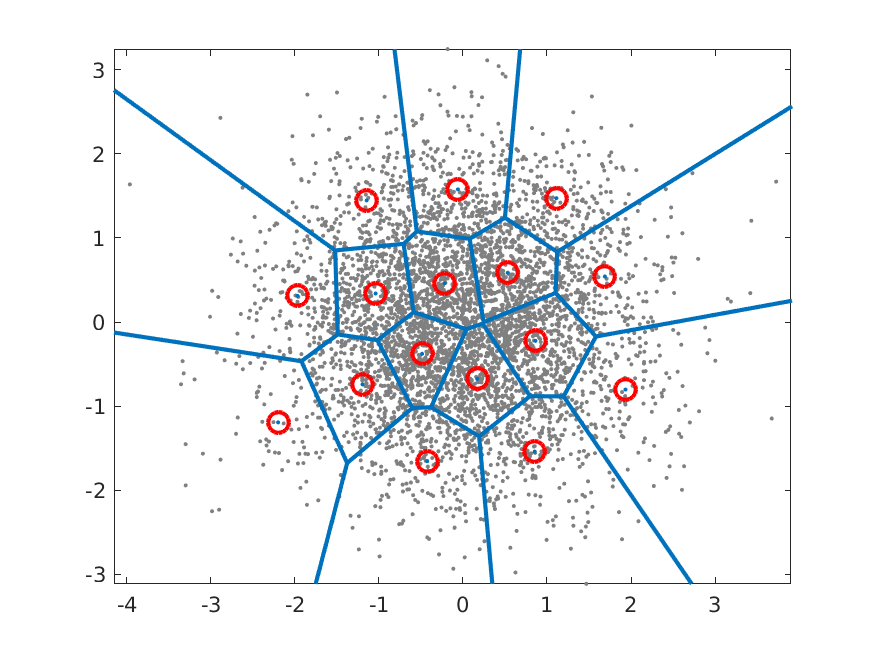
\includegraphics[scale=0.5]{images/vq_visualization.png}
    \caption{Illustration of vector quantization discrete clustering of the 2D latent space \cite{vq_visualization_website}. The grey dots are embeddings of the continous latent space, and the red dots are the code vectors from the codebook. In this case, the codebook size is 16.}
    \label{figure:vq_visualization}
\end{figure}

This technique involves the use of a codebook, which is a discrete collection of vectors of the same size as the hidden dimension. In the VQ-VAE model, after the input passes through the encoder (which results in embeddings - which are the hidden representation of the input), the embeddings are replaced by the closest vector from the codebook (by minimizing distance between vectors). This operation allows the model to learn clusters of similar embeddings, which can be used to generate new samples. The codebook is learned during training, and the embeddings are quantized to the nearest code vector in the codebook. The codebook is learned by minimizing the loss function:

\begin{equation}
    \mathcal{L}_{\text{VQ}} = || \text{sg}[z_e] - z_q ||_2^2 + \beta || \text{sg}[z_q] - z_e ||_2^2
\label{eq:vq_loss}
\end{equation}

where $z_e$ is the encoder output, $z_q$ is the quantized output, $\text{sg}[\cdot]$ is the stop gradient operation (which prevents gradients from flowing through the quantization operation), and $\beta$ is a hyperparameter that controls the weighting of the two terms in the loss function. The first term in the loss function is the quantization loss, which measures the distance between the encoder output and the quantized output. The second term is the commitment loss, which measures the distance between the quantized output and the encoder output. The commitment loss encourages the model to use the codebook, and prevents the model from ignoring the quantization operation.

\subsection*{Architecture}

ABC

\subsection*{Training}

ABC
\section{Generative Adversarial Networks (GANs)}
\label{sec:gan}

\begin{figure}
    \centering
    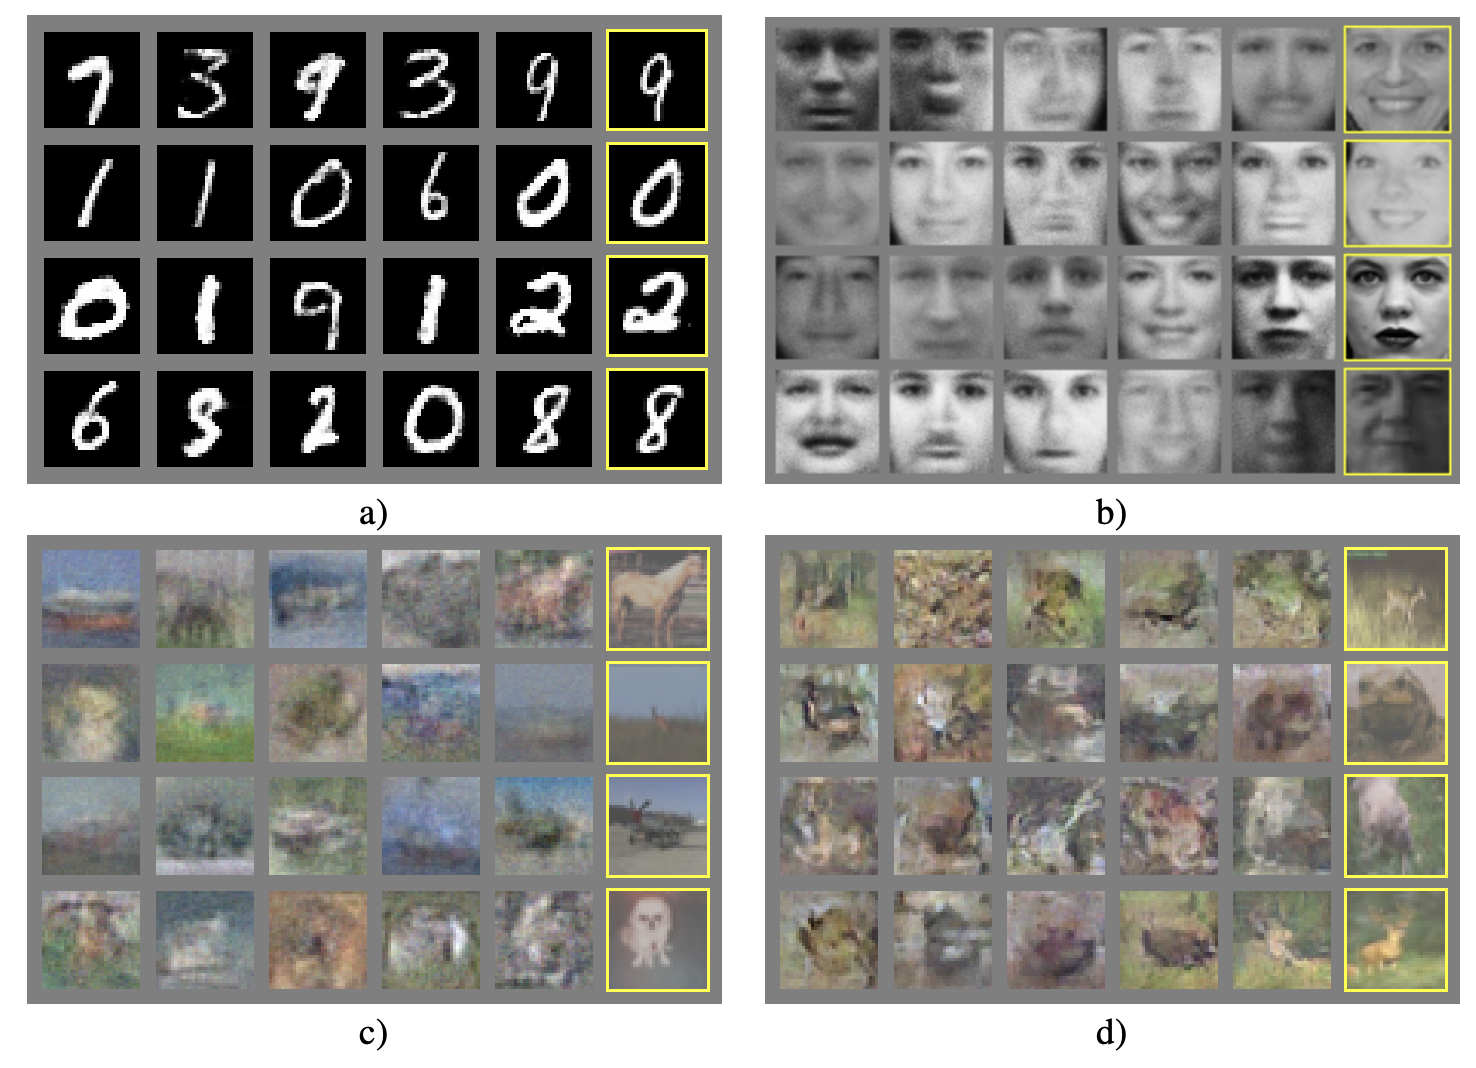
\includegraphics[width=0.75\textwidth]{images/gan_samples.png}
    \caption{Some samples generated by GAN in the paper \cite{gan}. Right: samples from the training data. Left: samples generated by the model. a) is from the MNIST dataset, b) is from the Toronto Face Database (TFD), c) is from the CIFAR-10 dataset with fully-connected layers at the generator and discriminator, and d) is from the CIFAR-10 dataset with convolutional layers at the generator and discriminator.}
\end{figure}

Generative Adversarial Networks (GANs) \cite{gan} are a class of deep learning models that are used to generate new data samples from a given distribution. More specifically, they are very good at synthesizing high-quality images. The model can be used by itself, or as we will see later, it can also be the basis of other image and video generation models, such as VQ-GAN \ref{sec:vqgan}.

\begin{figure}
    \centering
    \resizebox{\textwidth}{!}{
        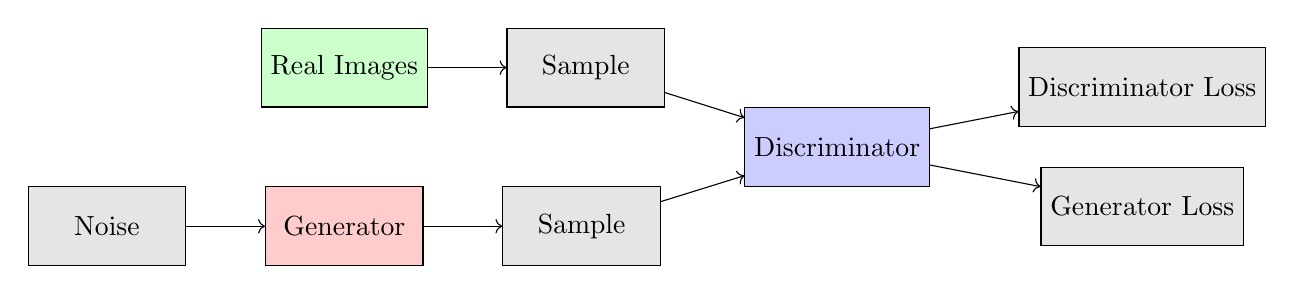
\begin{tikzpicture}
            % Real images, Generator nodes
            \node[rectangle, draw, fill=green!20, minimum width=2cm, minimum height=1cm] (real_images) {Real Images};
            \node[rectangle, draw, fill=red!20, minimum width=2cm, minimum height=1cm, below=of real_images] (generator) {Generator};

            % Noise node
            \node[rectangle, draw, fill=gray!20, minimum width=2cm, minimum height=1cm, left=of generator] (noise) {Noise};

            % Arrow from noise to generator
            \draw[->] (noise) -- (generator);

            % Sample nodes
            \node[rectangle, draw, fill=gray!20, minimum width=2cm, minimum height=1cm, right=of generator] (sample_gen) {Sample};
            \node[rectangle, draw, fill=gray!20, minimum width=2cm, minimum height=1cm, right=of real_images] (sample_real_images) {Sample};

            % Fit sample nodes in a box
            \node[fit=(sample_gen)(sample_real_images), inner sep=0] (sample_fitbox) {};


            % Arrows to sample nodes
            \draw[->] (real_images) -- (sample_real_images);
            \draw[->] (generator) -- (sample_gen);

            % Discriminator node
            \node[rectangle, draw, fill=blue!20, minimum width=2cm, minimum height=1cm, right=of sample_fitbox] (discriminator) {Discriminator};

            % Arrows to discriminator
            \draw[->] (sample_real_images) -- (discriminator);
            \draw[->] (sample_gen) -- (discriminator);

            % Discriminator loss, Generator loss
            % Matrix for the nodes to the right
            \matrix[
                right=of discriminator, 
                column sep=0.5cm, 
                row sep=0.5cm, 
                nodes={rectangle, draw, minimum width=4cm, minimum height=2cm, anchor=center}
            ] (matrix) {
                \node[rectangle, draw, fill=gray!20, minimum width=2cm, minimum height=1cm] (discriminator_loss) {Discriminator Loss}; \\
                \node[rectangle, draw, fill=gray!20, minimum width=2cm, minimum height=1cm] (generator_loss) {Generator Loss}; \\
            };

            % Add arrows
            \draw[->] (discriminator) -- (discriminator_loss);
            \draw[->] (discriminator) -- (generator_loss);
        \end{tikzpicture}
    }
    \caption{GAN architecutre \cite{gan}. Noise is sampled from a noise distribution and fed to the generator. The generator outputs an image, and the discriminator needs to decide if the image was generated by the generator or if its an image from the dataset. This decision then affects the value of the loss function, and the weights are updated accordingly by backpropogation.}
    \label{fig:gan_architecture}
\end{figure}

% TODO: \ref{fig:gan_architecture} is referencing to the GAN section, and not the figure! WTF
The model consists of two neural networks: a generator $G$ and a discriminator $D$ (as shown in figure \ref{fig:gan_architecture}). The generator is responsible for generating new samples $x$ (images), while the discriminator is responsible for distinguishing between real samples (from the dataset, $D(x) = 1$) and generated samples (fake, from the generator, $D(x) = 0$). The two networks are trained simultaneously in a minimax game (see training section \ref{subsec:gan_training}), where the generator tries to generate samples that are indistinguishable from real samples, and the discriminator tries to distinguish between real and generated samples. The training process continues until the generator is able to generate realistic and high-quality images. 

The noise vector is sampled from a simple distribution like Gaussian. The basic idea of using noise as input is that the model learns to establish relationships between each dimension in the vector and the output image, similar to latent vectors or code vectors. For instance, the model might learn that the first dimension of the noise vector corresponds to the shape of the middle of the image (like the shape of the head of a person), while the second dimension might corresponds to the color of the shape, and so on.




\subsection{Training}
\label{subsec:gan_training}

The loss function of the GAN model is defined as the following min-max game:

\begin{equation}
    \label{eq:gan_loss}
    \min_G \max_D V(D,G) = \mathbb{E}_{x \sim p_{\text{data}}(x)}[\log D(x)] + \mathbb{E}_{z \sim p_z(z)}[\log(1 - D(G(z)))]
\end{equation}

We have two prior distributions: $x \sim p_{\text{data}}$ and $z \sim p_z(z)$, where the noise vector $z$ is sampled from a noise distribution, and $p_{\text{data}}$ represents the true underlying distribution of the dataset, and $x$ is sampled from this distribution.

With respect to the discriminator gradients, the loss function tries to maximize the probability that:

\begin{enumerate}
    \item the discriminator correctly classifies real samples as real (the first term)
    \item the discriminator correctly classifies generated samples as fake (the second term)
\end{enumerate}


With respect to the generator gradients \footnote{When we do backpropogation with respect to the generatoe gradients, the first term is constant.}, the loss function tries to minimize the probability that:

\begin{enumerate}
    \item the generator tries to fool the discriminator in thinking that the generated samples are real (the second term)
\end{enumerate}


The researchers mentioned that at the beginning of the training, the discriminator rejects samples with high confidense. To address this, they suggested instead of \textbf{minimizing} the second term, to \textbf{maximize} a new second term in the loss function: $\log D(G(z))$.


\begin{figure}
    \centering
    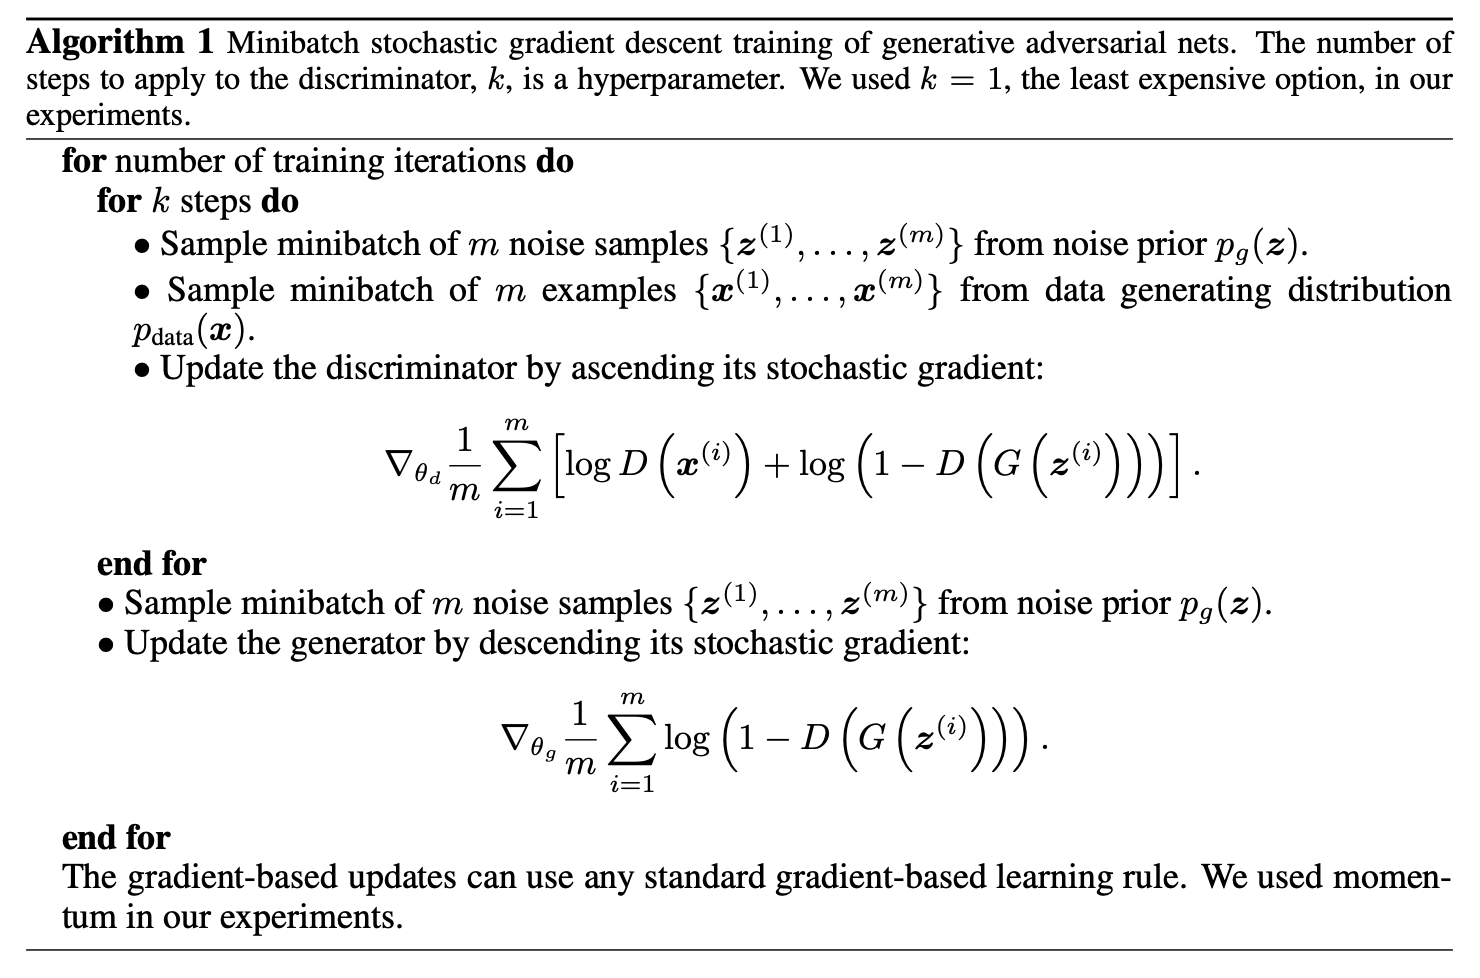
\includegraphics[width=0.75\textwidth]{images/gan_training.png}
    \caption{The training algorithm for GAN using minibatch stochastic gradient decent \cite{gan}.}
    \label{fig:gan_training}
\end{figure}

In order to balance of the training for both $G$ and $D$ the authors suggested using iterative approach using minibatch stochastic gradient decent (see figure \ref{fig:gan_training}). Instead of fully optimizing $D$ in each iteration, the algorithm alternates between a few steps ($k$ steps) of optimizing the discriminator and one step of optimizing the generator. By updating $D$ more often the researchers hope to update the generator more slowly and stabilize the training process.



\subsection{Mode Collapse}

One of the main challenges of training GANs is mode collapse. Mode collapse occurs when the generator learns to generate only a few samples, instead of learning to generate a diverse set of samples. This can happen when the generator learns to generate samples that fool the discriminator, but failed to capture the full diversity of the training data distribution (see figure \ref{fig:gan_mode_collapse}). This can happen when the discriminator is too strong, and the generator is not able to generate diverse samples. In other words, the generator tries to fool the discriminator so much that it only focuses on this goal, while ignoring to diversify the samples.

\begin{figure}
    \centering
    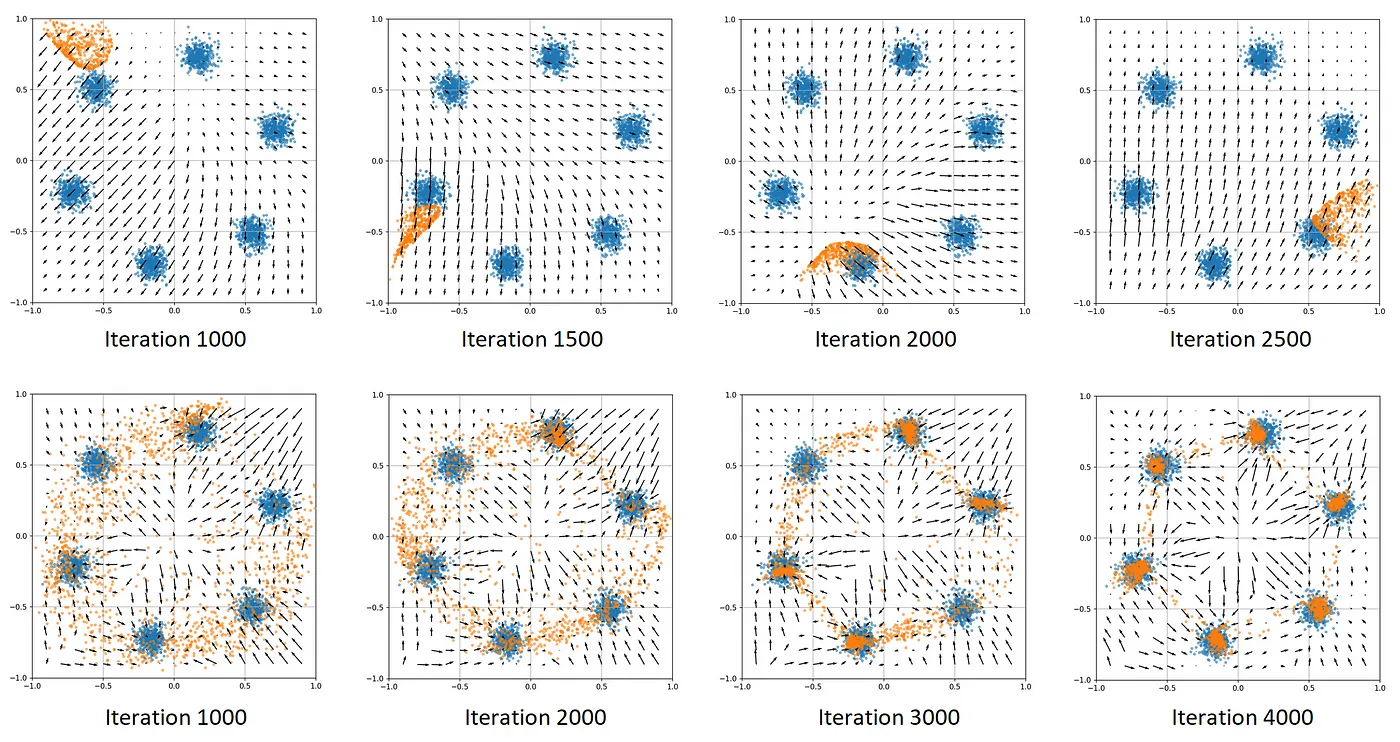
\includegraphics[width=\textwidth]{images/gan_mode_collapse.png}
    \caption{Mode collapse in GANs (top row) \cite{gan_mode_collapse_image_source}. Bottom row shows GAN samples without mode-collapse. Blue dots are the prior $x \sim p_{\text{data}}(x)$ and the orange dots are the generated samples $p_g$.}
    \label{fig:gan_mode_collapse}
\end{figure}

\section{VQ-GAN}
\label{sec:vqgan}

\begin{figure}
    \centering
    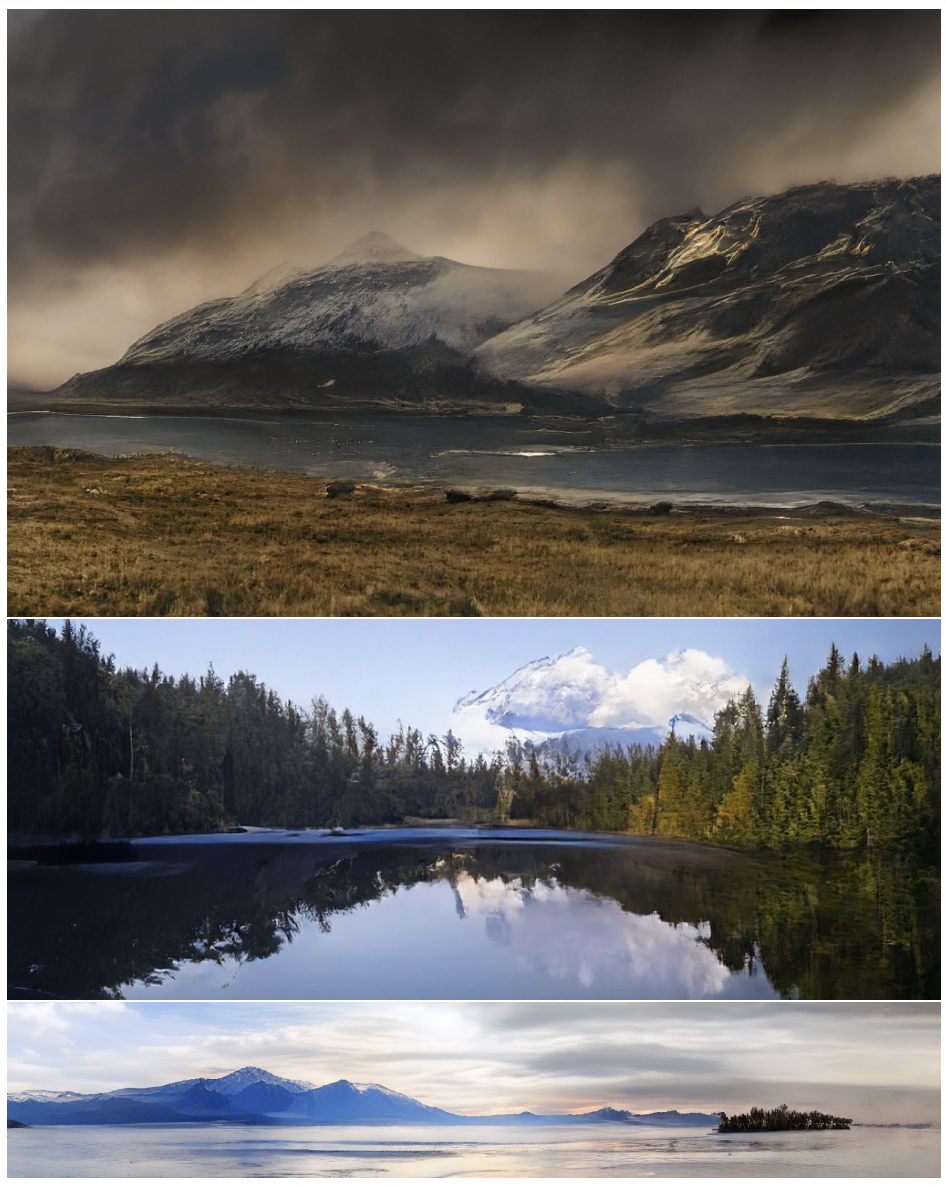
\includegraphics[width=0.5\textwidth]{images/vqgan_samples.png}
    \caption{Samples generated by VQ-GAN with different resolutions (top to bottom: 1280x832, 1024x416, 1280x240), conditioned on semantic layouts from S-FLCKR dataset.}
\end{figure}

Vector Quantized Generative Adversarial Network (VQ-GAN) \cite{vqgan} is a deep learning model capable of generating high-quality images, with the ability of conditioning (text, images, semantic masks and human pose). The architecutre of VQ-GAN is based on previous works: Vector Quantized Variational Autoencoder (VQ-VAE) \cite{vqvae} (section \ref{sec:vqvae}), transformers \cite{transformer} (appendix \ref{appendix:transformers}), and Generative Adversarial Network (GAN) \cite{gan} (section \ref{sec:gan}). The main premises of VQ-GAN is instead of representing an image with pixels, they represent it as a composition of perceptually rich image constituents from a codebook.

VQ-GAN takes the best of both worlds: the ability to generate high-quality images from GANs and the ability to condition the generation process from VQ-VAE using transformers. The combination of the expressivness of transformers and the inductive bias \footnote[1]{Inductive bias is the ability to capture local information in the image, which is why CNN is chosen,  because of the pooling layers.} of CNNs \cite{cnn} in this work showed significant improvements in image generation tasks compared to previous models. Transformers can learn long-range dependencies, whereas CNNs are better fit at learning local features and structures of images. Additional benefit in using a transformer is that is allows the model to output images of various resolutions, which is not possible with previous works.

\begin{figure}
    \centering
    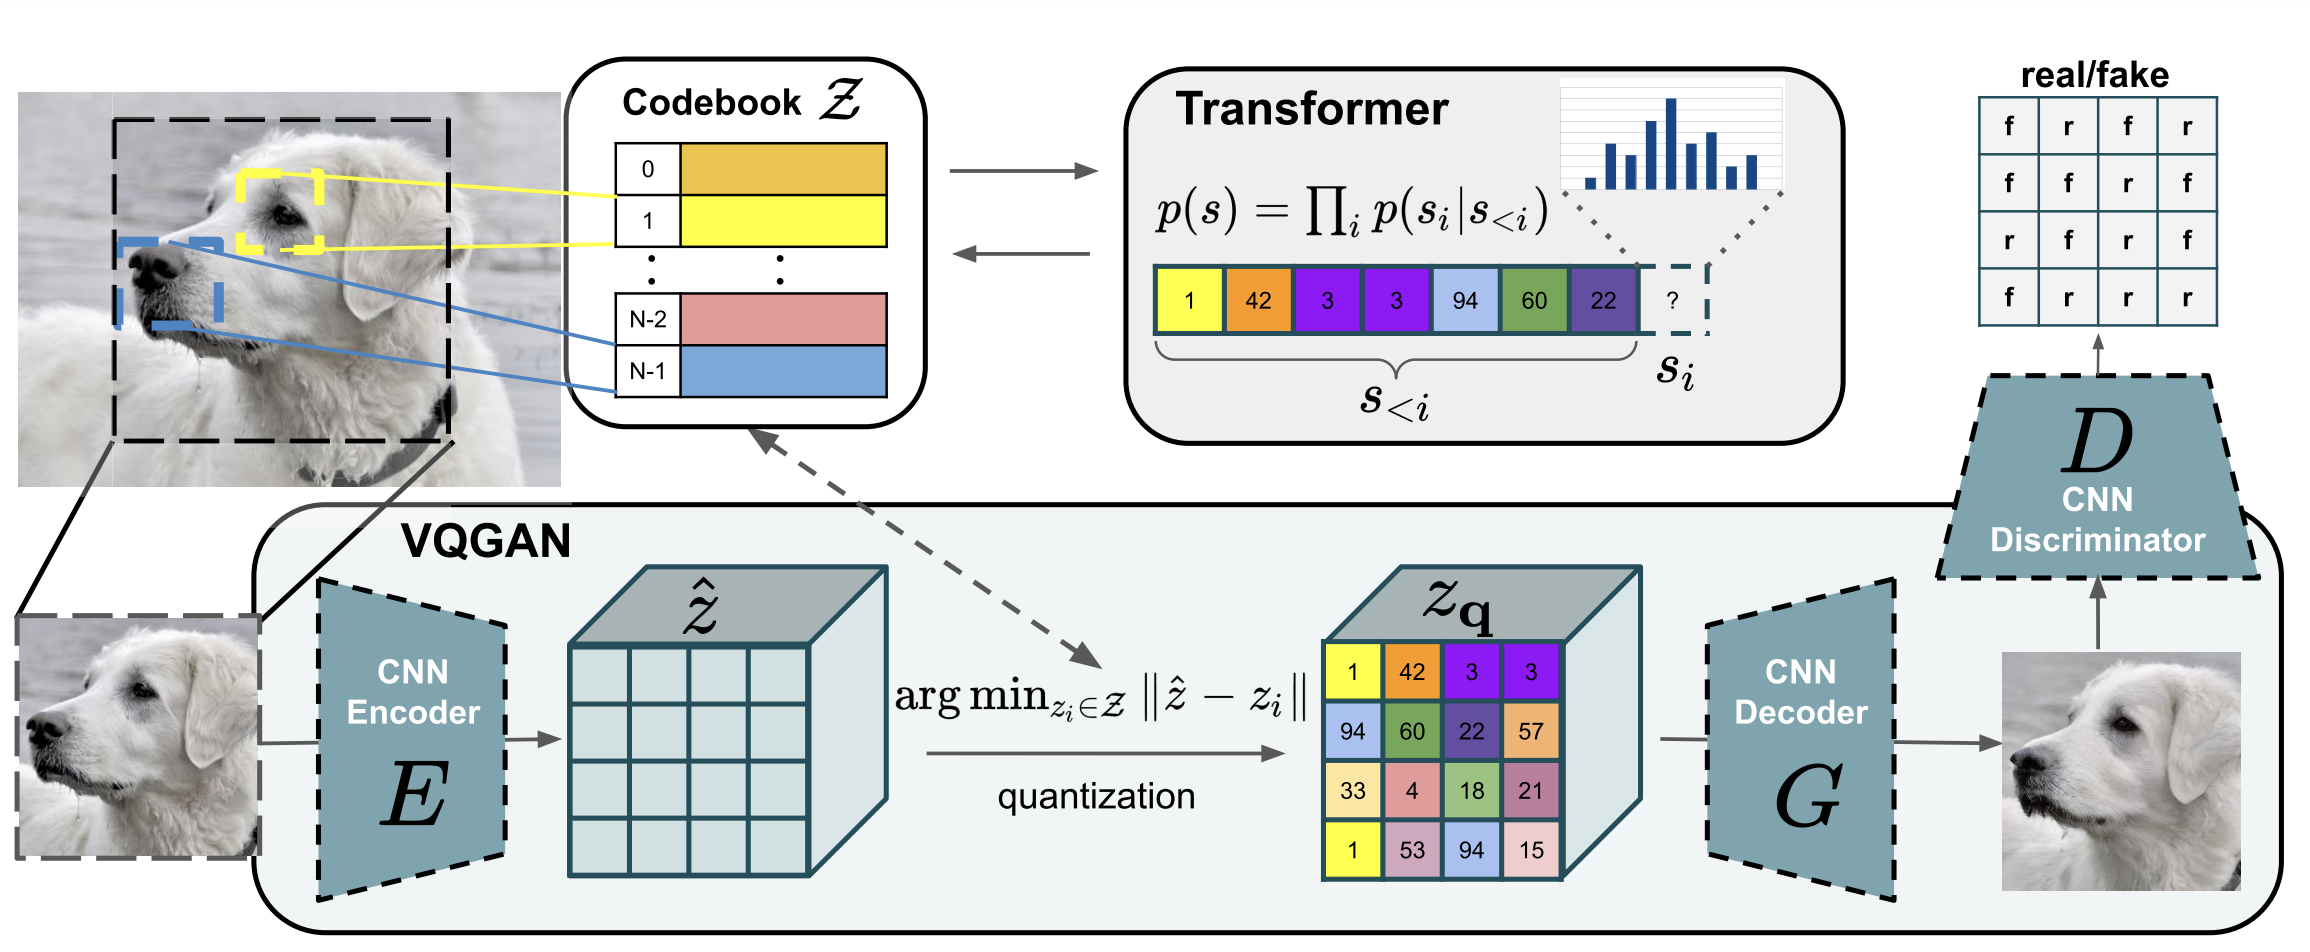
\includegraphics[width=\textwidth]{images/vqgan_architecture.png}
    \caption{VQ-GAN architecture \cite{vqgan}. The bottom rectangular part is the VQ-VAE module with the addition of a descriminator $D$ (right), and the top part is the autoregressive transformer network that predicts the next code vector $s_i$ based on previous outputs $s_{<i}$.}
    \label{fig:vqgan_architecture}
\end{figure}

In the source code of VQ-GAN the researchers used the VGG16 \cite{vgg16} architecture as the backbone of the encoder and decoder networks, but they mentioned that other architectures can be used as well, depending on the generative task. In addition, the authors used the minGPT \cite{mingpt} architecture as the transformer module (more commonly known as GPT-2, which is based on the OpenAI's model GPT-1).

The non-differential operation of quantization is a problem we saw previously in VQ-VAE (subsection \ref{subsec:vqvae_vq}), and to solve this problem the authors said that they used the straight-through estimator \cite{ste} to backpropagate the gradients through the quantization process, similarly to VQ-VAE.






\subsection{Architecture}

THe architecture of VQ-GAN is shown in figure \ref{fig:vqgan_architecture}. The training involves feeding images $x \in X$ of size $x \in \mathbb{R}^{H \times W \times 3}$ \footnote[2]{The training dataset was of size $256 \times 256 \times 3$.} to the encoder $E$ to get the latent representation $\hat{z}$ of size $\hat{z} \in \mathbb{R}^{h \times w \times n_z}$, where $n_z$ is the dimension of each codebook vector. These representation are then quantisized by the VQ module to get the discrete latent representation $z_q \in \mathbb{R}^{h \times w \times n_z}$. This operation converts latent vectors to indencies of code vectors by nearest neighbor code vector (index in the codebook points to a code vector). Using $z_q$ vectors, the CNN decoder $G$ then reconstructs the image $\hat{x}$. A discriminator $D$ is used to distinguish between real and fake (generated) pixel patches of size 16x16. This module encourages the model to generate finer details and local patterns in the image, leading to better overall quality.

The autoregressive transformer is used to predict the embeddings $z_q$ and provide the decoder $G$ the nessessary information to generate a new image, compared to PixelCNN model \cite{pixelcnn} which uses transformer for pixel-by-pixel prediction.




\subsection{Training}

The model is trained in two stages: in the first phase, the VQ module is trained to learn a discrete latent representation of the input data (learn the codebook), and the second phase trains the transformer module to predict the code vectors sequence that will be used to generate the output image.

The loss function of training the model to learn the codebook is given by: (similar to the VQ-VAE loss function in equation \ref{eq:vqvae_loss}):

\begin{equation}
    \mathcal{L}_{\text{VQ}} (E, G, \mathcal{Z}) = \Vert x - \hat{x} \Vert ^2 + \Vert \text{sg}[E(x)] - z_q \Vert ^2_2 +  \beta \Vert \text{sg}[z_q] - E(x) \Vert ^2_2
\end{equation}

where the first term is the MSE reconstruction loss (similar to equation \ref{eq:mse}), the second term is the quantization error, and the third term is the commitment loss. The reconstruction loss is intended to train the decoder $G$ to output (reconstruct latents $z_q$ to an image) images of similar distribution to the dataset. The quantization loss encourages the model to move the codebook vectors torwards the encoder outputs, so to match the encoder's output distribution (gradients are calculated for $z_q$ and not $\text{sg}[E(x)]$ because of the stop gradient operation). The commitment loss encourages the encoder to "commit" to outputting embeddings that are close to the codebook vectors.

However, instead of the MSE loss, the authors used a perceptual loss \footnote[4]{Perceptual loss measures the difference between the high-level features of two images (a generated image and an image from the dataset). Typically the high-level features are extracted by pretrained CNNs.} and \textbf{introduced an adversarial training procedure with a patch-based discriminator $D$} that tries to distinguish between real and fake pixel patches of size 16x16 of an image. The loss function of the discriminator is given by:

\begin{equation}
    \mathcal{L}_{\text{GAN}}(\{E,G,Z\}, D) = [\log D(x) + \log (1-D(\hat{x}))]
\end{equation}

If $D$ outputs 1, then the image is from the dataset (real), and if it outputs 0, then the image is fake (generated by the decoder $G$). Just like in GAN, the discreiminator objective is to maximize the probability of assigning the correct label to the input image and in the loss function the first term encourages the discriminator to output 1 because $\log D(x)$ approaches 0 when $D(x)$ approaches 1, and the second term encourages the discriminator to output 0 for fake images because $\log (1-D(\hat{x}))$ approaches 0 when $D(\hat{x})$ approaches 0.

Combining both the VQ loss and the adversarial loss, the total loss function is given by:

\begin{equation}
    \mathcal{Q^*} = \arg \min_{E, G, Z} \max_D \mathbb{E}_{x \sim p(x)} [\mathcal{L}_{\text{VQ}} + \lambda \mathcal{L}_{\text{GAN}}]
\end{equation}

The $\lambda$ hyperparameter is used to balance the contribution of adversarial loss relative to the VQ loss.

\begin{figure}
    \centering
    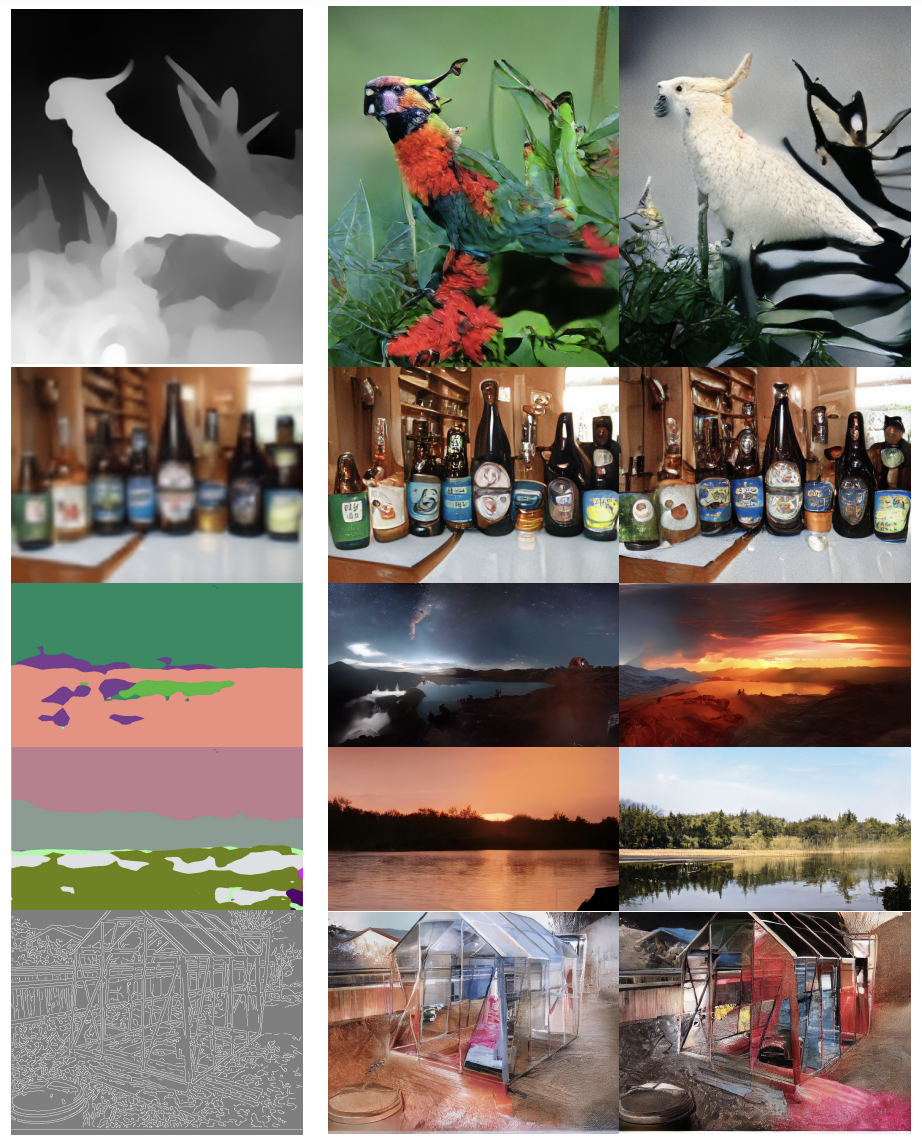
\includegraphics[width=0.5\textwidth]{images/vqgan_samples2.png}
    \caption[Caption for LOF]{Samples generated by VQ-GAN by different tasks and different resolutions. From top to bottom: depth-to-image on RIN dataset, stochastic super resolution\footnotemark on RIN dataset, 3rd and 4th row are semantic synthesis (semantic masks) on S-FLCKR dataset, and bottom row are edge synthesis on IN dataset.}
\end{figure}


\footnotetext{Super resolution is a task that generates high-resolution image from a single low-resolution image while maintaining the spatial information of the image.}

The second phase of the training involves maximizing the transformer objective. The transformer learns to predict the distribution of possible next indices, which allows us to directly maximize the log-likelihood (appendix \ref{appendix:likelihood_function}) of the data representation:

\begin{equation}
    \mathcal{L}_{\text{transformer}} = \mathbb{E}_{x \sim p(x)} [- \log p(x)]
\end{equation}

To summorize, the VQ-GAN model has 3 loss functions: the VQ loss (which trains the model to learn the codebook vectors), the adversarial loss (which trains the model to generate realistic images), and the transformer loss (which trains the model to predict the next code vector autoregressivly).







\subsection{Conditional generation}

% TODO: Finish
After the two-phase training is finished, the transformer is used to predict a sequence $s$ which is sequence of indencies to code vectors. Each token $s_i$ coresponds to an index in the codebook. So a code vector is autoregressivly predicted based on the previous tokens $s_{<i}$, which provides the nessessary embeddings $z_q$ for image synthesis ($p(s) = \prod_{i} p(s_i | s_{<i})$). If the image generation process involves a condition basis $c$, such as text, images, depth map, semantic layout or pose, then another VQ-GAN model is trained on these kind of tasks, which obtain a new codebook $Z_c$ which are the representation $r$ of $c$. Then, this representation is prepended to $s$ which restricts the computation of the negative log-likelihood to entries $p(s_i | s_{<i}, r)$. This new sequence is then given to the transformer in the first model to generate the image based on the condition $c$ (figure \ref{fig:vqgan_conditional_generation}).

\begin{figure}
    \centering
    \label{fig:vqgan_conditional_generation}
    \caption{The conditioned input sequence given to the transformer, based on the spatial condition information $c$. The middle rectangle represents a 'begin sequence' token.}
    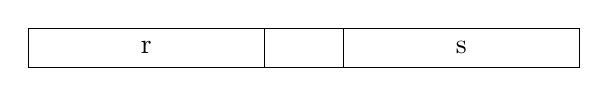
\begin{tikzpicture}
        \def \rectheight{0.5}

        % Draw the first rectangle
        \draw (0,0) rectangle (3,\rectheight);
        \node at (1.5,\rectheight / 2) {r};
        
        % Draw the middle rectangle
        \draw (3,0) rectangle (4,\rectheight);
        
        % Draw the third rectangle
        \draw (4,0) rectangle (7,\rectheight);
        \node at (5.5,\rectheight / 2) {s};
    \end{tikzpicture}
\end{figure}






\subsection{Sliding window technique for generating high-resolution images}

\begin{figure}[h]
    \centering
    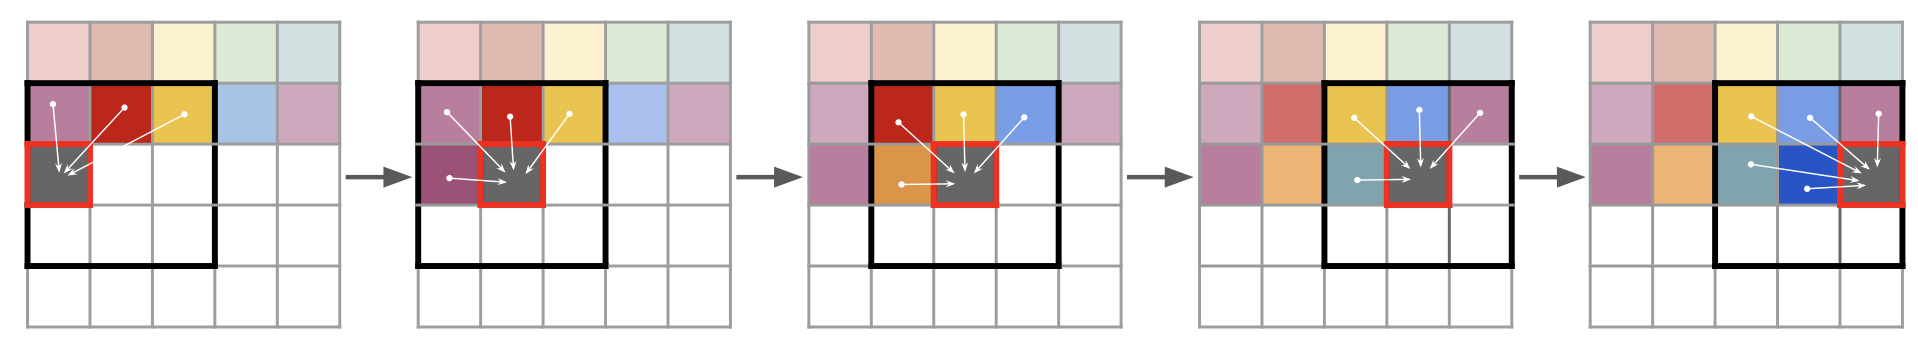
\includegraphics[width=0.75\textwidth]{images/vqgan_sliding_attention.png}
    \caption{Sliding window attention technique for generating high-resolution images. The output image is divided into patches of size 16x16=256 and by using attention mechanism, the transformer module is able to autoregressivly generate the next code vector $s_i$ based on the previous outputs $s_{<i}$ (the context).}
    \label{fig:vqgan_sliding_window}
\end{figure}

Due to the attention mechanism in transformers (quadratic computation for number of tokens, because each token requires attention to all other tokens), the model is limited in the size of the transformer sequence (in the paper they used 256 tokens). Although the encoder can reduce the dimentionality of images, the researchers noticed significant degration in generation quality. To solve this problem, they work patch-wise and crop input images to match the maximum token count in the transformer module.

To sample images, they also work patch-wise and the transformer autoregressivly predicts the next token based on the window context (figure \ref{fig:vqgan_sliding_window}).



% Diffusion models
\section{Denoise Diffusion Probabilistic Models (DDPMs)}


\subsection{Diffusion Models (DMs)}
\label{subsec:diffusion_models}

We previously talked about GANs, VAEs, and their variants (VQ-VAE, VQ-GAN). Diffusion models are also probabilistic models that define a non-linear mapping from latent variables to the observed data. Like variational autoencoders, they approximate the data likelihood using a lower bound. Diffusion models are easy to train and can produce very high-quality images compared to GANs.

A diffusion model consists of two main components: an encoder which takes a data sample $x$ and maps it through a series of intermediate latent variables $z_1, ..., z_T$, and a decoder which reverses this process, until it creates a sample image. The mappings are stochastic rather than discrete (the transformation between the latent variables involve some randomness).

In the next section, we will take a closer look at DDPMs, which is subclass of DMs. Another class of DMs is called Latent Diffusion Models (LDMs) \cite{stable_diffusion} which are based on autoencoders compressing the image space to latent space for more efficient computation.


\subsection{DDPMs}

Denoise Diffusion Probabilistic Models (DDPMs) \cite{ddpm} are a class of diffusion models that are trained to denoise images. In training phase, a dataset of images is fed to the model and DDPMs add noise to input image (it can be thought of as adding random pixel values to the input) in multiple steps (the intermediate latent variables $z_i$), unti the final result is pure noise (which will converge to the noise distribution). Then the model is trained to remove the noise and reconstruct the original image. The denoising process is called 'reverse diffusion' or reverse step and the noising process is called 'forward diffusion' or forward step. The forward diffusion step is denoted as $q(x_t | x_{t-1})$ and the reverse diffusion step is denoted as $p_\theta (x_{t-1} | x_t)$ (figure \ref{fig:ddpm_process}).

Because the addition of noise is a known stochastic process, all the learned parameters are in the decoder (the generator).

Given samples from a data distribution $q(x_0)$ we are interested in learning a model distribution $p_\theta (x_0)$ that approximates $q(x_0)$ and is easy to sample from.

DDPMs are latent variable models in the form of 

\begin{equation}
    p_\theta (x_0) = \int p_\theta(x_{0:T}) dx_{1:T} \text{,\ \ where \ \ \ } p_\theta (x_{0:T}) := p_\theta (x_T) \prod_{t=1}^{T} p_\theta (x_{t-1} | x_t)
\end{equation}

where $x_1, ..., x_T$ are latent variables. Because the integral is intractable, we use ELBO (appendix \ref{appendix:elbo}). The parameters of the model $\theta$ are learned to fit the data distribution $q(x_0)$ by maximizing a variational lower bound:

\begin{equation}
    \max_{\theta} \mathbb{E}_{q(x_0)} [\log p_\theta (x_0)] \leq \max_\theta \mathbb{E}_{q(x_0, x_1, ..., x_T)} [\log p_\theta (x_{0:T}) - \log q(x_{1:T} | x_0)]
\end{equation}

where $q(x_{1:T} | x_0)$ is some inference distribution over the latent variables. Unlike typical latent variable models (such as VAE \ref{sec:vae}), DDPMs are learned with a fixed (rather than trainable) inference procedure $q(x_{1:T} | x_0)$, and latent variables are relatively high dimensional.


\begin{figure}
    \centering
    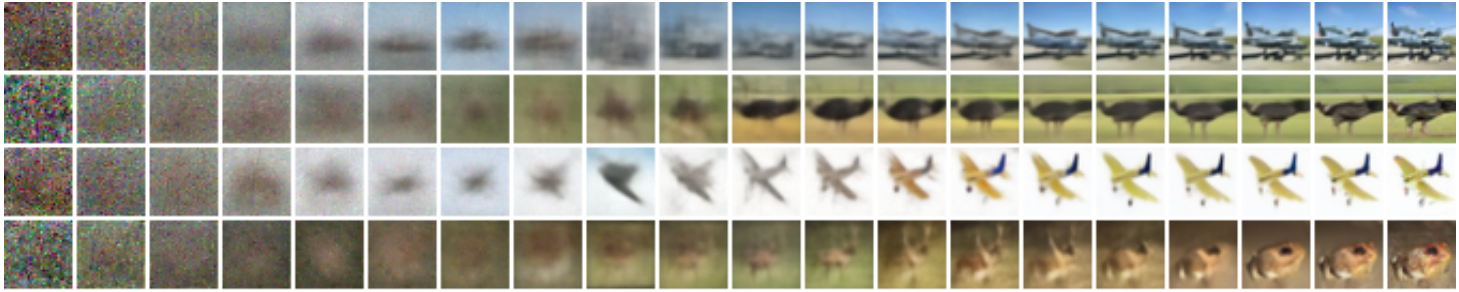
\includegraphics[width=1\textwidth]{images/diffusion_models/ddpm_denoise.png}
    \caption{Progressive generation (left to right) of unconditional CIFAR10 dataset in DDPM \cite{ddpm}.}
\end{figure}


\begin{figure}
    \centering
    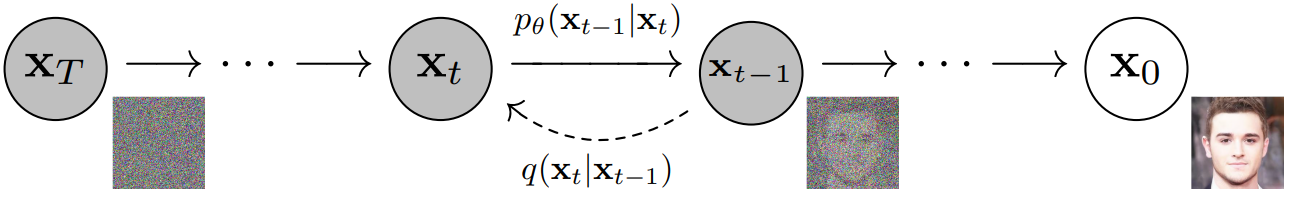
\includegraphics[width=1\textwidth]{images/diffusion_models/ddpm_process.png}
    \caption{A graph representing the forward ($q(x_t | x_{t-1})$) and reverse ($p_\theta(x_{t-1} | x_t)$) diffusion process in DDPMs \cite{ddpm}. The next step (either in forward or reverse diffusion) depends conditionally on the previous steps ($p_\theta (x_{t-1} | x_t)$ is the reverse step, and forward step is $q(x_t | x_{t-1})$).}
    \label{fig:ddpm_process}
\end{figure}






\begin{figure}[h]
    \centering
    \begin{minipage}{0.10\textwidth}  % Divide the width by 7 for 7 images
        \centering
        
\includegraphics[width=\textwidth]{images/diffusion_models/noise_to_image_gif/0.png}
    \end{minipage}
    \begin{minipage}{0.10\textwidth}
        \centering
        
\includegraphics[width=\textwidth]{images/diffusion_models/noise_to_image_gif/1.png}
    \end{minipage}
    \begin{minipage}{0.10\textwidth}
        \centering
        
\includegraphics[width=\textwidth]{images/diffusion_models/noise_to_image_gif/2.png}
    \end{minipage}
    \begin{minipage}{0.10\textwidth}
        \centering
        
\includegraphics[width=\textwidth]{images/diffusion_models/noise_to_image_gif/3.png}
    \end{minipage}
    \begin{minipage}{0.10\textwidth}
        \centering
        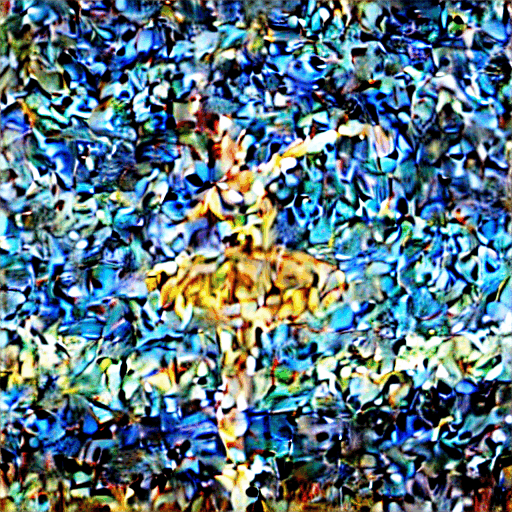
\includegraphics[width=\textwidth]{images/diffusion_models/noise_to_image_gif/4.png}
    \end{minipage}
    \begin{minipage}{0.10\textwidth}
        \centering
        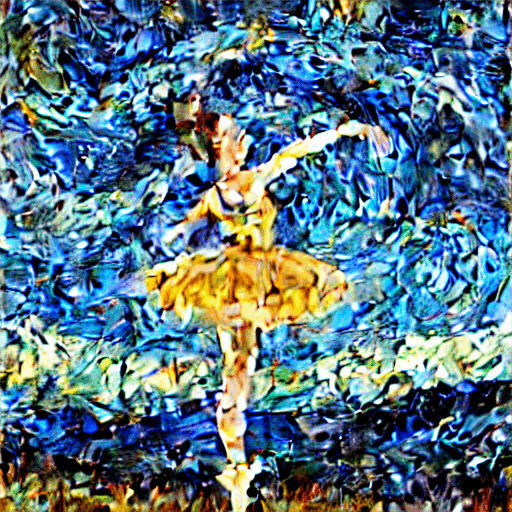
\includegraphics[width=\textwidth]{images/diffusion_models/noise_to_image_gif/5.png}
    \end{minipage}
    \begin{minipage}{0.10\textwidth}
        \centering
        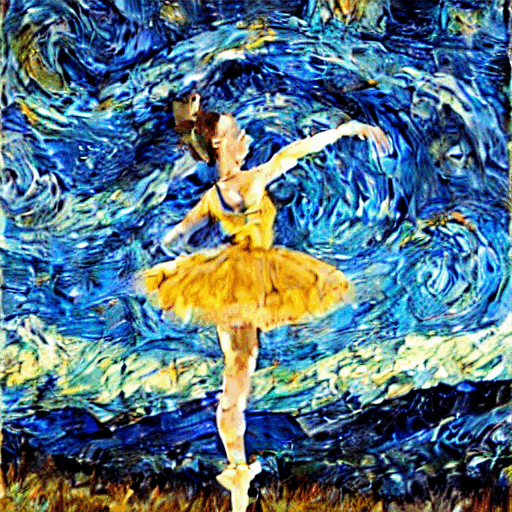
\includegraphics[width=\textwidth]{images/diffusion_models/noise_to_image_gif/6.png}
    \end{minipage}
    \begin{minipage}{0.10\textwidth}
        \centering
        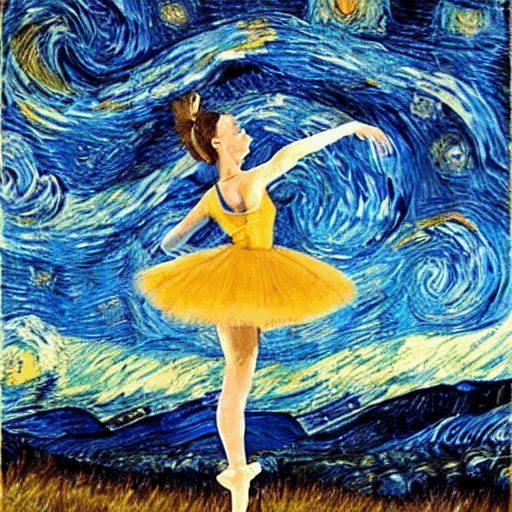
\includegraphics[width=\textwidth]{images/diffusion_models/noise_to_image_gif/7.png}
    \end{minipage}
    \caption{Progressive decoding of noise latents to an image in DDPMs \cite{ddpm}. Images taken from \href{https://scholar.harvard.edu/binxuw/classes/machine-learning-scratch/materials/stable-diffusion-scratch}{harvard university}.}
\end{figure}




\subsection{Noise Schedulers}

In the paper \cite{ddpm} the authors used linear scheduler, however OpenAI released a paper \cite{openai_improved_ddpm} that uses cosine scheduler. They have shown that a cosine scheduler performs better than a linear scheduler in terms of image generation quality (see figure \ref{fig:linear_cosine_scheduler}).

\begin{figure}
    \centering
    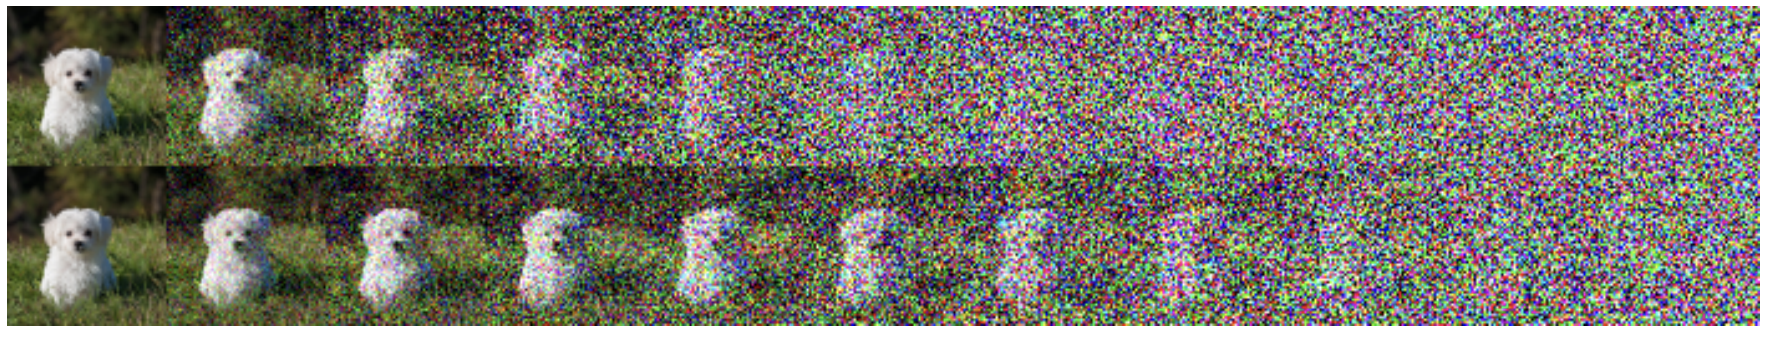
\includegraphics[width=1\textwidth]{images/diffusion_models/linear_cosine_scheduler.png}
    \caption{Linear scheduler (top, \cite{ddpm}) and cosine scheduler (bottom, \cite{openai_improved_ddpm}) shows that linear scheduler adds noise too quickly which degrades the model's performance whereas cosine scheduler adds noise more slowly.}
    \label{fig:linear_cosine_scheduler}
\end{figure}







\subsection{Encoder}

The forward diffusion process maps a data image $x$ through a series of intermediate variables $z_1, ..., z_T$ with the dimension as $x$ according to the following recursion:

\begin{equation}
    \begin{aligned}
    \mathbf{z}_1 &= \sqrt{1 - \beta_1} \cdot \mathbf{x} + \sqrt{\beta_1} \cdot \epsilon_1, \\
    &\;\;\vdots \notag \\
    \mathbf{z}_t &= \sqrt{1 - \beta_t} \cdot \mathbf{z}_{t-1} + \sqrt{\beta_t} \cdot \epsilon_t \quad \forall \, t \in \{2, \ldots, T\}
    \end{aligned}
\end{equation}

At each step $i \in {1, 2, ..., t, t+1, ..., T}$ a noise vector $e_i$ is drawn from a standard normal distribution. This equation adds random noise $e_i$ to the data (image) $x = z_0$ and $\beta$ is a schedule function ($\beta(t):[1, ..., T] \rightarrow \mathbb{R}$) that determines the amount of noise added at each step ($\beta$ is a variance schedule, which can be linear, cosine, quadratic and more). 

A more formal notation for the forward process is:

\begin{equation*}
    \begin{aligned}
        q(x_t | x_{t-1}) = \mathcal{N}(x_t; \sqrt{1-\beta_t} \cdot x_{t-1}, \beta_t \mathbf{I}) \\
        q(x_{1:T} | x_0) = \prod_{t=1}^{T} q(x_t | x_{t-1})
    \end{aligned}
\end{equation*}

In the above formula we can see that to define the next timestep $x_t$ and to get a noisier image, we define it as gaussian / normal distribution where the mean is $\sqrt{1-\beta_t} x_{t-1}$ and variance $\beta_t \mathbf{I}$. The $\beta$ parameter is the noise scheduler (how much noise we add at each step). This process is known as Markov Chain, since the next step depends only on the previous step (see appendix \ref{appendix:markov_chains}).

An interesting point the authors made is that its possible to sample $x_t$ from any arbitrary timestep $t$, given the original image $x_0$ (without calculating all the intermediate steps):

\begin{equation}
    \begin{aligned}
    q(\mathbf{x}_t|\mathbf{x}_0) = \mathcal{N}(\mathbf{x}_t; \sqrt{\bar{\alpha}_t}\mathbf{x}_0, (1 - \bar{\alpha}_t)\mathbf{I}) \\
    \text{where } \alpha_t := 1 - \beta_t \text{ and } \bar{\alpha}_t := \prod_{i=1}^{t} \alpha_i
    \end{aligned}
    \label{eq:forward_diffusion}
\end{equation}

Equation \ref{eq:forward_diffusion} describes the process of adding noise, $x_t$ from $x_0$ without any intermediate steps.

Since $\alpha$ depends on $\beta$ and $\beta$ is a noise scheduler (fixed), there are no parameters to learn in the forward process.

Each diffusion model has slightly different implementation in its network, and this encoder formulation generalizes the encoder process. We will take a closer look on the encoder/decoder network in the Stable Diffusion paper \cite{stable_diffusion} in the next section \ref{sec:stable_diffusion} and its code implementation.










\subsection{Decoder}

The decoder removes noise from the intermediate latent variables $z_1, ..., z_T$ and reconstructs the original image $x$ using the following recursion:

\begin{equation}
    p_\theta(\mathbf{x}_{t-1} | \mathbf{x}_t) = \mathcal{N}(\mathbf{x}_{t-1}; \mu_\theta(\mathbf{x}_t, t), \Sigma_\theta(\mathbf{x}_t, t))
    \label{eq:reverse_diffusion}
\end{equation}

where $\theta$ are the learned parameters of the model. The mean $\mu_\theta$ and variance $\Sigma_\theta$ are unknown and should be learned in the training stage. However, in the DDPM paper \cite{ddpm} the auhtors said:

\begin{quote}
    \textit{"We also see that learning reverse process variances (by incorporating a parameterized diagonal $\Sigma_\theta(x_t)$ into the variational bound) leads to unstable training and poorer sample quality compared to fixed variances."} \cite{ddpm}
\end{quote}

The OpenAI team released a paper titled "Improved denoising diffusion probabilistic models" \cite{openai_improved_ddpm} in which the authors used cosine noise (instead of linear in the original paper \cite{ddpm}) scheduler and also learned the variance, which significantly improved the model's performance.








\subsection{Loss function}

The loss function of DDPMs is typically the ELBO loss function (negative log-likelihood \ref{eq:elbo}):

\begin{equation*}
    \mathbb{E}[-\log p_\theta (x_0)] \leq \mathbb{E}_q[-\log \frac{p_\theta(x_{0:T})}{q(x_{1:T}|x_0)}] = \mathcal{L}
\end{equation*}

The left term is the negative log likielihood. The upper bound is the tractable ELBO loss function. The dominator $q(x_{1:T}|x_0)$ is the forward diffusion process (adds noise) and the numerator $p_\theta(x_{0:T})$ is the model's joint distribution over latent steps $x_1, ..., x_T$ which is the reverse process. The ratio of these two terms is the ELBO loss function, when this ratio reaches 1 it indicates that the model can undo the forward process. We also don't write $q_\theta$ because the forward process is not learned, only the reverse process is leanred.

Like we discussed before, diffusion models are latent variable models in the form of $p_\theta (x_0) := \int p_\theta(x_{0:T}) d\mathbf{x}_{1:T}$ which is intractable. Which is why we use the ELBO loss function to approximate the likelihood of the data (see appendix \ref{appendix:elbo}).






\subsection{Training}

The training of diffusion models is done by sampling a batch of images from the dataset, and then adding noise to the images in the forward diffusion process. The model is trained to remove the noise and reconstruct the original image in the reverse diffusion process. The loss function is the ELBO loss function (see previous section). Usually, the model is trained using stochastic gradient descent (SGD), but more advanced optimizers like Adam can be used as well.

\begin{figure}
    \centering
    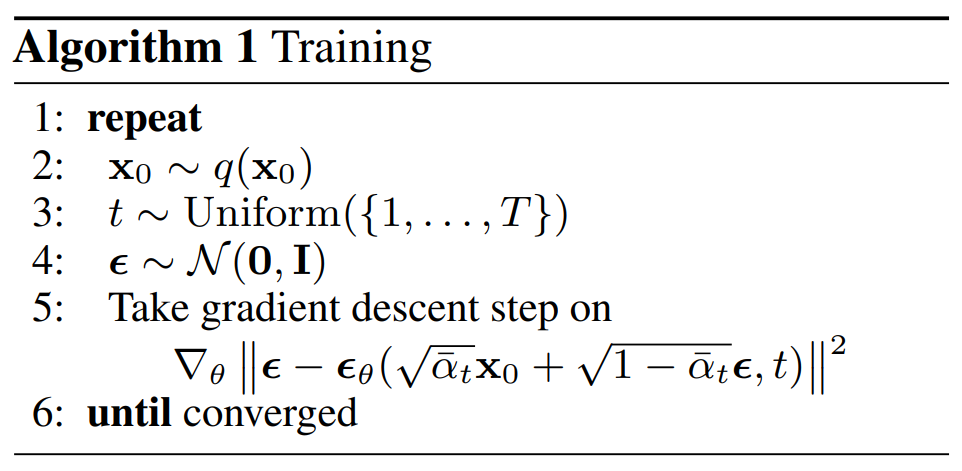
\includegraphics[width=0.5\textwidth]{images/diffusion_models/training.png}
    \caption{The training algorithm of diffusion models \cite{ddpm}. Line 2: we take a sample from the dataset. Line 3: we generate random number between 1 and T uniformly. Line 4: we sample some noise. Line 5: we calculate the gradients of the loss function.}
    \label{fig:ddpm_training}
\end{figure}

In figure \ref{fig:ddpm_training} line 5, we try to optimize the model's parameters $\theta$ by gradient decent. $\epsilon_\theta$ is the predicted noise added at timestep $t$ (a function approximator with 2 parameters that intends to predict $\epsilon$ from $x_t$) where the first parameter is the noisy image at timestep $t$, and the second parameter is the timestep ($t$). 








\section{Stable Diffusion}
\label{sec:stable_diffusion}


\begin{figure}
    \centering
    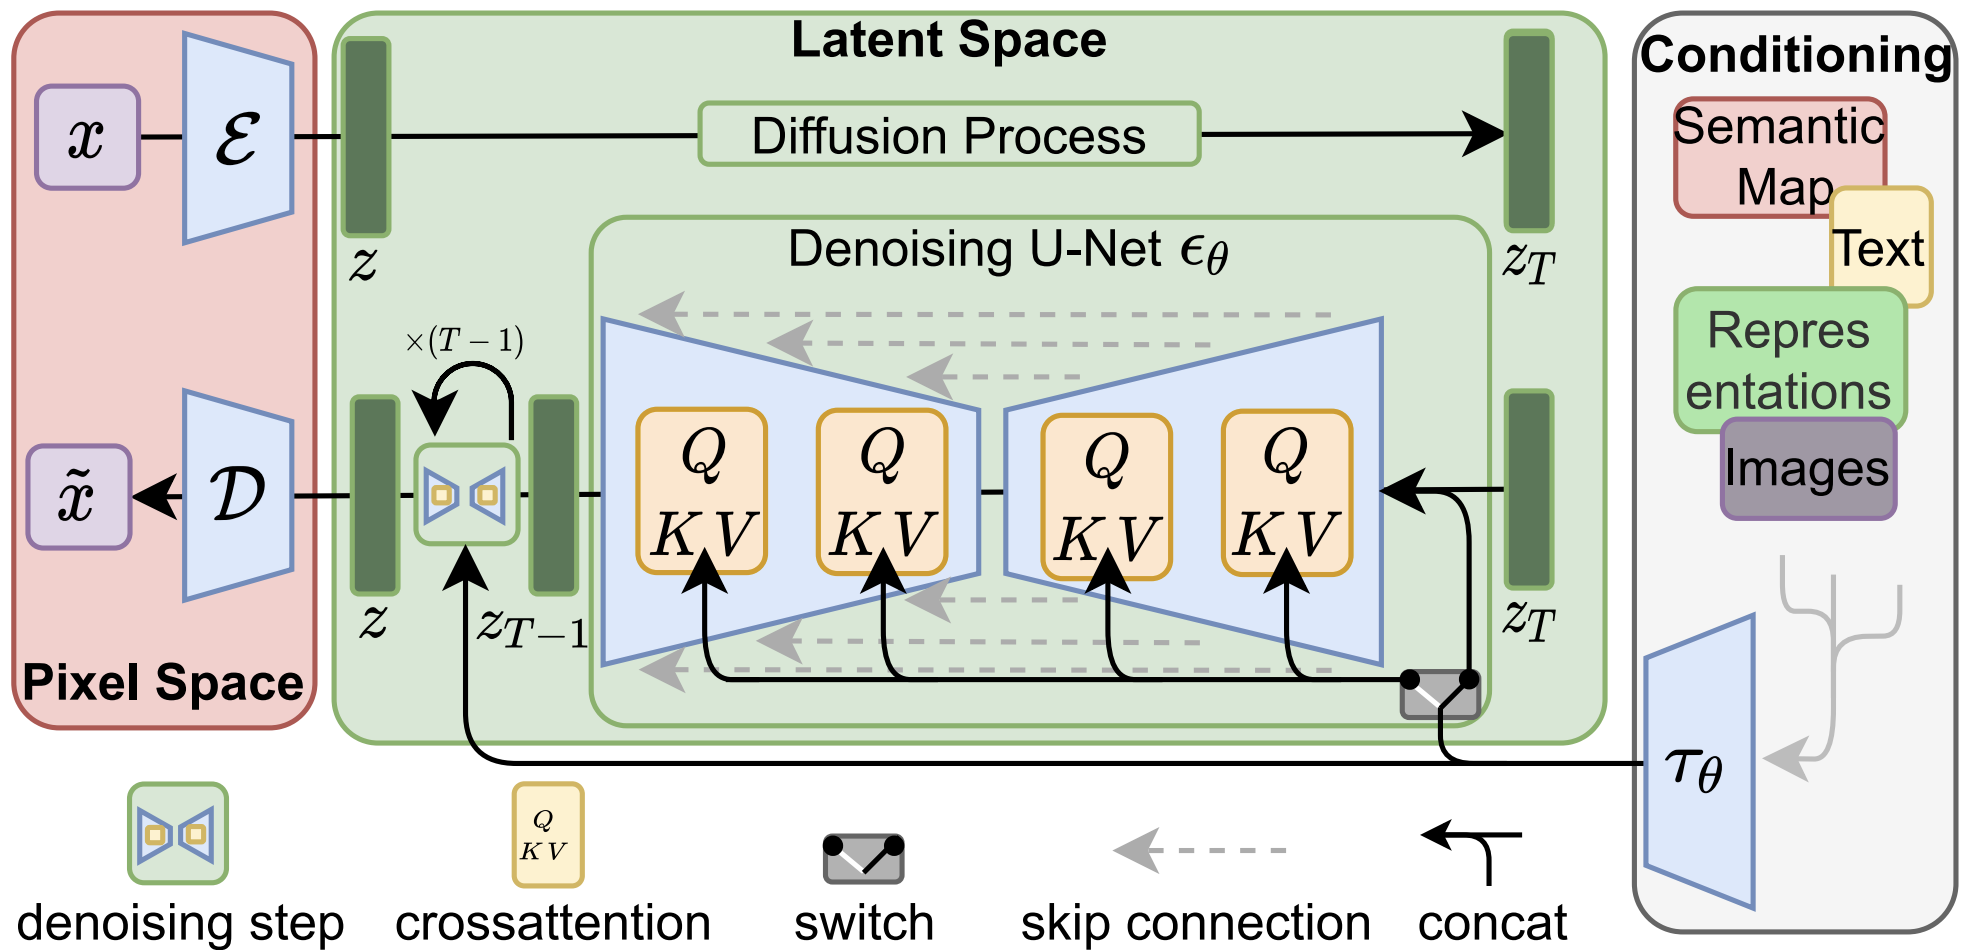
\includegraphics[width=0.6\textwidth]{images/diffusion_models/stable_diffusion/stable_diffusion.png}
    \caption{Stable diffusion scales better compared to other models \cite{stable_diffusion} (DALL-E, VQ-GAN) with less downsampling blocks ($f = 4$ instead of 16 as needed by VQ-GAN).}
\end{figure}


In the Stable Diffusion paper \cite{stable_diffusion} the authors suggested that computing gradients directly in DDPMs on the pixel space is inefficient, since this space is highly-dimensional and includes undesired high-frequency details. They suggest to convert the input images to a lower-dimensional latent representations and then apply the diffusion processes. The authors showed that this approach \textbf{scales better} and is more compute efficient \footnote{In the Stable Diffusion paper \cite{stable_diffusion} the authors showed that the model can be trained on a single GPU with 16GB of memory on images of $256\times 256$ resolution using CelebA-HQ dataset with 30 diffusion steps.} compared to working in pixel space. Moreover, the authors introduced general purpose \textbf{conditioning mechanism based on cross-attention} which allows multi-modal training.

A 2021 paper released by OpenAI \cite{openai_diffusion_beats_gans} shows that \textbf{diffusion models can outperform GANs} in terms of image fidelity by trading off diversity.











\subsection{The U-Net backbone}
\label{subsec:stable_diffusion_u_net_backbone}

U-Net (first introduced in 2015) \cite{unet} is a convolutional neural network (CNN) architecture that is commonly used in diffusion models. U-Net is used as a backbone for denoising the latent variables $z_1, ..., z_T$. The U-Net architecture is a symmetric encoder-decoder network with skip connections between the encoder and decoder: the skip connections help the network to learn better by minimizing the \textbf{exploding / vanishing gradient problems} \cite{exploding_vanishing_gradients}.

\begin{figure}
    \centering
    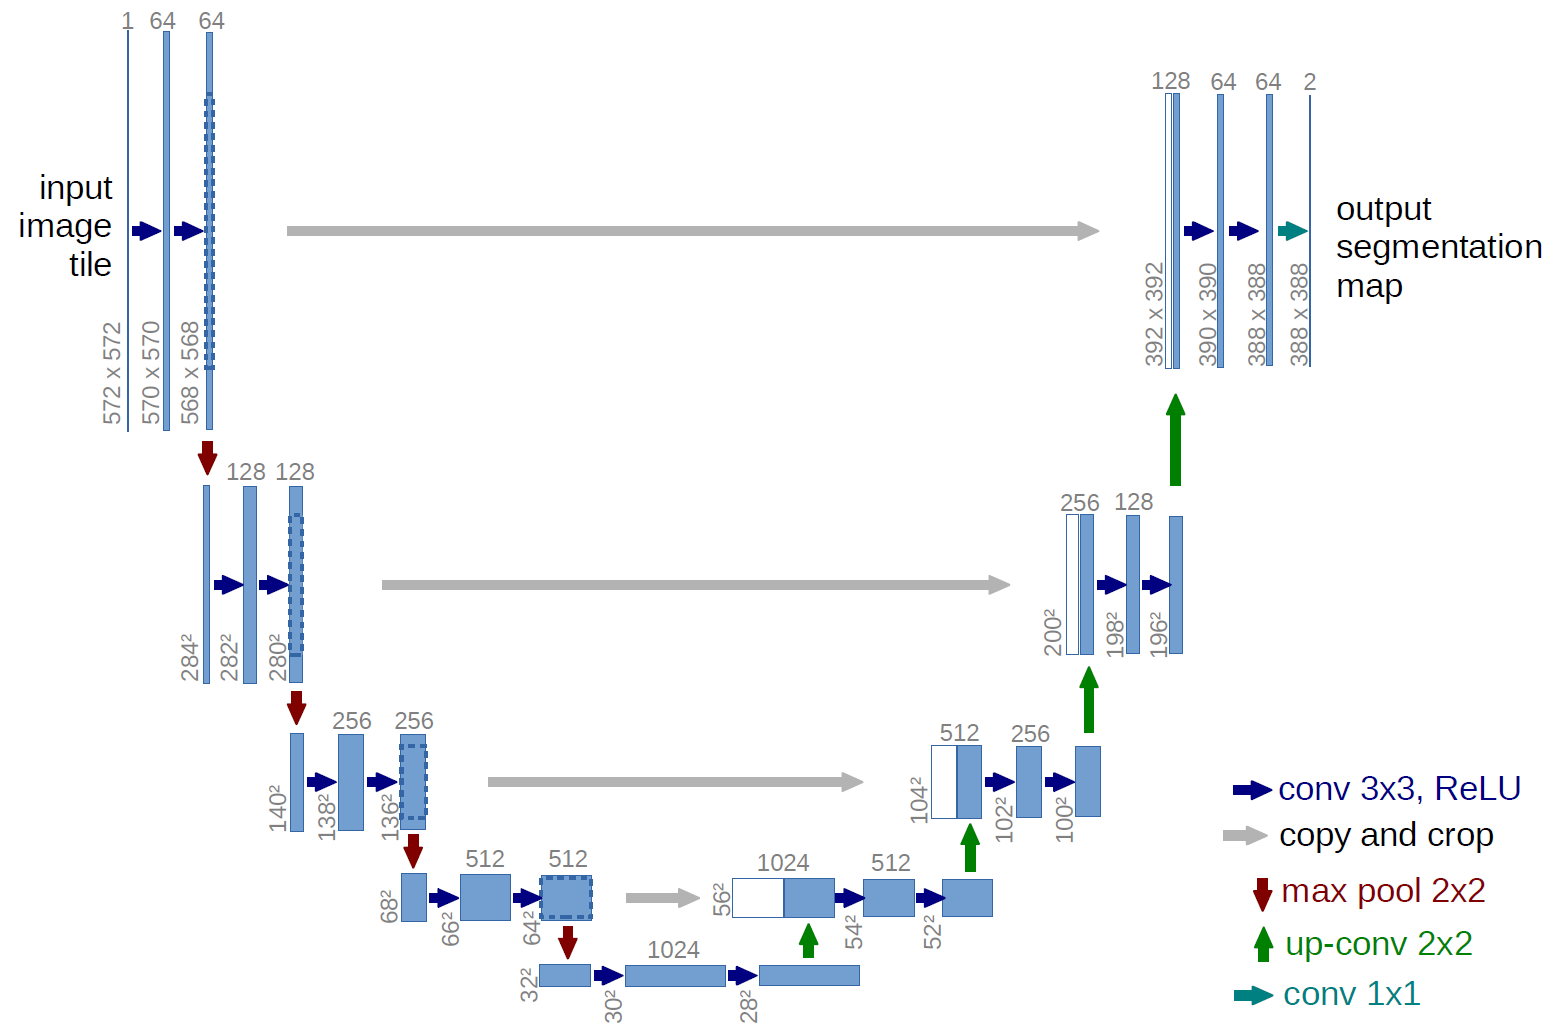
\includegraphics[width=0.5\textwidth]{images/diffusion_models/stable_diffusion/u-net-architecture.png}
    \caption{The U-Net architecture \cite{unet} with convolutional and deconvolutional layers \& skip connections.}
    \label{fig:unet_architecture}
\end{figure}

In figure \ref{fig:unet_architecture} the U-Net is shaped like a 'U' in which the input is downsampled to low spatial resolution and high feature channels and then upsampled back again. The convolution kernel size is 3x3 and they use ReLU activation function.








\subsection{Sinusoidal embeddings}
\label{subsec:sinusoidal_embeddings}

The diffusion process uses \textbf{timestep embeddings} which is a scalar representing the current diffusion timestep: $t \in [0, T]$. This way the model knows if its in the beginning of the diffusion or at the late stage, which is essential for removing noise. 

To get the embeddings, the timestep is first projected into a \textbf{sinusoidal embedding}, similar to the way positional encodings are used in transformers.

\begin{figure}[h]
    \centering
    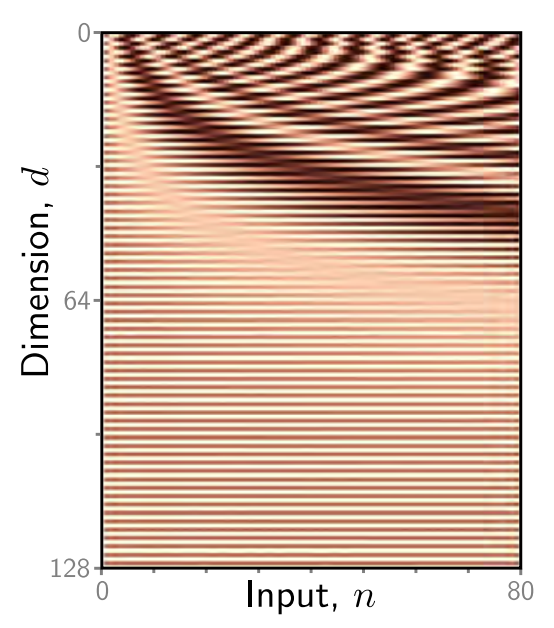
\includegraphics[width=0.25\textwidth]{images/diffusion_models/stable_diffusion/positional_encodings.png}
    \caption{Sinusoidal positional embeddings used in a transformers \cite{understanding_deep_learning_book_2024}. \textit{X axis}: the input scalar (position in a transformer or timestep in diffusion model). \textit{Y axis}: the embeddings dimensions \cite{understanding_deep_learning_book_2024}.}
    \label{fig:sinusoidal_embeddings}
\end{figure}

In figure \ref{fig:sinusoidal_embeddings} we can see the sinusoidal positional embeddings used in a transformer model, which is similar to timestep embeddings. The pattern is sinusoidal where lighter regions indicate lower values and darker regions indicate higher values. Each column in the X axis is a \textbf{unique embedding}. For example, the scalar '1' will have different encodings than a scalar '2', which helps distinguish the position / timestep of the input sequence.

\begin{lstlisting}[language=Python, breaklines=true, caption={Timestep embeddings in Stable Diffusion: we convert the timestep to an embedding.}, label={lst:timestep_embeddings_stable_diffusion}]
def get_time_embedding(timestep):
    # Shape: (160,)
    freqs = torch.pow(10000, -torch.arange(start=0, end=160, dtype=torch.float32) / 160) 
    # Shape: (1, 160)
    x = torch.tensor([timestep], dtype=torch.float32)[:, None] * freqs[None]
    # Shape: (1, 160 * 2)
    return torch.cat([torch.cos(x), torch.sin(x)], dim=-1)
\end{lstlisting}

The general formula for timestep embeddings is given in equation \ref{eq:timestep_embeddings}. The code snippet in listing \ref{lst:timestep_embeddings_stable_diffusion} is taken from \href{https://github.com/hkproj/pytorch-stable-diffusion/blob/e0cb06de011787cdf13eed7b4287ad8410491149/sd/pipeline.py#L164}{a re-implementation of Stable Diffusion}.

\begin{equation}
    \text{Enc}_i(t) =
    \begin{cases}
        \sin\left(\frac{t}{10000^{\frac{2i}{d}}}\right) & \text{if } i \text{ is even} \\
        \cos\left(\frac{t}{10000^{\frac{2i}{d}}}\right) & \text{if } i \text{ is odd}
    \end{cases}
    \label{eq:timestep_embeddings}
\end{equation}










\subsection{Architecture}

\begin{figure}
    \centering
    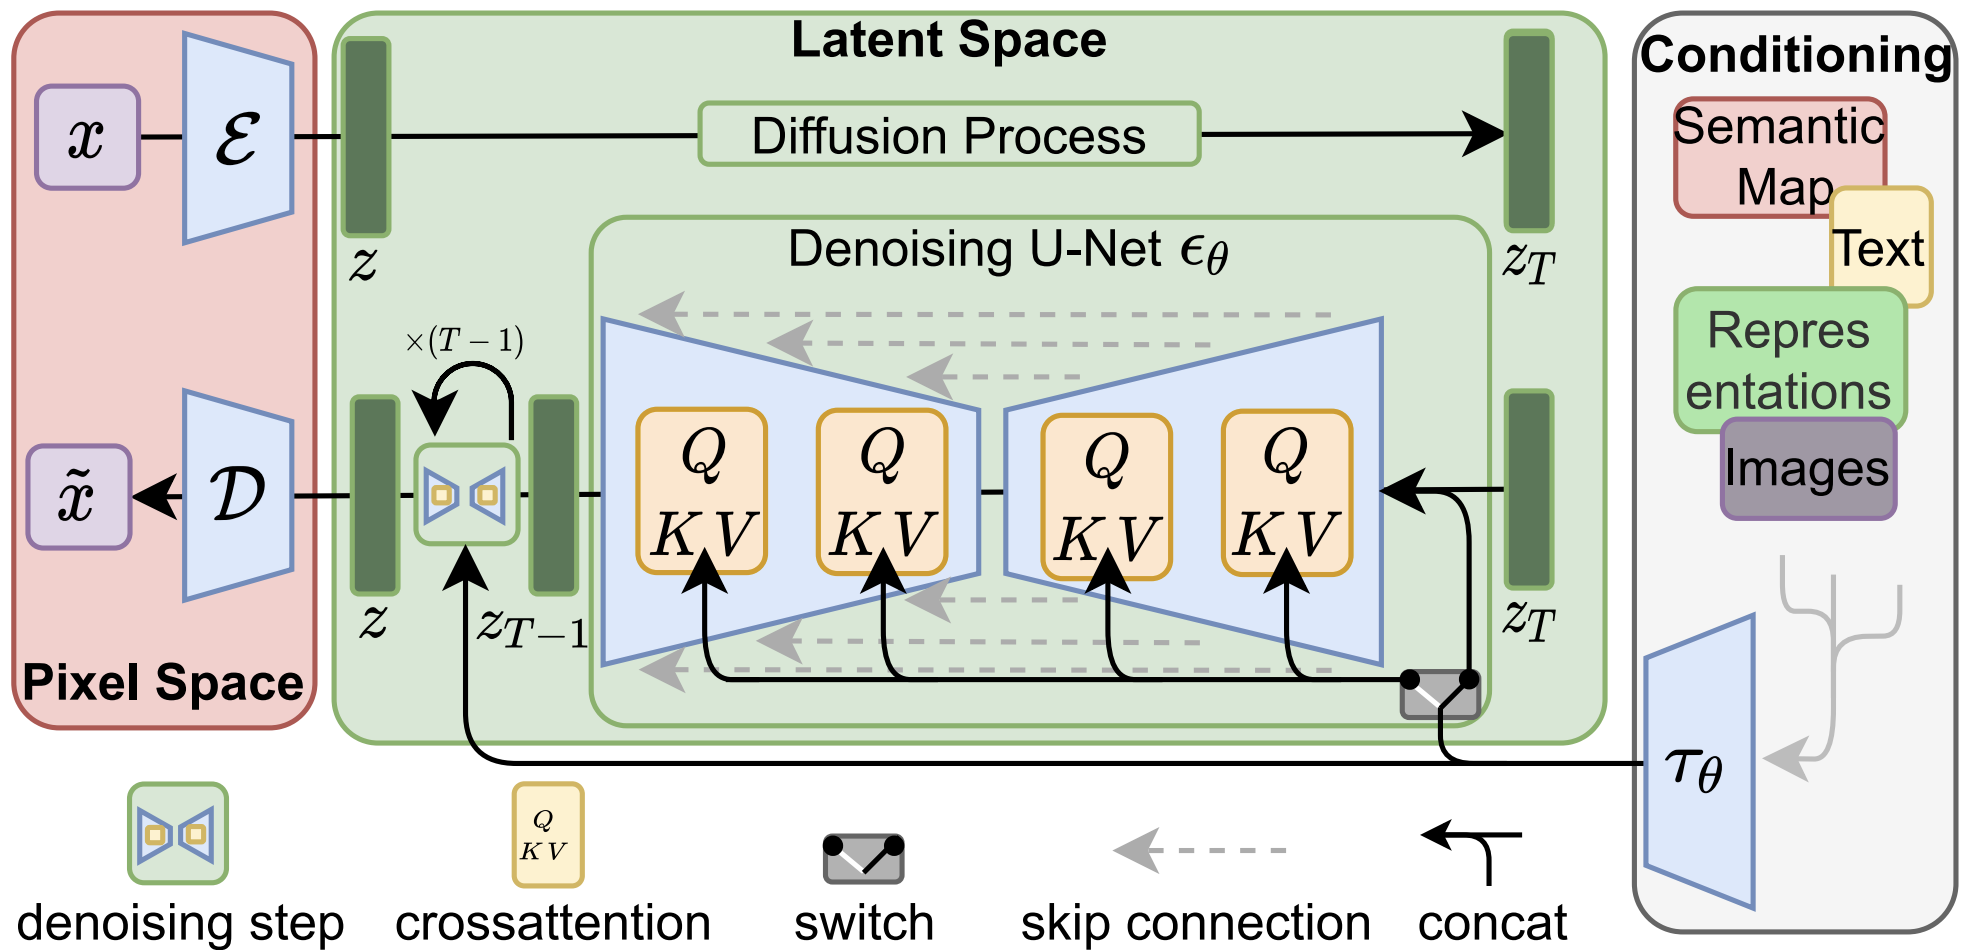
\includegraphics[width=0.5\textwidth]{images/diffusion_models/stable_diffusion/architecture.png}
    \caption{Stable Diffusion architecture \cite{stable_diffusion}.}
    \label{fig:stable_diffusion_architecture}
\end{figure}

The high-level architecture is shown in figure \ref{fig:stable_diffusion_architecture}. The stable diffusion model, which is a latent diffusion model (LDM), consists of: 

\begin{itemize}
    \item Variational autoencoder (VAE) which compresses the input images into regularized latent space. It consists of:
    \begin{itemize}
        \item Encoder $\varepsilon$ which converts the input images $x$ to latent space $z$.
        \item Decoder $\mathcal{D}$ which converts the latent vector $z$ back to the pixel space $\tilde{x}$.
    \end{itemize}
    \item A U-Net backbone which which serves as the noise prediction network, predicts the noise needed to denoise the intermediate latent vectors $z_T, ..., z_1$ in each step. It incorporates timestep embeddings as an essential input.
    \item A domain specific encoder $\tau_\theta$ which encodes the conditional information (text prompts, images, segmentation masks) into tokens which will be used in the cross-attention layers, or concatenated with the latent vector (the switch mechanism).
\end{itemize}







\subsection{Conditioning}

Cross-attention (appendix \ref{appendix:attention}) is used in Stable Diffusion for \textbf{multi-modal conditioning}: it guides the model to output images based on conditional information. Although this information is multi-modal (e.g. images, text, segmentation masks), the cross-attention layers in the U-Net and the switch mechanism able to process them all.

\textbf{Text conditioning}: if the conditioning signal is text prompt, the domain specific encoder $\tau_\theta$ is a text encoder (tokenizer) which converts the text words to embeddings (tokens). In the paper \cite{stable_diffusion} the authors used a \href{https://github.com/CompVis/latent-diffusion/blob/a506df5756472e2ebaf9078affdde2c4f1502cd4/ldm/modules/encoders/modules.py#L138}{\textbf{frozen CLIPTokenizer}}, which is a pre-trained tokenizer trained on specific vocabulary, and special tokens (beginning of sentence, end of sentence, padding, mask tokens and more). However, digging into the source code, you will find other text encoders as well such as \href{https://github.com/CompVis/latent-diffusion/blame/a506df5756472e2ebaf9078affdde2c4f1502cd4/ldm/modules/encoders/modules.py#L53}{\textbf{BERT}} \cite{bert}.

\textbf{Switch mechanism}: In figure \ref{fig:stable_diffusion_architecture} the 'switch' in the diagram is used for different kinds of conditional information. If the conditional information is spatial (such as images, layouts, semantic masks), they use concatenation with $z_T$. In the case of text (not spatial), they use cross-attention layers. 

We dive deeper into self-attention, multi-head attention and cross-attention in the appendix \ref{appendix:attention}, which are commonly used in other image and video synthesis models.













\subsection{Classifier-free diffusion guidance (CFG)}

\label{subsec:classifier_free_diffusion_guidance}

Classifier-free guidance (CFG) (see section \ref{subsec:classifier_free_diffusion_guidance}) is used in Stable Diffusion to control the influence of the conditioning signal and balance between being faithful to the conditioning signal or being diverse in the generated samples.

So far we have focused on modeling just the data distribution $p(x)$. However, we are often also interested in learning conditional distribution $p(x|y)$, which would enable us to explicitly control the data we generate through conditioning signal $y$.

We can add conditioning information alongside the timestep information, at each iteration:

\[
p(x_{0:T}) = p(x_T) \prod_{t=1}^{T} p_\theta (x_{t-1} | x_{t, y})
\]

When training a diffusion model to generate images based on specific conditional information, there's a risk that the model might not fully consider or even ignore these conditions, using this vanilla formulation. To address this, a technique called "guidance" is used. Guidance allows us to explicitly control \textbf{how much influence the conditions have on the generated images}, but this can sometimes lead to less variety in the results. In other words, we use weight to control how much the model should pay attention to the conditioning signal.


Conditioning a generative model can be achieved through two methods: 

\begin{itemize}
    \item classifier guidance
    \item and classifier-free guidance.
\end{itemize}





\subsubsection*{Classifier guidance}

Classifier guidance \cite{openai_diffusion_beats_gans} involves \textbf{training a separate model} to condition the output, and is based on score-based diffusion models \cite{score_based_generative_modeling}. 

Classifier guidance formulation is given as:

\[
\nabla \log p(x_t | y) = \underbrace{\nabla \log p(x_t)}_{\text{unconditional score}} + \underbrace{\gamma \nabla \log p(y | x_t)}_{\text{adversarial gradient}}
\]

where $\gamma$ is a hyperparameter that controls the strength of the conditioning signal in classifier guidance method.








\subsubsection*{Classifier-free guidance}

In Classifier-free guidance (CFG) \cite{classifier_free_guidance}, instead of training two networks, one conditional network and an unconditional network, we train a single network, and during training, \textbf{we set the conditioning signal to zero} with some probability. This way, the network becomes a mix of conditioned and unconditioned networks, and we can take the conditioned and unconditioned output and combine them with weight that indicates how much we want the network to pay attention to the conditioning signal. 

The formulation for classifier-free guidance is given by:

\[
\nabla \log p(x_t | y) = \underbrace{\gamma \nabla \log p(x_t | y)}_{\text{conditional score}} + \underbrace{(1 - \gamma) \nabla \log p(x_t)}_{\text{unconditional score}}
\]

In contrast to classifier guidance, classifier-free guidance streamlines the training process and lowers computational costs by utilizing a single model instead of training two separate models.

\begin{lstlisting}[language=Python, caption={Classifier-free guidance (CFG) in Stable Diffusion.}, label={lst:cfg_stable_diffusion}]
if do_cfg:
    output_cond, output_uncond = model_output.chunk(2)
    model_output = cfg_scale * (output_cond - output_uncond) + output_uncond
\end{lstlisting}

In listing \ref{lst:cfg_stable_diffusion} the code snippet is taken from \href{https://github.com/hkproj/pytorch-stable-diffusion/blob/e0cb06de011787cdf13eed7b4287ad8410491149/sd/pipeline.py#L135C1-L136C1}{a re-implementation of Stable Diffusion}, but the official implementation of Stable Diffusion is \href{https://github.com/CompVis/stable-diffusion/blob/21f890f9da3cfbeaba8e2ac3c425ee9e998d5229/ldm/models/diffusion/ddim.py#L178C1-L179C1}{very similar}.

















\subsection{Contrastive Language Image Pre-training (CLIP)}
\label{subsec:clip}

In Stable Diffusion, the authors used CLIP as the text encoder for the conditional text prompts.

CLIP (Contrastive Language Image Pre-training) \cite{openai_clip} is a model developed by OpenAI that learns visual concepts from text supervision. The model builds \textbf{associations between images and text prompts}. Often this association is called 'text-image alignment', or 'image-text alignment'. It models how well a generated image corresponds to its associated text description.

The \textbf{CLIPTokenizer}, which is part of the CLIP model, converts text prompts to a sequence of tokens which are then used in the latent space of the Stable Diffusion model.

\begin{figure}
    \centering
    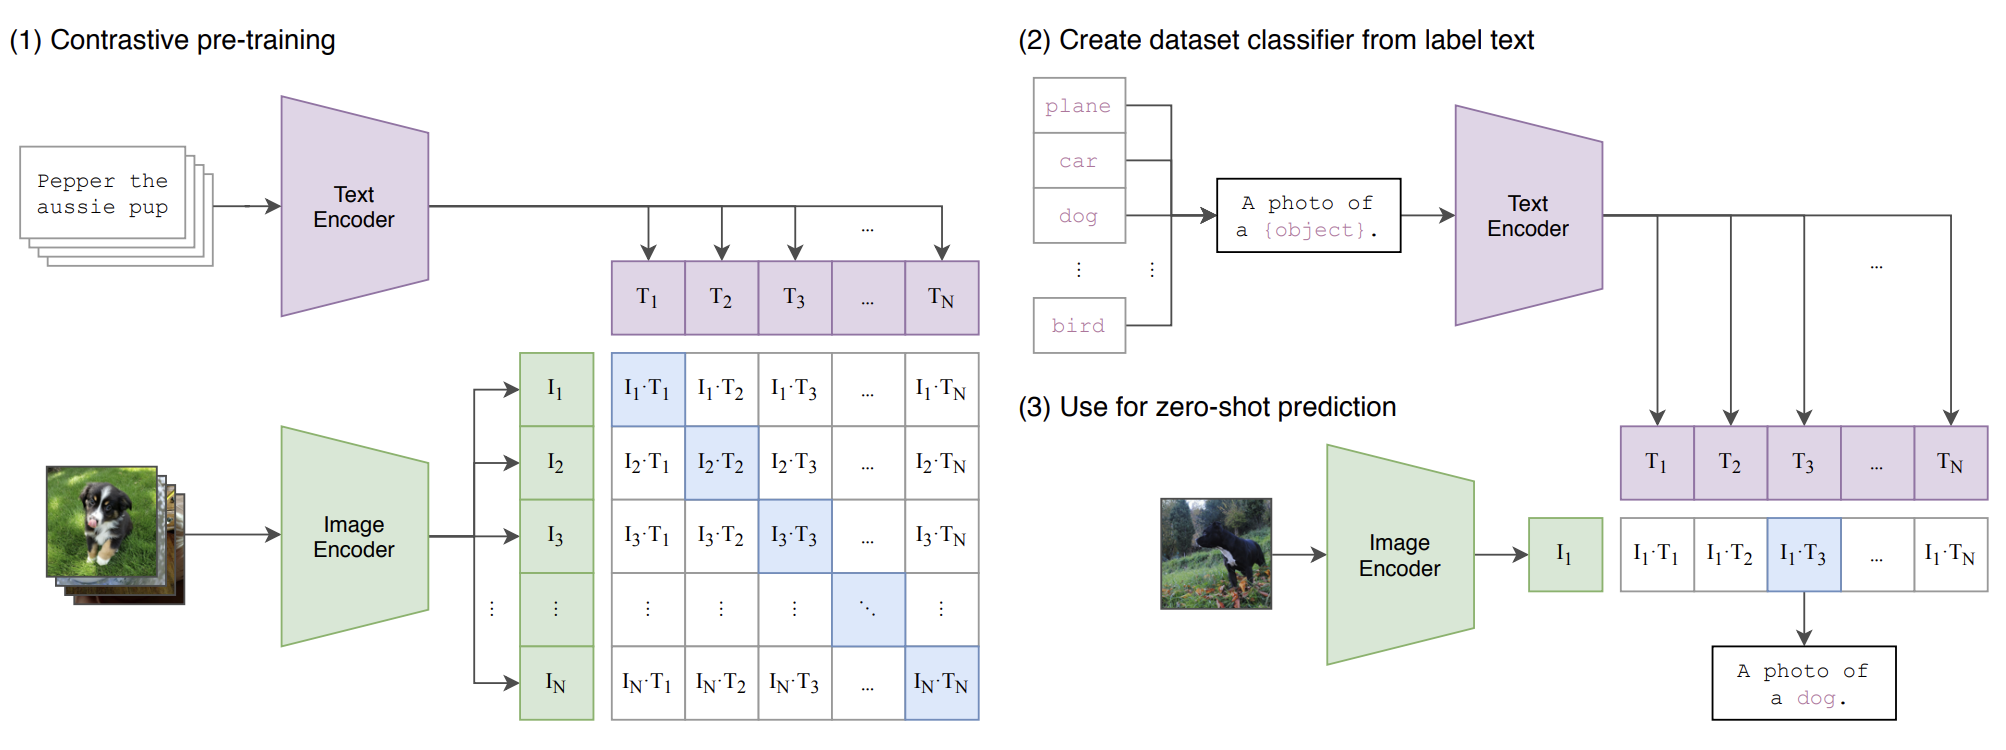
\includegraphics[width=0.7\textwidth]{images/diffusion_models/stable_diffusion/clip.png}
    \caption{(1) Contrastive pre-training stage of a CLIP model (training stage). (2) and (3): after the model has been pre-trained, its used as a zero-shot image classifier \cite{openai_clip}.}
    \label{fig:openai_clip}
\end{figure}

In figure \ref{fig:openai_clip},  $I_1, ..., I_N$ are the images, and $T_1, ..., T_N$ are the text prompts. The output is a \textbf{matrix of similarity scores} between the images and the text descriptions. Ideally in the matrix diagonal we get high similarity score (1) indicating high text-image alignment, and all other entries ideally should have low similarity score (0), indicating mismatch in text-image alignment.

The CLIP network is compromised of:

\begin{itemize}
    \item \textbf{Image encoder}: converts images to image embeddings.Its typically a vision transformer (ViT) \cite{vision_transformer} (appendix \ref{appendix:vision_transformer}) or a ResNet \cite{resnet} model.
    \item \textbf{Text encoder}: converts text descriptions to text embeddings. Its typically implemented as a transformer, or less common as a continuous bag of words \cite{cbow_word2vec} (known as Word2Vec model by Google, 2013 \cite{cbow_word2vec}).
    \item \textbf{Training objective}: the CLIP model is trained using a contrastive objective (commonly referred to as CLIP objective), where the goal is to minimize the cosine distance in the main diagonal and maximize the distance for non-matching image-text pairs (off diagonal).
\end{itemize}





















\subsection{DDIM Sampler}
\label{subsec:ddim_sampler}

\begin{figure}[ht]
    \centering
    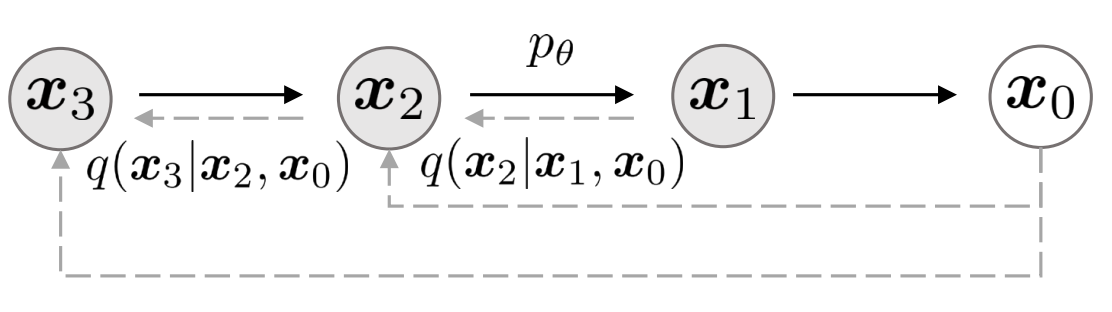
\includegraphics[width=0.4\textwidth]{images/diffusion_models/stable_diffusion/ddim_non_markov_process.png}
    \caption{Non-Markovian inference in DDIM. Each step depends on both the previous step and the initial state $x_0$ \cite{ddim}.}
    \label{fig:ddim_non_markov_process}
\end{figure}

Denoising Diffusion Implicit Models (DDIM), introduced in \cite{ddim}, provide an \textbf{efficient sampling method} for diffusion models, offering improvements over the traditional Denoising Diffusion Probabilistic Models (DDPM) \cite{ddpm}. Unlike DDPM sampler, which uses a fixed noise schedule and stochastic sampling, DDIM introduces a flexible noise schedule and a \textbf{deterministic sampling process}, enabling faster inference (10x to 50x speedup compared to DDPM \cite{ddim}).

Key points \& main contributions of the DDIM paper:

\begin{itemize}
    \item \textbf{Non-Markovian process}: As illustrated in figure \ref{fig:ddim_non_markov_process}, DDIM's reverse process depends on both the previous step and the initial state $x_0$, forming a deterministic trajectory through the latent space.
    \item \textbf{Implicit probabilistic model}: DDIM is an implicit probabilistic model, meaning that it doesn't directly model the joint distribution of the data but rather models the conditional distribution of the data given the noise.
    \item \textbf{Deterministic sampling}: Noise is removed directly in a controlled manner, skipping unnecessary diffusion steps and avoiding stochasticity.
    \item \textbf{Training objective}: DDIM uses the same training objective as DDPM and no modifications are needed.
    \item \textbf{Sampling process}: Sampling in DDIM involves sampling from the prior distribution and then iteratively sampling from the conditional distributions. This process is faster than traditional diffusion models because it doesn't require simulating the entire Markov chain.
\end{itemize}

DDIM introduces a generalized forward process:

\[
q_\sigma (x_{t-1} | x_t, x_0) = \mathcal{N} \left( \sqrt{\alpha_{t-1}} x_0 + \sqrt{1 - \alpha_{t-1} - \sigma_t^2} \cdot \frac{x_t - \sqrt{\alpha_t} x_0}{\sqrt{1 - \alpha_t}}, \sigma_t^2 I \right),
\]

where $\sigma \in \mathbb{R}^T_{\geq 0}$ controls the stochasticity of the forward process:
- For $\sigma \rightarrow 0$, the process becomes fully deterministic, as $x_{t-1}$ is uniquely determined by $x_t$ and $x_0$.

\begin{figure}
    \centering
    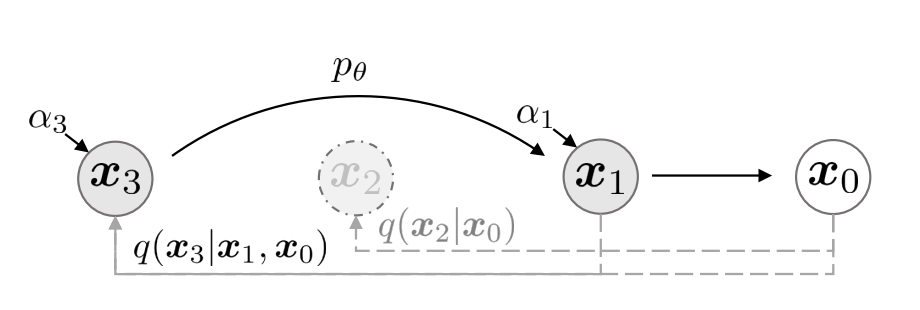
\includegraphics[width=0.5\textwidth]{images/diffusion_models/stable_diffusion/ddim_sampling_process.png}
    \caption{DDIM sampling \cite{ddim}. In the figure, $x_3$ depends only on $x_0$ and $x_1$ (and not $x_2$). This process can be generalized to all subsets of steps.}
    \label{fig:ddim_sampling_process}
\end{figure}

\begin{figure}
    \centering
    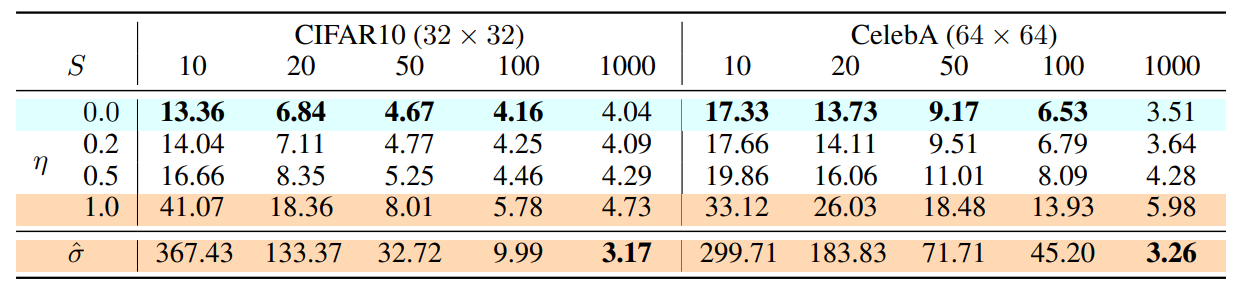
\includegraphics[width=0.7\textwidth]{images/diffusion_models/stable_diffusion/ddim_sample_quality.png}
    \caption{DDIM gives almost the same sample quality compared to DDPM sampler, and requires less compute since we skip some of the diffusion steps. The stochasticity of the model is controlled by $\eta$ \cite{ddim}.}
    \label{fig:ddim_sample_quality}
\end{figure}

In figure \ref{fig:ddim_sample_quality} DDIM gives almost the same sample quality in FID metric (equation \ref{eq:fid_score}, lower is better) compared to DDPM and require much less compute. The experiment was done on CIFAR10 and CelebA datasets, with 10,20,50,100,1000 steps. When $\eta = 0$ (blue) the model is deterministic (DDIM process), and when $\eta = 1$ (orange) the model is stochastic (DDPM process).















\subsection{Training}

Stable Diffusion is trained in CFG manner (section \ref{subsec:classifier_free_diffusion_guidance}).

The authors made simplified loss objective which predicts the noise removal process at each step:

\[
    L_{\text{DM}} = \mathbb{E}_{x, \epsilon \sim \mathcal{N} (0, 1), t} \left[ \Vert \epsilon - \epsilon_\theta(x_t, t) \Vert _2^2 \right]
\]

This loss function is similar to the loss function of DDPM (equation \ref{eq:ddpm_loss}).













\subsection{Implementation of $\tau_\theta$ transformer for conditional LDMs}

The researchers provded high level overview of the implementation of the conditional encoder for text $\tau_\theta$, consisted of $N$ transformer blocks:

\begin{align*}
    &\zeta \leftarrow \text{TokEmb}(y) + \text{PosEmb}(y) \\
    &\text{for } i = 1, \ldots, N : \\
        &\hspace{1cm} \zeta_1 \leftarrow \text{LayerNorm}(\zeta) \\
        &\hspace{1cm} \zeta_2 \leftarrow \text{MultiHeadSelfAttention}(\zeta_1) + \zeta \\
        &\hspace{1cm} \zeta_3 \leftarrow \text{LayerNorm}(\zeta_2) \\
        &\hspace{1cm} \zeta \leftarrow \text{MLP}(\zeta_3) + \zeta_2 \\
    &\zeta \leftarrow \text{LayerNorm}(\zeta)
\end{align*}

where:

\begin{itemize}
    \item $\zeta := \tau_\theta(y)$ is the unmasked transformer output (the transformer processes the tokenized version of $y$), which is then used in the cross-attention mechanism of the stable diffusion model.
    \item TokEmb is the token embeddings.
    \item PosEmb is the positional embeddings.
    \item LayerNorm is the layer normalization (appendix \ref{appendix:blocks_norm}).
    \item MultiHeadSelfAttention is the multi-head self-attention mechanism (appendix \ref{appendix:attention}).
    \item and MLP is the multi-layer perceptron (appendix \ref{appendix:blocks}) block.
\end{itemize}


\begin{figure}[h]
    \centering
    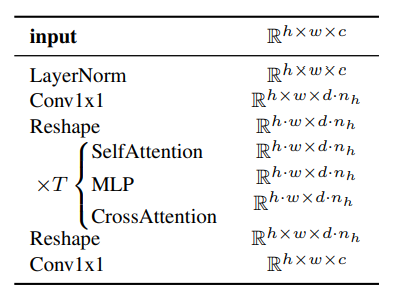
\includegraphics[width=0.3\textwidth]{images/diffusion_models/stable_diffusion/transformer_block.png}
    \caption{Architecture of the transformer block used in Stable Diffusion, where $n_h$ denotes the number of attention heads and $d$ the dimensionality per head \cite{stable_diffusion}.}
\end{figure}











\subsection{Details on Autoencoders Models}

In the stable diffusion paper, the researchers trained the pixel-space encoder $\varepsilon$ and the decoder $\mathcal{D}$ in adversarial manner (adversarial loss \cite{vqgan}). A patch-based discriminator $D_\psi$ is optimized to differentiate the original image from reconstructed image $\mathcal{D} (\varepsilon (x))$ which helps guide the autoencoder.

In addition, the researchers used two methods for regularizing the latent space:

\begin{itemize}
    \item \textbf{KL-divergence regularization}: similar to VAEs where the latent space is a distribution, the KL regularization objective pushes the latent space to be close to a standard normal distribution.
    \item \textbf{VQ regularization}: similar to VQ-GAN and VQ-VAE (sections \ref{vqgan} and \ref{vqvae}), the vector quantization regularization forces the latent space to be discrete, which can help the model to learn better by using a codebook $\mathcal{Z}$.
\end{itemize}

They factorized the KL term by a factor of $\sim 10^{-6}$, and in VQ regularization they used a big codebook.

The full loss objective to train the autoencoder model $(\varepsilon, \mathcal{D})$ is given by:

\begin{equation*}
    L_{\text{Autoencoder}} = \min_{\varepsilon, \mathcal{D}} \max_{\psi} \left( L_{\text{rec}} (x, \mathcal{D} (\varepsilon (x))) - L_{\text{adv}} (\mathcal{D} \varepsilon (x)) + \log \mathcal{D}_\psi (x) + L_{\text{reg}} (x; \varepsilon, \mathcal{D}) \right)
\end{equation*}


















\subsection{Experiments}

The researchers conducted several experiments with different LDM downsampling factors, and compared the results with other state-of-the-art models (DALL-E, VQGAN, StyleGAN, ProjectedGAN, CogView, GLIDE, and others).

\begin{figure}
    \centering
    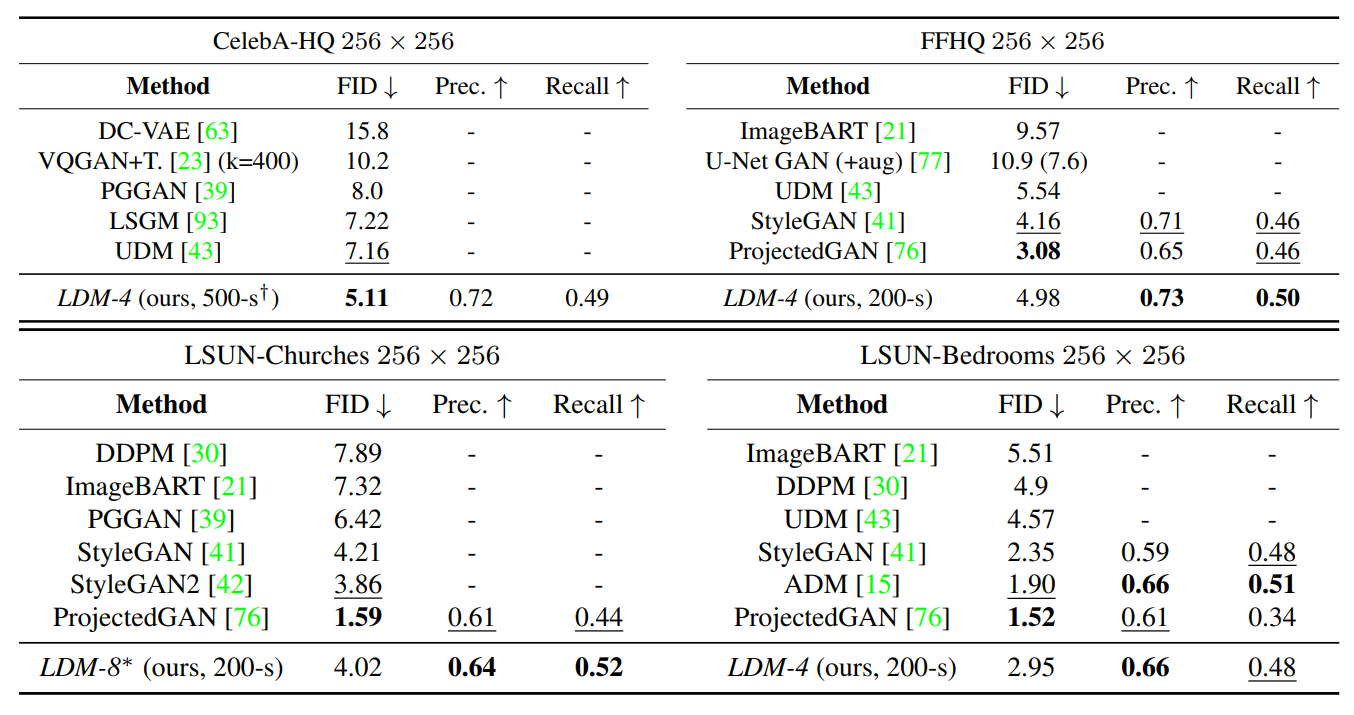
\includegraphics[width=0.7\textwidth]{images/diffusion_models/stable_diffusion/experiments_1.png}
    \caption{Unconditional image synthesis evaluation between LDM (Stable Diffusion) and other models across 4 datasets \cite{stable_diffusion}.}
    \label{fig:stable_diffusion_experiments_unconditional}
\end{figure}

In figure \ref{fig:stable_diffusion_experiments_unconditional} we clearly see that LDM outperforms most of the state-of-the-art models, across multiple metrics and datasets. $\dagger$ refers to the DDIM sampler steps (500 top-left, 200 top-right, 200 bottom-left, 200 bottom-right).

\begin{figure}
    \centering
    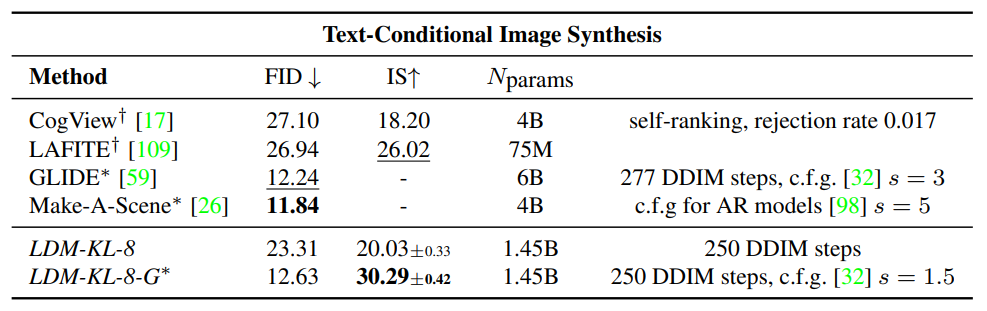
\includegraphics[width=0.6\textwidth]{images/diffusion_models/stable_diffusion/experiments_2.png}
    \caption{Evaluation of text-conditioned image synthesis on MS-COCO dataset. LDM with 250-DDIM steps is on par with the most recent diffusion and autoregressive methods, \textbf{while using significantly less parameters} (1.45 billion) \cite{stable_diffusion}.}
\end{figure}

For text-to-image tasks, the researchers trained a 1.45B parameters model conditioned on language prompts on LAION-400M dataset. The model uses \textbf{BERT-Tokenizer} \footnote{Its important to note that the researchers used the BERT text tokenizer in the paper, however, in the \href{https://github.com/CompVis/latent-diffusion}{offical released implementation of Stable Diffusion} they used CLIP tokenizer. The reason is that in the Imagen paper \cite{imagen}, the researchers found out that using larger language models had more impact on generated image quality than larger image generation components. This fact is shown in figure \ref{fig:imagen_clip_score_bigger_llm}.} \cite{bert} and implement $\tau_\theta$ (the domain-specific conditional encoder) as a transformer.

\begin{figure}
    \centering
    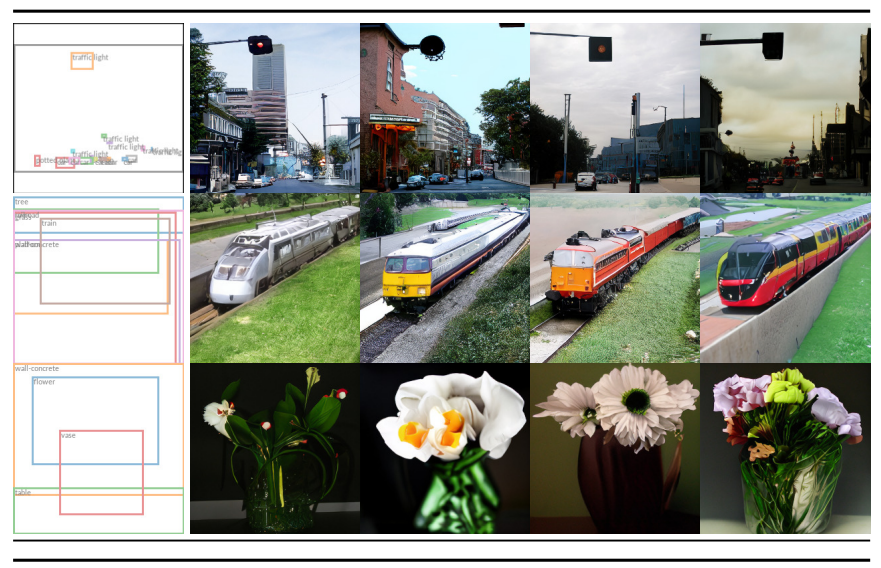
\includegraphics[width=0.5\textwidth]{images/diffusion_models/stable_diffusion/experiments_3.png}
    \caption{Samples of Stable Diffusion conditioned on semantic layouts \cite{stable_diffusion}.}
    \label{fig:stable_diffusion_experiments_semantic_layouts}
\end{figure}

For semantic layouts, the model is trained to synthesis images based on semantic layouts from the OpenImages dataset and fine-tuned on COCO dataset (figure \ref{fig:stable_diffusion_experiments_semantic_layouts}).

In figure \ref{fig:imagen_scaling_encoder_more_impactful_than_unet_scaling}, which is from Imagen paper \cite{imagen}, we see that using larger text encoder has more impact on image quality than larger image generation components (like the U-Net). This is why in Stable Diffusion, the implementation uses CLIP tokenizer instead of BERT tokenizer (which was originally used in the paper).

\section{Imagen}
\label{sec:imagen}

Imagen \cite{imagen} is a T2I diffusion model that builds on the power of large transformer language models \cite{transformer} (LLMs) to generate high-fidelity images. The combination of diffusion and LLMs have shown remarkable outputs. 

The paper has 5 main key takeaways and observations:

\begin{enumerate}
    \item \textbf{Effectiveness of large frozen text encoders}: one of the main observation in the paper that a large frozen language model trained only on text data have a significant impact on the fidelity of generated images compared to increasing the parameters of the diffusion image model. Scaling the language model is easy, since unlabeled text data is abundant and available on the internet.
    \item \textbf{Dynamic thresholding}: is a new sampling technique (section \ref{subsec:imagen_diffusion_guidance_weight}) that improves image fidelity and text-image alignment, which improves upon static thresholding.
    \item \textbf{Effective U-Net}: a new U-Net architecture that is simpler and more memory efficient.
    \item \textbf{COCO FID score of 7.27}: imagen achieved a new state-of-the-art COCO FID score of 7.27, which outperforms all other previous works.
    \item \textbf{DrawBench}: a new human evaluation benchmark for T2I task. Imagen outperforms all other works, including DALL-E \cite{dalle}, VQ-GAN+CLIP \cite{vqgan_clip}, LDM \cite{stable_diffusion}, GLIDE \cite{glide}, and DALL-E 2 \cite{dalle_2}.
\end{enumerate}



















\subsection{Text-to-Text Transfer Transformer (T5)}
\label{subsec:t5}

\textbf{T}ext-\textbf{t}o-\textbf{T}ext \textbf{T}ransfer \textbf{T}ransformer (T5) \cite{t5_model} by Google Research is a language model that treats tasks as a text-to-text (T2T) problems. For example we could prompt the model:

\begin{itemize}
    \item \textbf{Summarization}: "Translate the following text to a summary: ..."
    \item \textbf{Translation}: "Translate the following text from English to French: ..."
    \item \textbf{Text classification}: "Classify the following text into one of the following categories: ..."
    \item \textbf{Question answering}: "Answer the following question: ..."
\end{itemize}

as well as other T2T tasks. In short, this knowledge can be viewed as developing a 'general-purpose' model that can understand text, instead of explicitly training the model to complete the specific downstream task.

The T5 model is open-source and was trained on large corpora of textual data. The base version of the model (T5-base) consists of 220 million parameters, while the largest version of the model (T5-XXL) consists of \textbf{11 billion parameters}. In the context of Imagen, \textbf{the Imagen model uses a frozen version of T5-XXL model} to encode conditional text prompts.

\textbf{Pre-training}: Unsupervised learning is appealing because unlabeled text data is abundant and available on the Internet. For example, the Common Crawl project \cite{common_crawl_project} is a non-profit organization that crawls the internet and provides free access to its achieved datasets to the public. A lot of research has been done on LLM models on large scale datasets, and the consensus is that \textbf{the larger the dataset, the better the model performs} \cite{radford2019language} \cite{jozefowicz2016exploring} \cite{hestness2017deep}. The T5 models were trained on the "Colossal Clean Crawled Corpus" (C4) dataset, which consists of 750GB of English text data scraped from the web.

\textbf{The training objective} of T5 model is called \textbf{span corruption}, which is stronger version of \textbf{masked language modeling}. Given a sentence, some words and some contiguous words are masked (in masked language modeling, only single words are masked), and the model should predict those words. For example: "Thank you for inviting me to your party last week", where the masked words are "for inviting" and "last". And the model should predict those words in the following sentence: "Thank you [MASKED] me to your party [MASKED] week". The model should learn to reconstruct the missing tokens.

\begin{figure}[h]
    \centering
    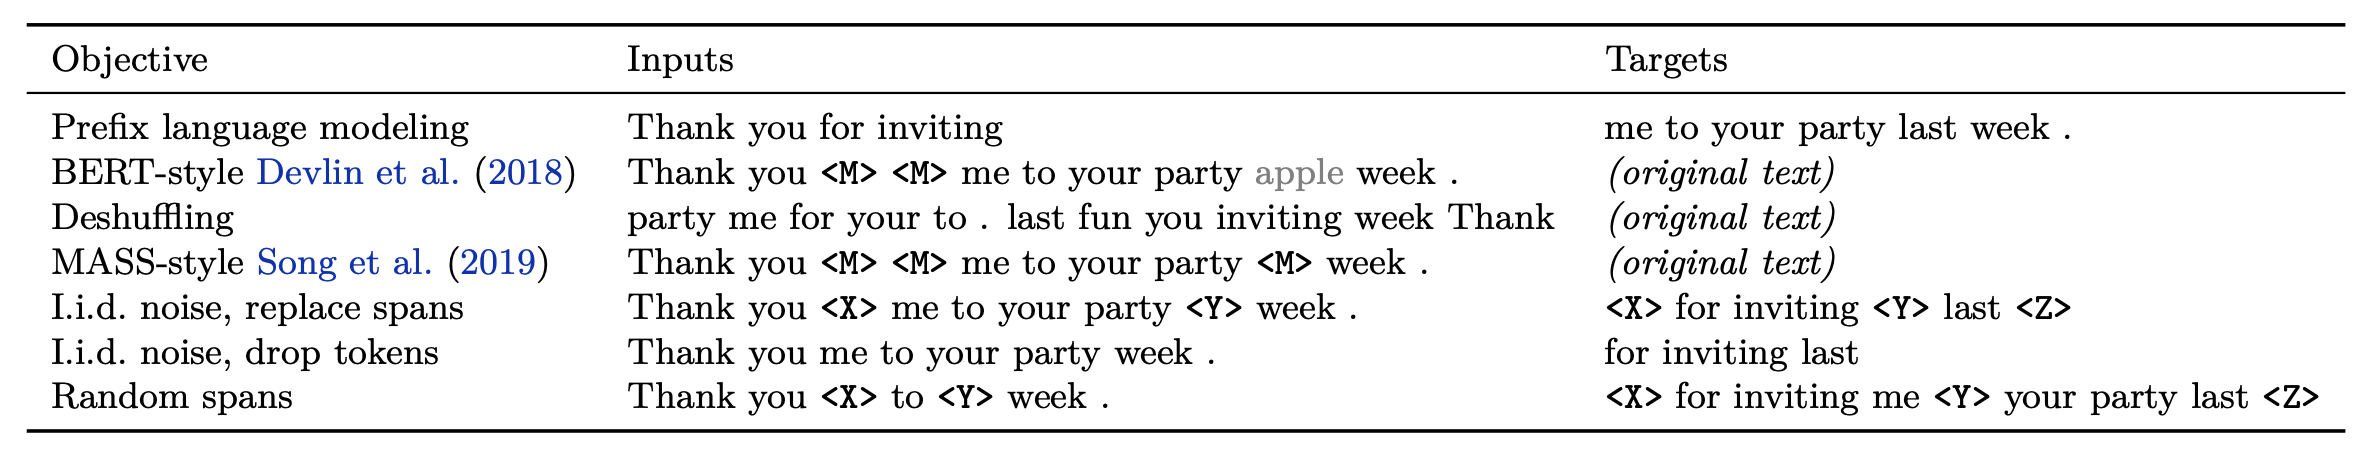
\includegraphics[width=1\textwidth]{images/imagen/t5_objectives.png}
    \caption{Mask modeling in T5 \cite{t5_model}.}
    \label{fig:t5_objectives}
\end{figure}

In figure \ref{fig:t5_objectives} \textless M\textgreater\ denotes shared mask token (the same mask token is used to represent all masked positions in the input). \textless X\textgreater, \textless Y\textgreater, and \textless Z\textgreater\ denote sentinel tokens which have unique token IDs; they mark specific masked positions that the model should reconstruct.















\subsection{Pre-trained text encoders}

In Imagen \cite{imagen} the researchers explored some of the biggest and most advanced text encoders: \textbf{T5-XXL} \cite{t5_model}, \textbf{GPT} \cite{gpt} \cite{mingpt} \cite{gpt_another}, and \textbf{BERT} \cite{bert}. These LLMs were trained exclusively on text datasets, which are substantially larger compared to image-text pair datasets (as used in models like \textbf{CLIP}).

Freezing these models \footnote{When we freeze models we generally mean that some (or all) of the parameters of the model are not changed during training. How? When a layer is frozen during training, no gradient updates will occur for this layer. Gradients will still flow from frozen layer to non-frozen layer, it doesn't skip the backpropagation. It just passes the gradients from the next layer to the previous layer.} provides significant advantage over training them: less memory and compute costs.














\subsection{Diffusion guidance weight}
\label{subsec:imagen_diffusion_guidance_weight}

As described before (section \ref{subsec:classifier_free_diffusion_guidance}), there are two methods to increase sample quality with the tradeoff of diversity:

\begin{itemize}
    \item \textbf{Classifier guidance} uses a separate, pre-trained classifier model to guide the image generation process in diffusion models by adjusting the noise based on how closely the generated image matches a desired condition.
    
    \item \textbf{Classifier-free guidance} (CFG) removes the need for a separate classifier by training the diffusion model itself to optionally condition on the label or text input.
\end{itemize}

More formally, in CFG, sampling is performed weighting the conditional and unconditional signals:

\begin{equation}
    \underbrace{\tilde{\epsilon}_\theta (z_t, c)}_{\text{adj noise prediction}} = \underbrace{w \epsilon_\theta (z_t, c)}_{\text{conditional score}} + \underbrace{(1 - w) \epsilon_\theta (z_t)}_{\text{unconditional score}}
    \label{eq:classifier_free_guidance}
\end{equation}

where $\epsilon_\theta$ is the noise prediction with the learned parameters $\theta$, $w$ is the guidance weight, $c$ is the condition, and $z_t$ is the latent variable at timestep $t$.

Imagen depends on CFG for effective text conditioning. They found that increasing the guidance weight improves image-text alignment but reduces image fidelity. Its caused by \textbf{train-test mismatch}: looking at equation \ref{eq:classifier_free_guidance} if we set $w$ to 1, then we disable CFG, and then the model won't be trained on unconditional samples (only on conditional signals). This causes the model to generate outputs that exceed the noise prediction in the normalized range of [-1, 1]. And when iteratively applying the model to its own outputs at each step, errors caused by this mismatch accumulate, which causes unnatural artifacts in output images. When we set $w>1$ then it improves the model's image-text alignment, but damages image fidelity.

For this reason they investigated static thresholding and dynamic thresholding:

\textbf{Static thresholding} applies the clipping operation to force the $x$-prediction output to fit to the normalized range of [-1, 1]. However, static thresholding still result in over-saturated and less detailed images as the guidance weight approaches 1.

\textbf{Dynamic thresholding}: instead of clipping the $x$-prediction to the normalized range, it sets a dynamic threshold $s$ based on the distribution of absolute pixel values in the current $x$-prediction, allowing the threshold to adapt to the specific output of the model at that moment. In other words, if the pixel values are saturated (close to the [-1, 1] range), dynamic thresholding pushes them inwards by thresholding in the range [-$s$, $s$] and then dividing by $s$.

\begin{figure}
    \centering
    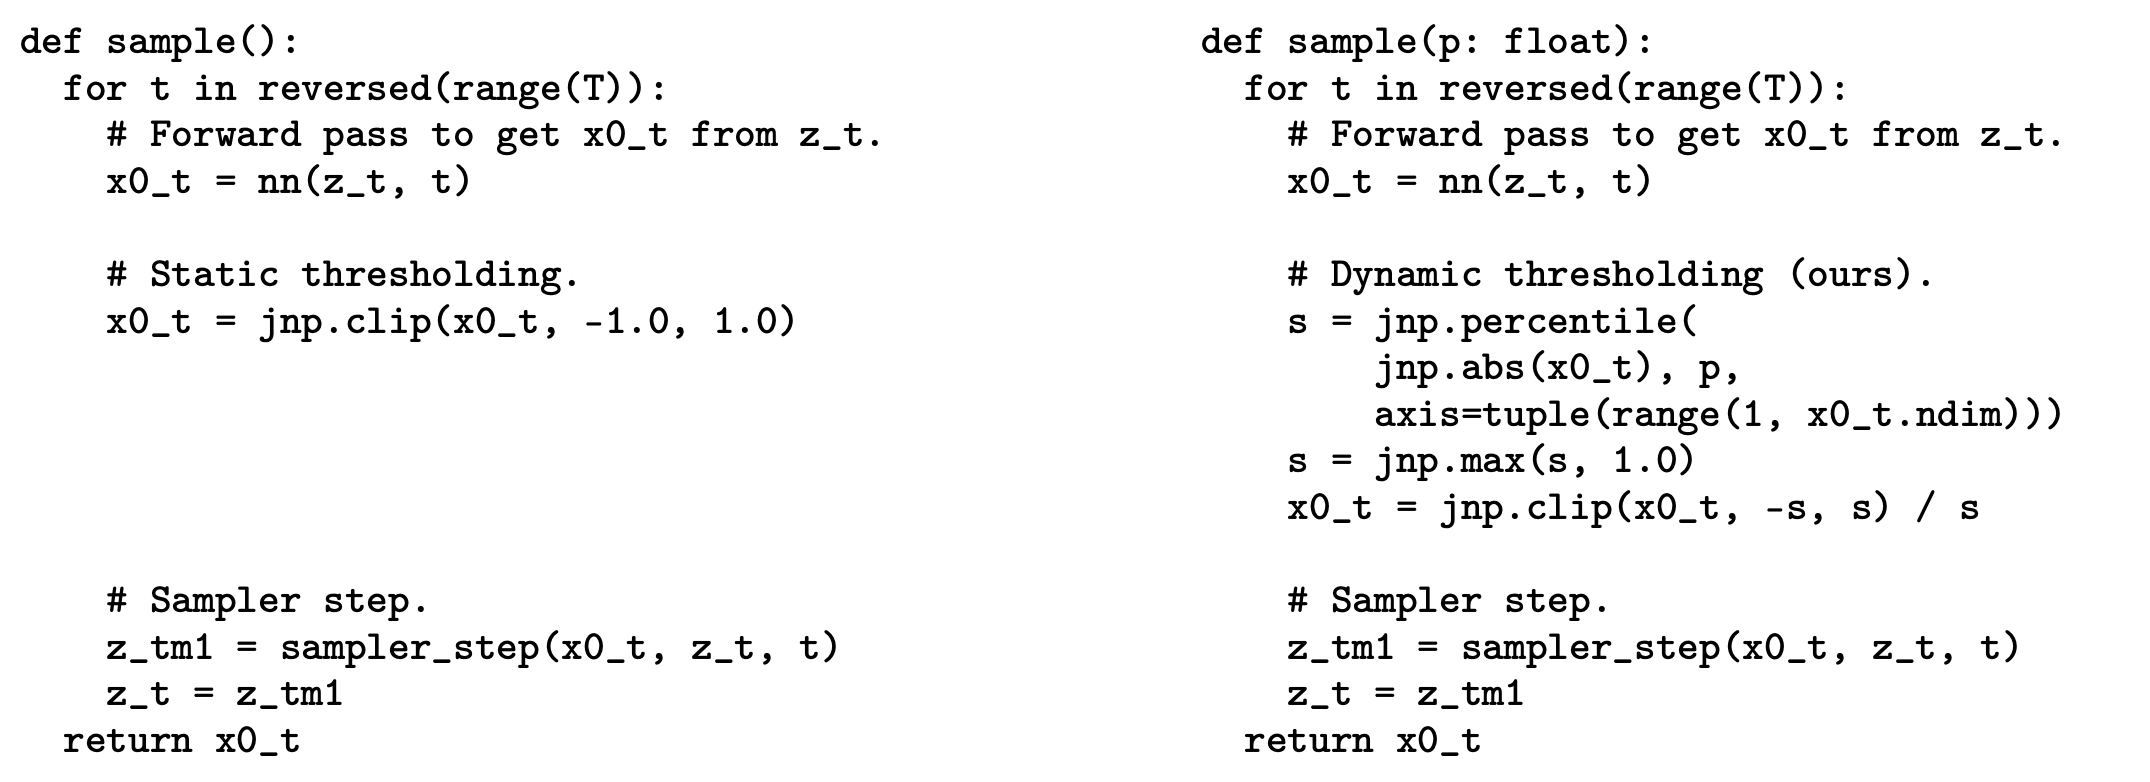
\includegraphics[width=0.7\textwidth]{images/imagen/static_dynamic_thresholding.png}
    \caption{Static (left) and dynamic (right) thresholding code implementation \cite{imagen}.}
    \label{fig:imagen_dynamic_thresholding}
\end{figure}

\begin{figure}
    \centering
    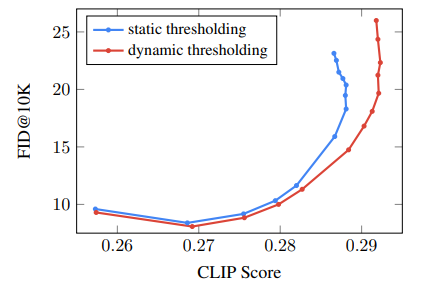
\includegraphics[width=0.4\textwidth]{images/imagen/static_vs_dynamic_thresholding.png}
    \caption{Static vs dynamic thresholding \cite{imagen}.}
    \label{fig:imagen_static_vs_dynamic_thresholding}
\end{figure}

The implementation of static and dynamic thresholding is shown in figure \ref{fig:imagen_dynamic_thresholding}. The impact of dynamic thresholding is shown in figure \ref{fig:imagen_static_vs_dynamic_thresholding} where its shown that dynamic thresholding produces samples with higher image-text alignment (CLIP) and fidelity (FID) compared to static thresholding.
















\subsection{Super-resolution via Repeated Refinement (SR3)}

\label{subsec:imagen_sr3}

In a 2021 paper \cite{sr3}, the Google Research team introduced a new super-resolution model based on diffusion process. \textbf{S}uper-resolution via \textbf{R}epeated \textbf{R}efinment (SR3) model upsamples in iterative manner, similar to reverse diffusion. It upsamples images from $64\times 64$ to $256\times 256$ and finally to $1024\times 1024$.

SR3 achieves close to a 50\% fool rate (47\%) \footnote{A 50\% fool rate means humans can't distinguish between a generated face image and an image of a real face.} on $16\times 16 \rightarrow 128\times 128$ faces, outperforming the previous state-of-the-art GAN models (FSRGAN and PULSE).

\textbf{Iterative refinement}: Given low-resolution image $x_{low}$ the model applies \textbf{bicubic interpolation} \footnote{Bicubic interpolation is a method for resizing images that uses the closest 4x4 pixels grid to estimate new values, resulting in smoother transitions (compared to nearest-neighbor or bilinear interpolation) and fewer visual artifacts.} to upscale the image to the target resolution to get high-resolution image $x$ and then concatenates $x$ with pure Gaussian noise $y_t \sim \mathcal{N} (0, I)$ channel-wise (see figure \ref{fig:sr3_architecture}). Then the U-Net iteratively refines the image $(x, y_t)$ by denoising. The output of a single refinement step (from the U-Net) is $y_{t-1}$. Then in the next refinement step, $x$ is concatenated with $y_{t-1}$ and the process is repeated until we reach $y_0$. The final output is a high-resolution image $y_0$. Note that both $x$ (after the upsampling), $y_i$ are all on same resolution / dimension (see figure \ref{fig:sr3_architecture}).

\textbf{The architecture of SR3} modified the diffusion U-Net: they replaced the original DDPM residual blocks with residual blocks from BigGAN \cite{biggan_deep}, rescaled skip connections by $\frac{1}{\sqrt{2}}$, increased the number of residual blocks, and increased the number of the channel multipliers \footnote{Channel multipliers in a U-Net are the scaling factors used to adjust the number of feature channels at different U-Net layers. In other words, they increased the depth of the features at the cost of decreasing resolution at the convolution layers (down convolution, up convolution layers)} at different resolutions.

% \begin{table}[h!]
%     \centering
%     \begin{tabular}{|l|m{8cm}|}
%         \hline
%         \textbf{Prior to Super Resolution} & \textbf{Limitations} \\ \hline
%         Autoregressive Models           & Computationally expensive; Limited resolution \\ \hline
%         Variational Autoencoder         & Sub-optimal sample quality \\ \hline
%         Generative Adversarial Network  & Difficult to optimize; Requires additional functions to prevent instability \\ \hline
%     \end{tabular}
%     \caption{Related works to super-resolution to SR3 and their limitations compared to SR3.}
% \end{table}


\begin{figure}
    \centering
    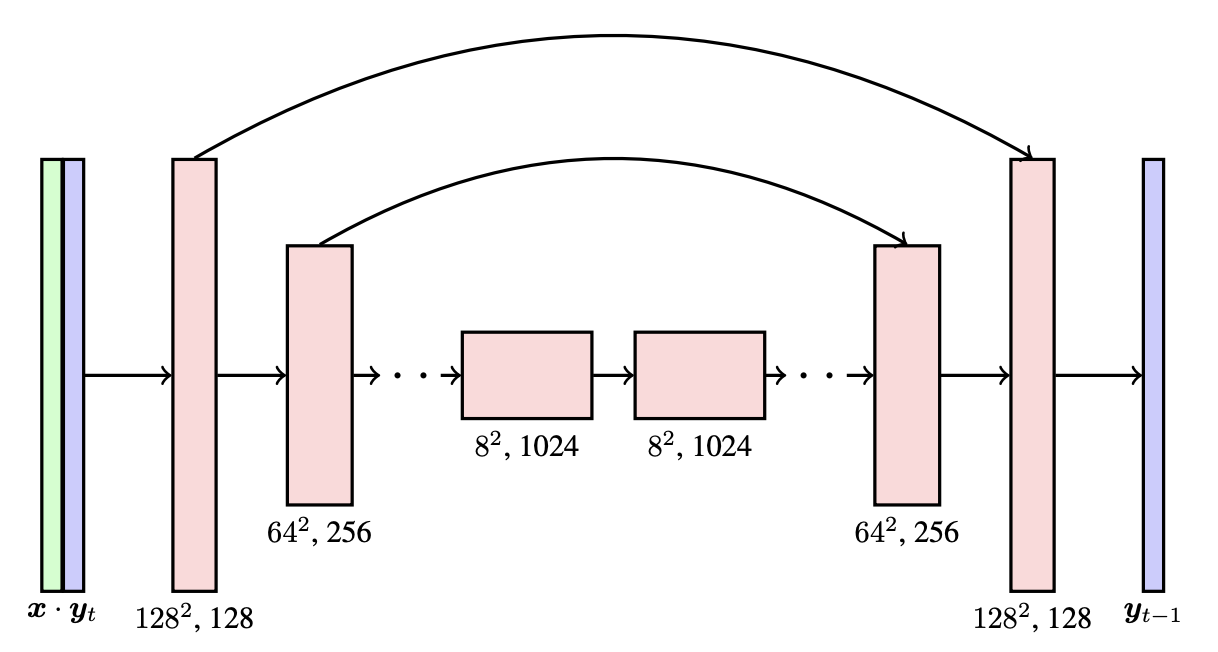
\includegraphics[width=0.5\textwidth]{images/imagen/sr3_architecture.png}
    \caption{SR3 $16\times 16 \rightarrow 128\times 128$ upsampling where $x$ is the input image, upscaled to the target resolution using bicubic interpolation, and then its concatenated with the noise $y$ \cite{sr3}.}
    \label{fig:sr3_architecture}
\end{figure}















\subsection{Cascaded diffusion models (CDMs)}

Cascaded diffusion models, introduced in a 2022 paper \cite{cascaded_diffusion_models} by Google Research, builds upon the SR3 paper \cite{sr3} and introduces a new method for super-resolution (SR) called Cascaded Diffusion Models (CDMs). CDMs use a base diffusion model that output image at low resolution, followed by a sequence (pipeline) of SR3 SR diffusion models that progressively upsamples until we reach the target resolution.

The CDM paper \cite{cascaded_diffusion_models} outperformed VQ-VAE 2 \cite{vqvae2} and BigGAN-deep \cite{biggan_deep} in SR task in FID metric on ImageNet dataset.

A big strength of CDMs is the ability to train and fine tune each model individually.

\textbf{Conditioning augmentation} is the main and critical part of the paper \cite{cascaded_diffusion_models}, which allows to generate images with higher FID, compared to without conditioning augmentation. Conditioning augmentation involves using data augmentation techniques on the low-resolution input image for each SR model in the cascaded pipeline. Augmentations such as Gaussian noise and Gaussian blur are applied to the  to the image which helps prevent each SR model from overfitting to the low-resolution input.

\begin{figure}
    \centering
    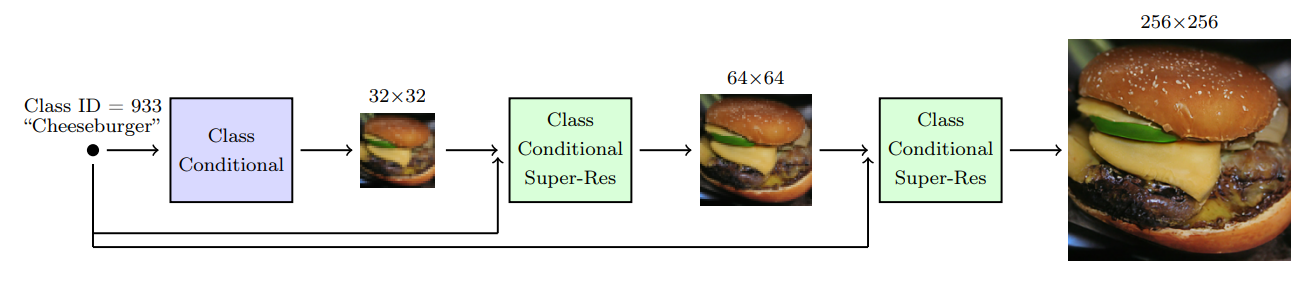
\includegraphics[width=0.7\textwidth]{images/imagen/cdm_architecture.png}
    \caption{CDM upsamples low-resolution image in the pipeline, conditioned on labels \cite{cascaded_diffusion_models}.}
    \label{fig:imagen_cdm_architecture}
\end{figure}























\subsection{Architecture}

An overview of Imagen architecture is shown in figure \ref{fig:imagen_architecture}.

The researchers conducted experiments with frozen LLMs such as BERT \cite{bert}, T5 \cite{t5_model}, and CLIP \cite{openai_clip} and found that humans prefer T5-XXL over CLIP. T5-XXL (T5-Extra Extra Large) text encoder maps text prompts to embeddings. The T5-XXL model has 11 billion parameters, and its the largest version of the T5 model. All the diffusion models are conditioned on the same text embeddings.

\textbf{Base model}: the base model is a $64\times 64$ T2I diffusion model. The network is conditioned on text embeddings (via cross-attention and layer normalization layers), as well as with diffusion timestep embeddings, similar to the class embedding conditioning in the CDM paper \cite{cascaded_diffusion_models}.

\textbf{SR models}: they used modified U-Net based on the improved DDPM paper \cite{openai_improved_ddpm} by OpenAI, By improving the U-Net they achieved 2-3x faster inference and convergence speed; they call this variant "\textbf{Efficient U-Net}". For the $256\times 256 \rightarrow 1024\times 1024$ SR model, they removed self-attention layers but keep the cross-attention layers.

\textbf{Efficient U-Net}: is a new U-Net architectural variant for SR models. Its more memory efficient and \textbf{2-3x faster in training and inference time}. There are several modifications to the U-Net architecture:

\begin{enumerate}
    \item \textbf{More residual blocks}: adding more residual blocks for lower resolutions, since lower-resolution images typically have more channels. They used 8 residual blocks at lower-resolution compared to typical 2-3 residual blocks used in a standard U-Net.
    \item \textbf{Scaling the skip connections} by $\frac{1}{\sqrt{2}}$, similar to SR3 \cite{sr3}, significantly improves convergence speed.
    \item \textbf{Reversing order of downsampling and upsampling blocks}: In a standard U-Net downsampling block, downsampling occurs after the convolution layers, and in the upsampling block, upsampling is done before the convolutions. They reverse this order for both blocks which significantly improves the forward pass without performance degradation.
\end{enumerate}

The efficient U-Net architecture for $64\times 64 \rightarrow 256\times 256$ is shown in figure \ref{fig:imagen_efficient_unet}.

\begin{figure}
    \centering
    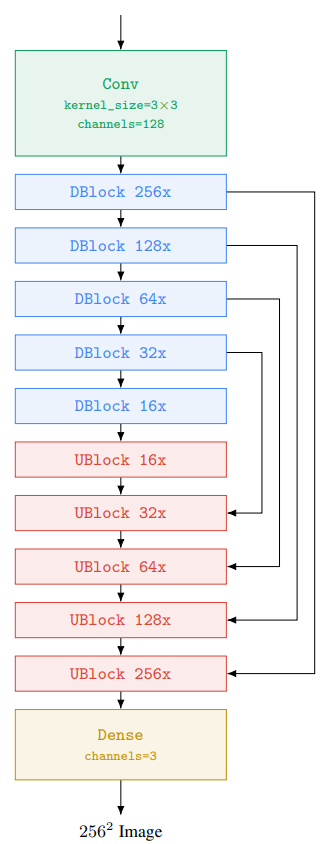
\includegraphics[width=0.25\textwidth]{images/imagen/efficient_unet.png}
    \caption{Efficient U-Net architecture for $64\times 64 \rightarrow 256\times 256$ SR model, proposed in Imagen \cite{imagen}.}
    \label{fig:imagen_efficient_unet}
\end{figure}

Similar to LDMs, Imagen also uses CFG \cite{classifier_free_guidance} (section \ref{subsec:classifier_free_diffusion_guidance}). Imagen depends critically on CFG for effective text conditioning.

\begin{figure}
    \centering
    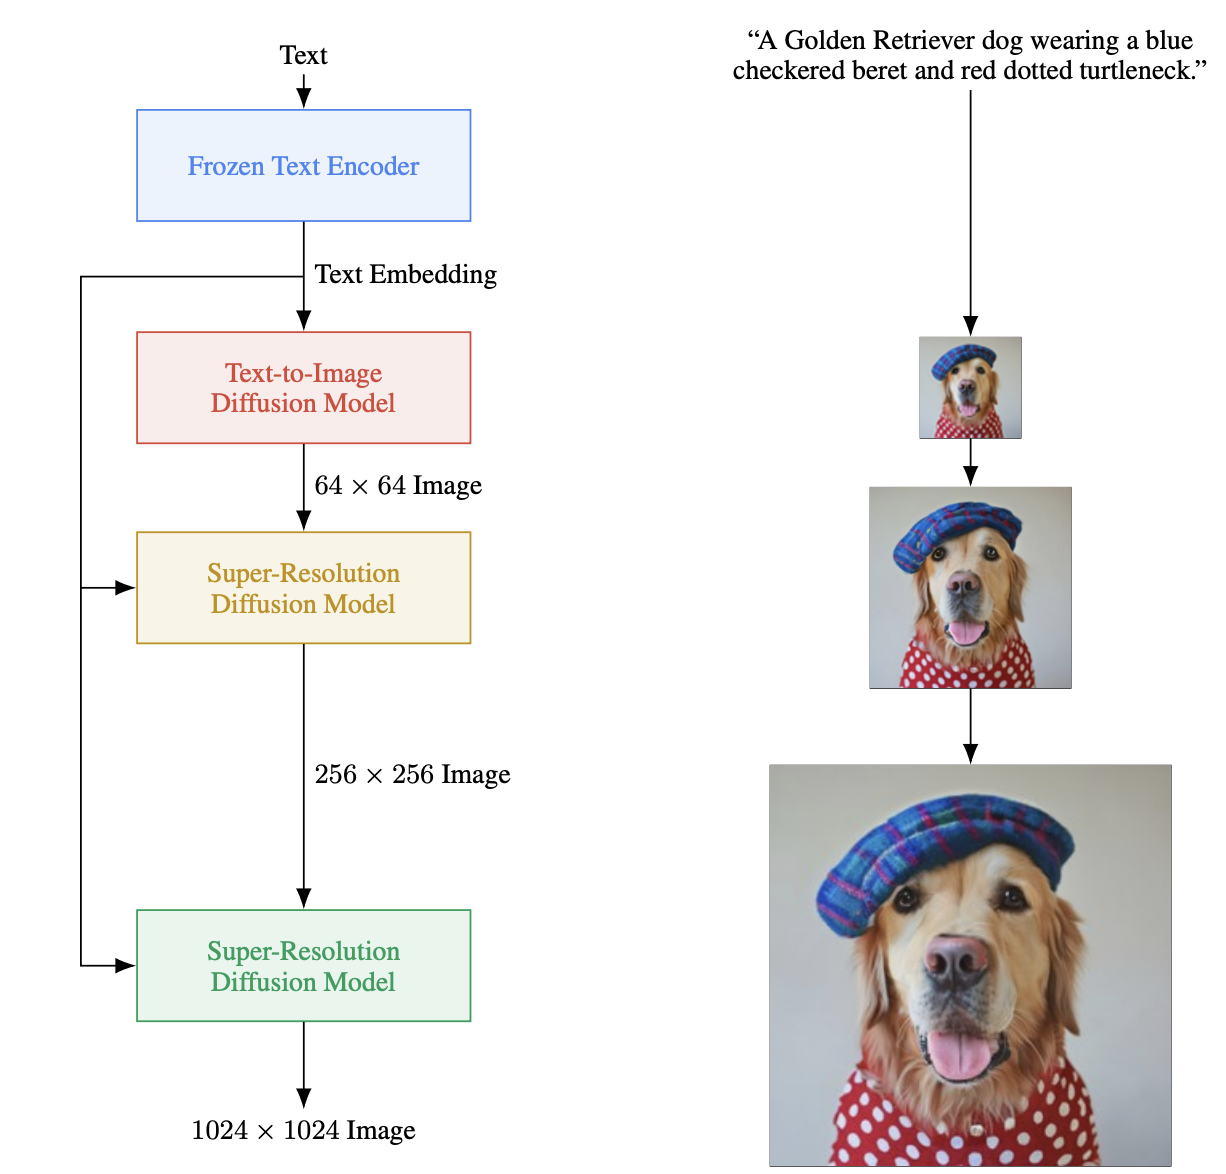
\includegraphics[width=0.5\textwidth]{images/imagen/architecture.png}
    \caption{Overview of Imagen architecture \cite{imagen}.}
    \label{fig:imagen_architecture}
\end{figure}

\textbf{Noise conditioning}: Imagen corrupts the $64\times 64$ image with Gaussian noise. The amount of noise is random at training but arbitrary at inference time. They control the amount of corruption with \textit{aug\_level}, and the SR model is conditioned on the augmentation level.

\textbf{Number of parameters}: the base T2I diffusion $64\times 64$ model has 2 billion parameters. The $64\times 64 \rightarrow 256\times 256$ SR model has 600 million parameters, and the $256\times 256 \rightarrow 1024\times 1024$ SR model has 400 million parameters. The size of the T5-XXL text encoder is 4.6 billion parameters.

\begin{figure}
    \centering
    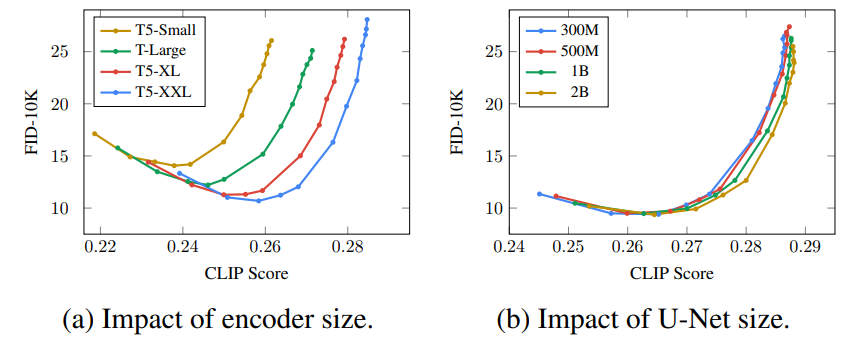
\includegraphics[width=0.75\textwidth]{images/imagen/encoder_vs_unet_size_impact.png}
    \caption{Scaling the encoder size is more impactful than scaling the U-Net size \cite{imagen}.}
    \label{fig:imagen_scaling_encoder_more_impactful_than_unet_scaling}
\end{figure}

\textbf{Scaling text encoder size is more important than U-Net size}: the researchers found that scaling the text encoder has significantly more impact than increasing U-Net size: see figure \ref{fig:imagen_scaling_encoder_more_impactful_than_unet_scaling}.



% DBlock, UBlock

\begin{figure}
    \centering
    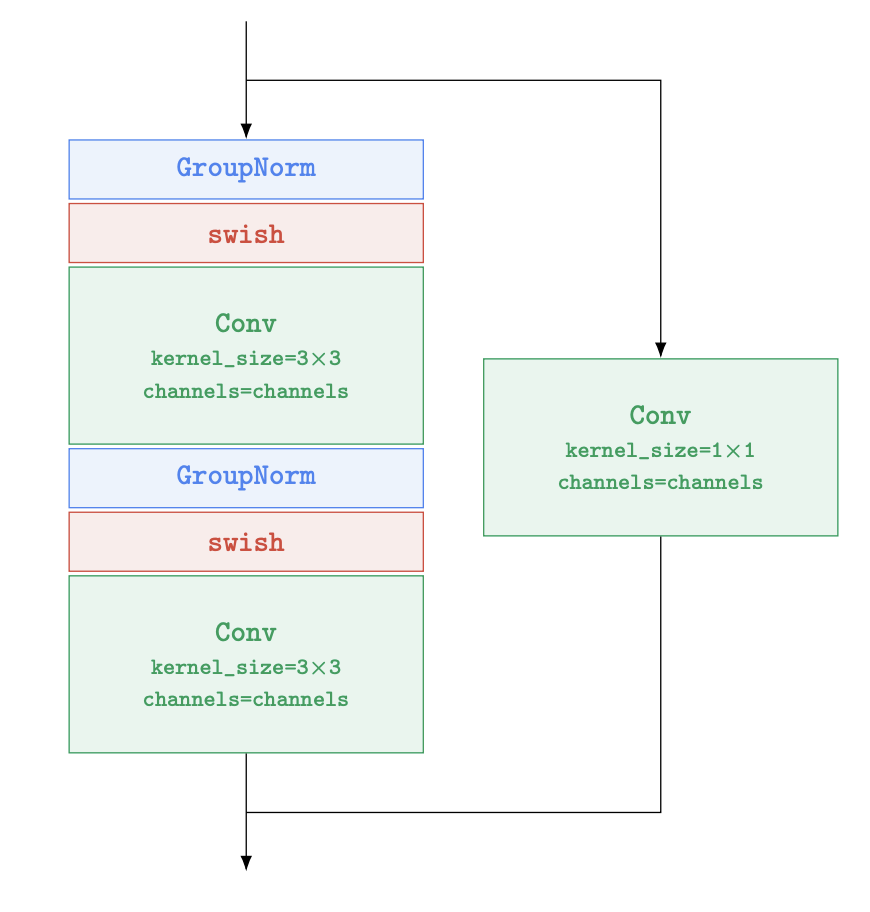
\includegraphics[width=0.35\textwidth]{images/appendix/imagen/unet_resnetblock.png}
    \caption{Imagen efficient U-Net \texttt{ResNetBlock} architecture \cite{imagen}.}
    \label{fig:imagen_resnetblock}
\end{figure}

In figure \ref{fig:imagen_resnetblock} we can see the \texttt{ResNetBlock} which is in use by both the \texttt{DBlock} and the \texttt{UBlock}. The only input of the \texttt{ResNetBlock} is the number of channels. The activation function is Swish (equation \ref{eq:appendix_activations_swish}). 

\begin{figure*}
    \centering
    \begin{subfigure}[b]{0.5\textwidth}   
        \centering 
        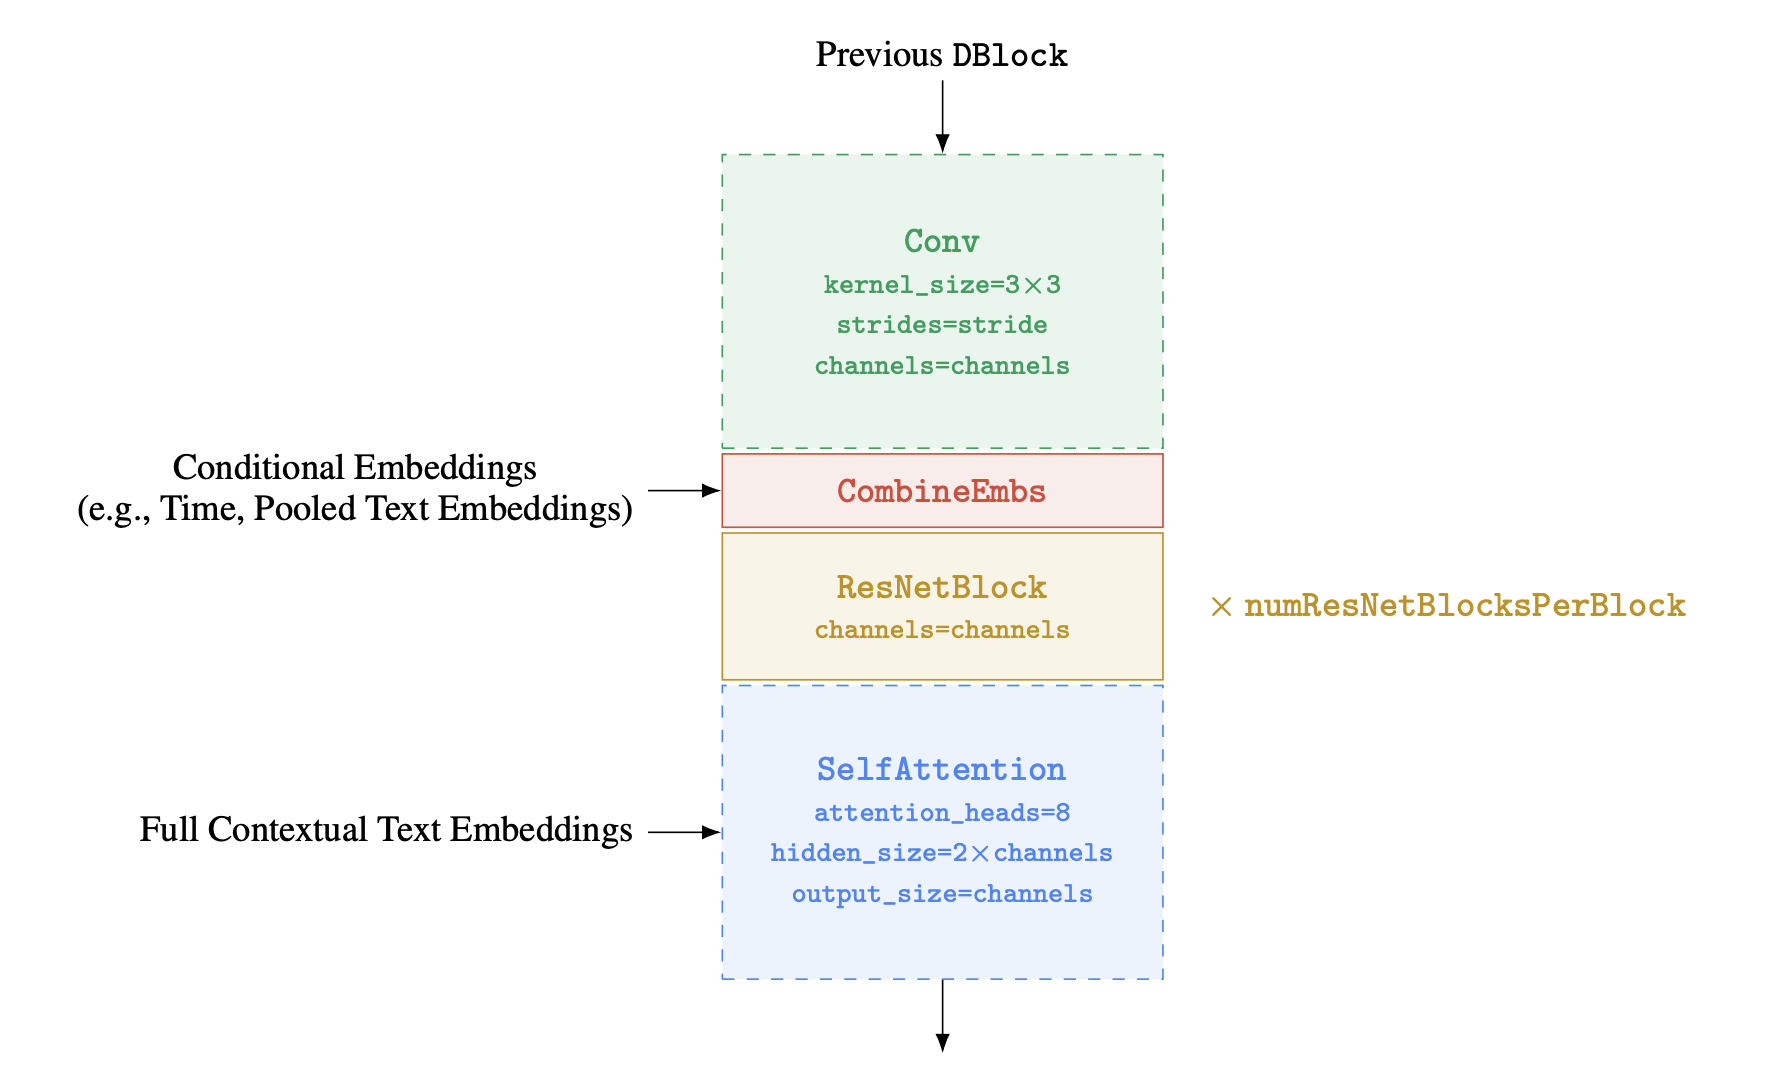
\includegraphics[width=\textwidth]{images/appendix/imagen/dblock.png}
        \caption[]%
        {{\small Imagen efficient U-Net \texttt{DBlock} architecture \cite{imagen}.}}
    \end{subfigure}
    \hfill
    \begin{subfigure}[b]{0.475\textwidth}
        \centering
        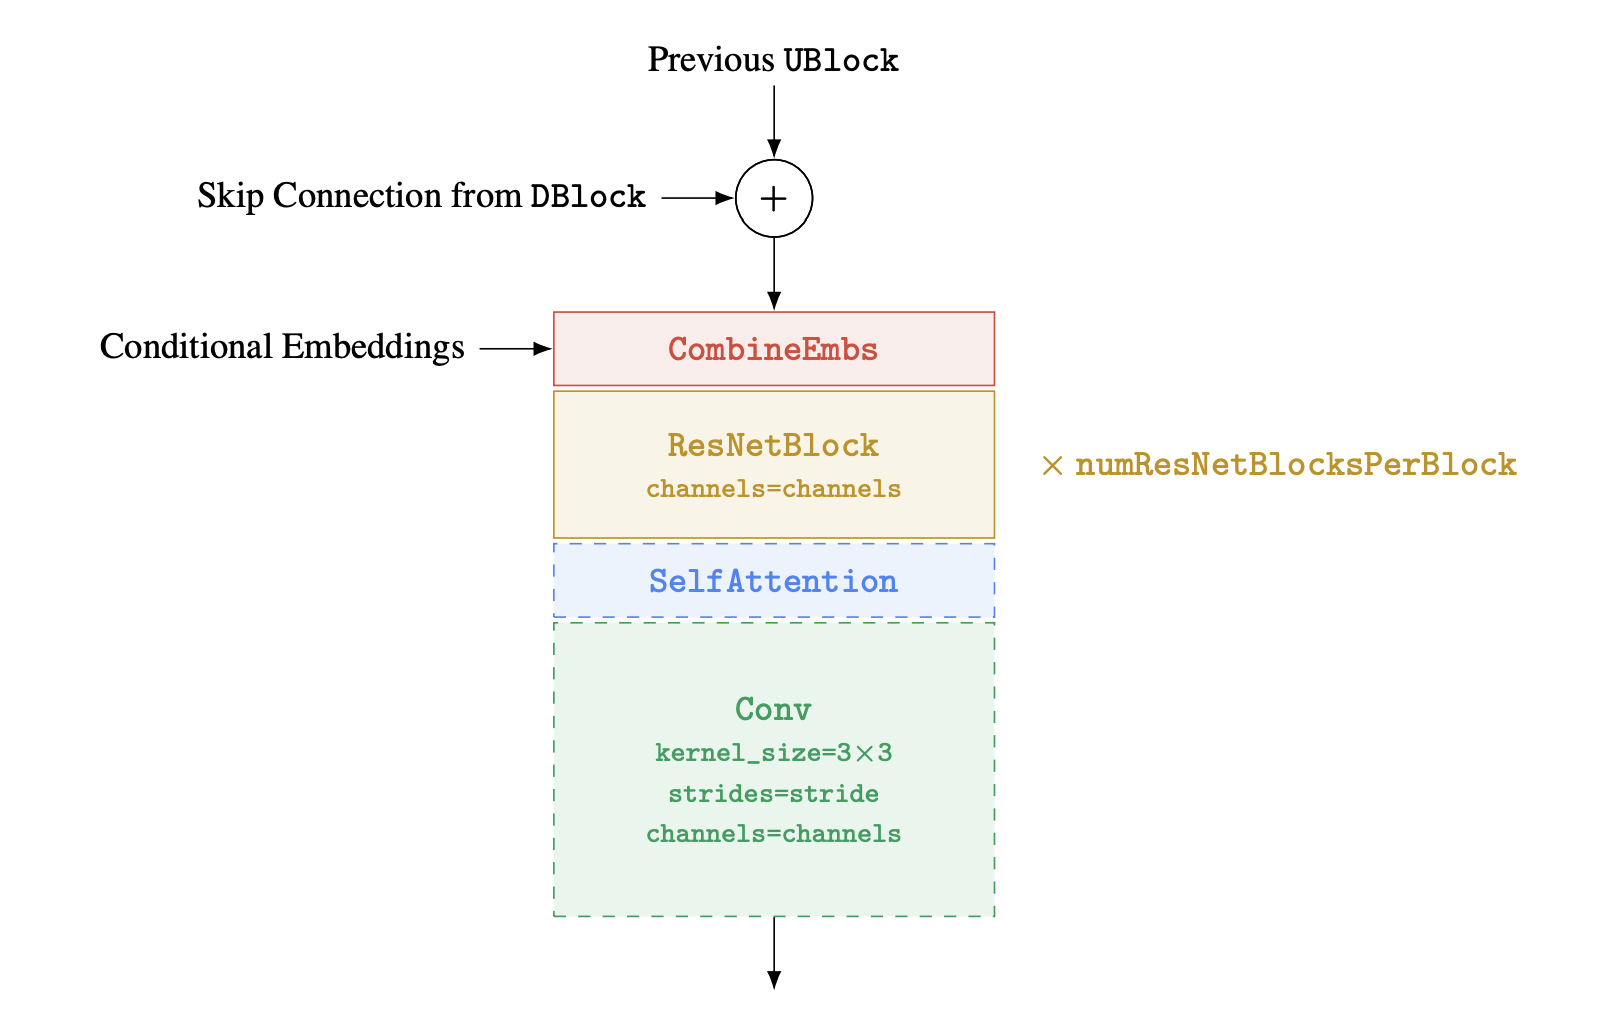
\includegraphics[width=\textwidth]{images/appendix/imagen/ublock.png}
        \caption[]%
        {{\small Imagen efficient U-Net \texttt{UBlock} architecture \cite{imagen}.}}
    \end{subfigure}
\end{figure*}















\subsection{DrawBench}

The COCO dataset \cite{coco_dataset} is a standard benchmark for evaluating T2I models. The standard performance metrics used are FID \cite{fid_score} which measure image fidelity (but is not fully aligned with perceptual quality \cite{perceptual_quality}), and CLIP score \cite{openai_clip} which measures image-text alignment (but is bad at counting objects in an image).

Due to these limitations, the researchers created new benchmark called \textbf{DrawBench} that uses human evaluation to assess image quality by asking the question "Which image is more photorealistic (looks more real)?" and text-image alignment by asking the question "Does the caption accurately describe the above image?". For both cases they used 200 randomly chosen image-caption pairs from COCO dataset.

\begin{figure}
    \centering
    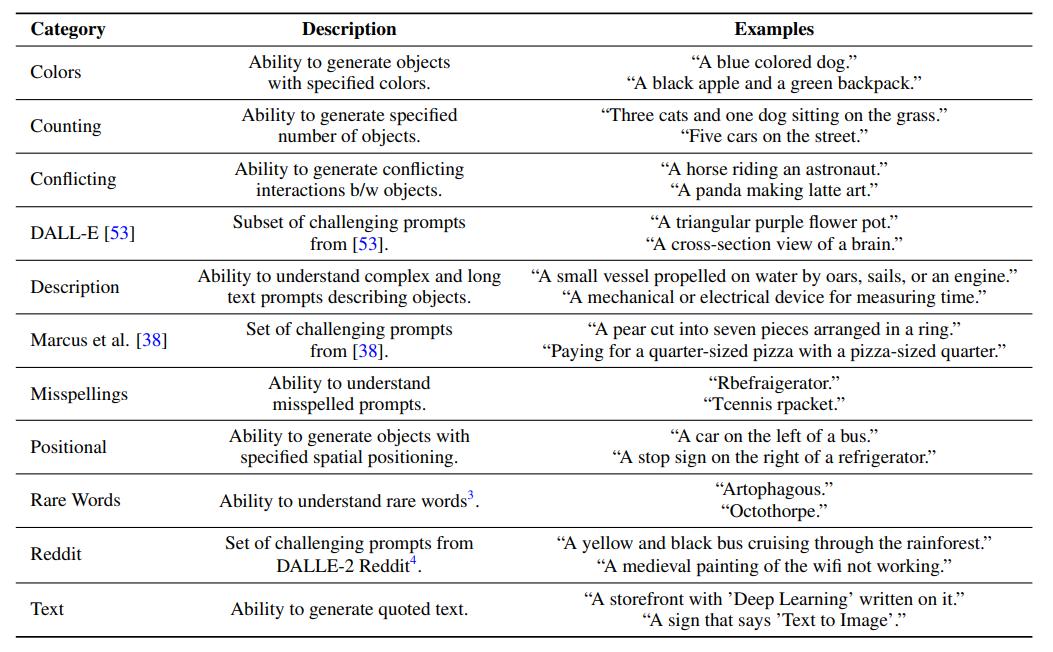
\includegraphics[width=0.6\textwidth]{images/imagen/drawbench_categories.png}
    \caption{Descriptions and examples of the 11 categories in DrawBench \cite{imagen}.}
    \label{fig:imagen_drawbench_categories}
\end{figure}

DrawBench has 11 categories of prompts which test different capabilities of models such as ability to render different colors, number of objects, spatial relations, text in the scene, and more. The prompts include long captions, rare words, and misspelled prompts. See figure \ref{fig:imagen_drawbench_categories} for examples of the categories and examples.














\subsection{Results}

\begin{figure}[t!]
    \centering
    \begin{subfigure}{0.4\textwidth}
        \centering
        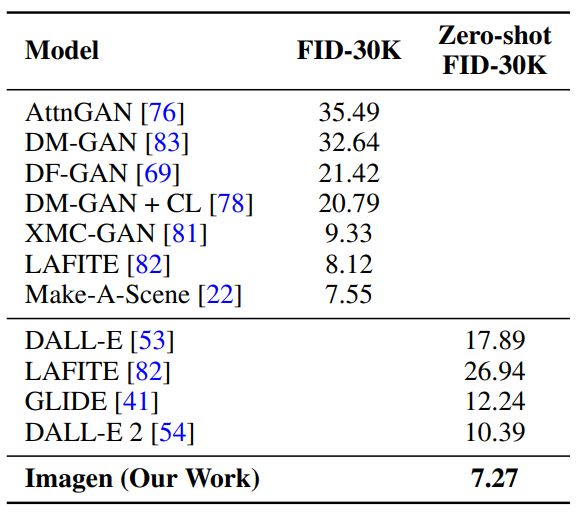
\includegraphics[width=0.6\linewidth]{images/imagen/imagen_coco_zeroshot.png}
        \caption{Although Imagen was not explicitly trained on MS-COCO dataset, it outperforms all other models on COCO FID score, achieving 7.27 FID.}
        \label{fig:imagen_coco_zeroshot}
    \end{subfigure}
    \begin{subfigure}{0.4\textwidth}
        \centering
        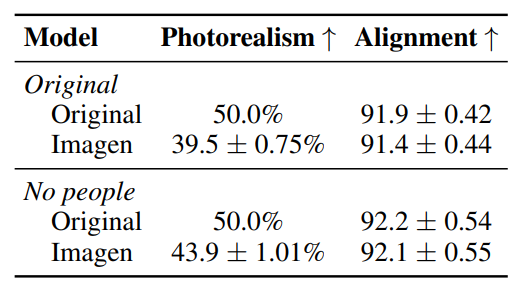
\includegraphics[width=0.6\linewidth]{images/imagen/imagen_coco_human_eval.png}
        \caption{Human evaluation on 256x256 COCO. Imagen splits to two categories: no filters, and human filters. Imagen struggles a little bit with photorealistic people.}
        \label{fig:imagen_coco_human_eval}
    \end{subfigure}
    \caption{Results of Imagen on COCO dataset \cite{imagen}.}
\end{figure}

\begin{figure}
    \centering
    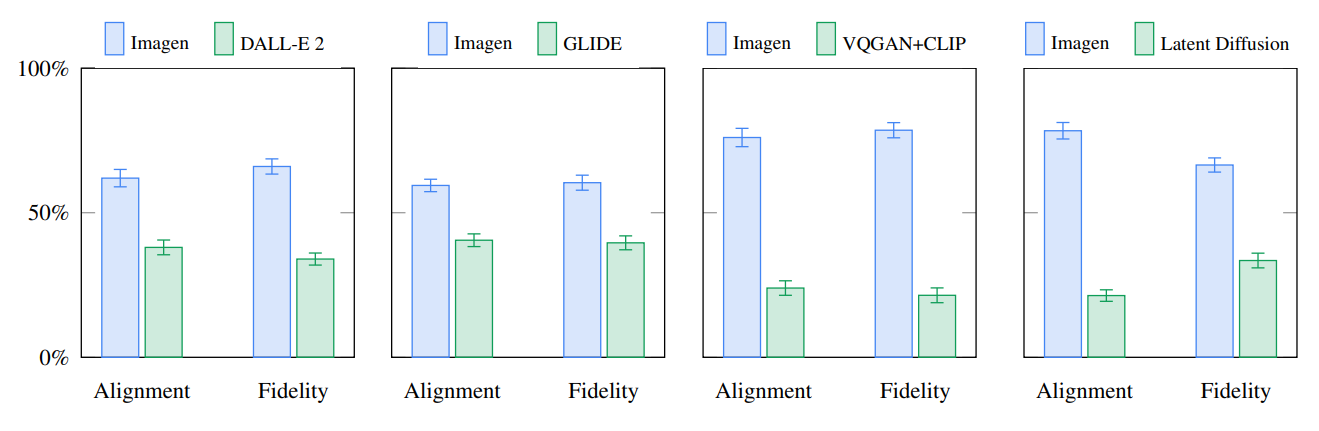
\includegraphics[width=0.6\textwidth]{images/imagen/alignment_fidelity_imagen_vs_models.png}
    \caption{Imagen beats all other models (DALL-E 2 \cite{dalle_2}, GLIDE \cite{glide}, VQGAN+CLIP \cite{vqgan_clip} and Latent Diffusion (Stable Diffusion) \cite{stable_diffusion} (section \ref{sec:stable_diffusion})) in terms of image-text alignment and image fidelity \cite{imagen}.}
    \label{fig:imagen_alignment_fidelity_vs_other_models}
\end{figure}

In figure \ref{fig:imagen_coco_zeroshot} we can see that although Imagen was not trained on the MS-COCO dataset, it still outperforms state-of-the-art models such as DALL-E 2 \cite{dalle_2} and achieves the best MS-COCO FID score of 7.27 in zero-shot setting.

In figure \ref{fig:imagen_coco_human_eval} we can see that Imagen achieves a respectable 43.9\% fool rate on $256\times 256$ COCO human faces, indicating limited ability of Imagen to generate photorealistic people.

In figure \ref{fig:imagen_alignment_fidelity_vs_other_models} we can see that Imagen outperforms all other state-of-the-art models in terms of image fidelity and text-image alignment.


% Video Generation
\section{Video Synthesis}
\label{sec:video_synthesis}

\begin{figure}
    \centering
    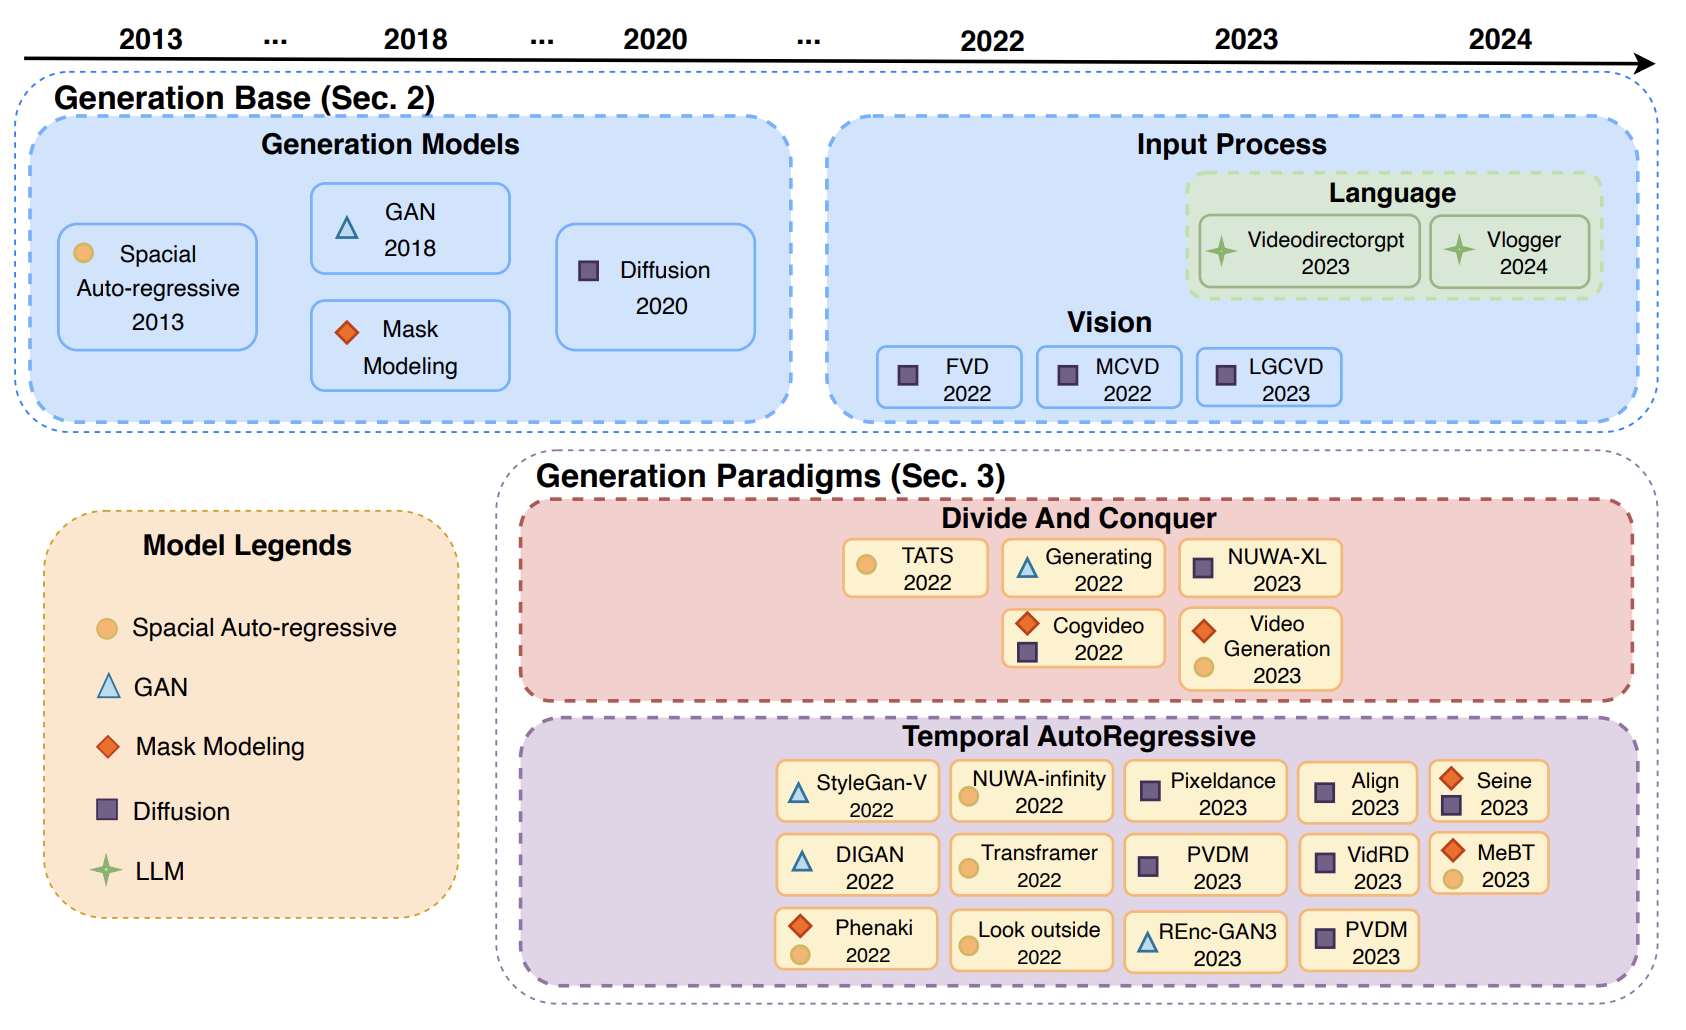
\includegraphics[width=0.7\textwidth]{images/video_synthesis/techniques.png}
    \caption{Overview of video synthesis techniques \cite{long_video_survey}.}
    \label{fig:video_synthesis_techniques}
\end{figure}

Video synthesis is a complex task. One can think of video generation as a sequence of image generation tasks. Formally, a video is a sequence of images (or frames) that are shown in fast fashion, usually 24 frames per second (at the minimum, to get smooth video). Therefor to create a video of 5 seconds, you'll need 120 frames or images at the minimum. Additional complexity is the addition of the \textbf{time dimension}, which is not present in image generation tasks. The video should be \textbf{coherent} in time, meaning that the frames should be related to each other and should follow a logical sequence. Objects should not appear out of nowhere, there should be \textbf{smooth transition of motion} and correct \textbf{spatial relationships} between objects. We also have to deal with limited hardware resources, since video generation is extremely computationally expensive.

% TODO: Add timeline of video synthesis models
% \begin{figure}
    \centering
    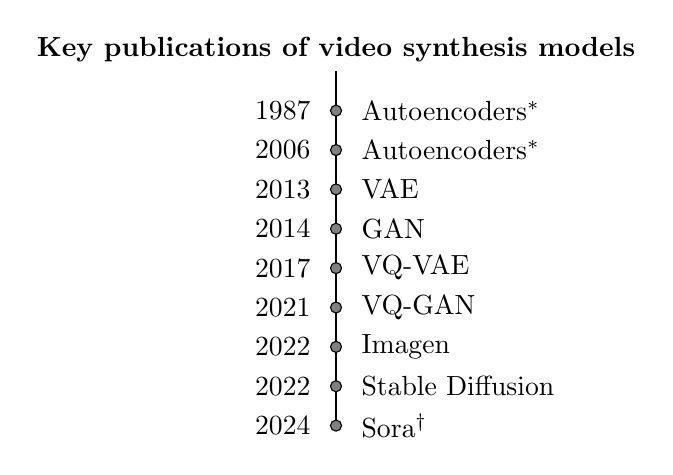
\begin{tikzpicture}
        \def\step{0.5} % step size for vertical spacing
        \def\numtimeline{9} % Number of events in the timeline

        % Define timeline line
        \draw[thick, color=black] (0,0) -- (0,-\numtimeline*\step);

        % Define timeline events with adjusted positions
        \foreach \i/\year/\text in 
        {
            1/1987/Autoencoders$^*$, 
            2/2006/Autoencoders$^*$, 
            3/2013/VAE, 
            4/2014/GAN, 
            5/2017/VQ-VAE,
            6/2021/VQ-GAN,
            7/2022/Imagen,
            8/2022/Stable Diffusion,
            9/2024/Sora$^\dag$
        } {
        \draw[fill=darkgray] (0,-\i*\step) circle (2pt);
        \node[anchor=east] at (-0.2,-\i*\step) {\year};
        \node[anchor=west] at (0.2,-\i*\step) {\text};
        }

        % Define timeline title
        \node[anchor=south] at (0,0) {\textbf{Key publications of video synthesis models}};
    \end{tikzpicture}
    \caption{Chronology of key video generation models publications.}
  \end{figure}

% There are a lot of techniques and models for video generation, and they can be divided into multiple categories:

% \begin{itemize}
%     \item \textbf{Frame prediction}: ...
%     \item \textbf{GAN based models}: such in the case of \cite{chu2020learning} the authors propose 
% \end{itemize}

Video synthesis can be based on four main models and methods:

\begin{enumerate}
    \item \textbf{Diffusion}: diffusion models for video generation extend the iterative refinement process used in image-based diffusion models, such as LDMs, to handle temporal dynamics required for videos. The key idea is to generate not just a sequence of independent images, but a continuous video where both the spatial content of each frame and the temporal coherence between frames are learned and generated simultaneously.
    \item \textbf{Spatial autoregressive}: spatial autoregressive models for video generation, as described in \cite{graves2013generating}, synthesize video by sequentially generating content in a patch-based fashion, where each patch in a frame is conditioned on previously generated patches. This method builds video frame-by-frame, ensuring spatial and temporal coherence across the entire sequence.
    \item \textbf{GAN}: similar to diffusion models, GANs can also be leveraged for video synthesis. 
    \item \textbf{Mask modeling}: mask modeling in video generation uses the technique of selectively masking parts of video frames during training to enhance the model's ability to learn spatial and temporal dependencies. By hiding portions of the video frames, the model is tasked with predicting and reconstructing the missing parts, forcing it to better understand the underlying structure and motion in the video.
\end{enumerate}

\begin{figure}
    \centering
    \includegraphics[width=1\textwidth]{images/video_synthesis/paradigms.png}
    \caption{Overview of video synthesis paradigms \cite{long_video_survey}. Divide and conquer is split into hierarchical architecture for keyframe generation and frame filling. Whereas temporal autoregressive paradigm the next frame prediction depends on the previous frame/frames.}
    \label{fig:video_synthesis_paradigms}
\end{figure}

In the realm of video synthesis there are two paradigms: \textbf{divide and conquer} and \textbf{temporal autoregressive}. An overview of the paradigms is shown in figure \ref{fig:video_synthesis_paradigms}.

\subsection*{Divide and Conquer}

Divide and conquer paradigm breaks the task of video synthesis into smaller, more manageable tasks. This approach can further by divided into 3 methods of approach:

\begin{enumerate}
    \item \textbf{Hierarchical architecture for frame generation}: in this approach, the process is split into \textbf{keyframe generation} and \textbf{frame filling}. Keyframes represent the critical moments of the video that establish the narrative, while the frame-filling models ensure smooth transitions between them. Global models focus on generating the main storyline through keyframes, and local models handle finer details, filling the gaps between the keyframes to maintain temporal consistency.
    \item \textbf{Multi-stage approach for video super-resolution}: \cite{brooks2022generating} suggested generating video by stages, first by creating low-resolution sequences with GAN and then applying super-resolution models to enhance them with StyleGAN3 \cite{stylegan3}.
    % TODO: Explain the combined process of mask modeling, I don't really understand. Maybe read the paper CogVideo?
    \item \textbf{Integrated keyframe and frame filling with mask modeling} simplifies long video generation by combining keyframe creation and frame filling into a unified process. Mask modeling hides specific parts of the video during training, keyframes and intermediate frames simultaneously, like done in CogVideo \cite{cogvideo}, which simplified mask modeling and combines these models into a single model.
\end{enumerate}

\subsection*{Temporal autoregressive}

Temporal autoregressive paradigm is an iterative approach where each frame is generated based on the previous one. The model is trained on sequences of video data, and the output from one timestep serves as the input for the next (the next frame is conditioned on the previous frame, which in theory ensures that the video is temporally coherent).

A significant amount of research has been conducted on temporal autoregressive models, leading to various improvement strategies and enhancements for this framework. Some of the most notable include:

\begin{itemize}
    \item \textbf{Latent space compression}: this method focuses on compressing videos to latent space to optimize computational needs. For example in \cite{zeng2024make} and \cite{gu2023reuse} they explored condensing video data into 3D latent. Compression aims to preserve essential features across dimensions to improve computational efficiency.
    \item \textbf{Incorporating temporal layers} to refine individual video clips. Advancements were made, such as integrating \textbf{temporal layers} (such as attention and convolutional layers) into diffusion models, like in VideoLDM \cite{video_ldm} and \cite{gu2023reuse}. These temporal layers help the model better understand the temporal dynamics of video data.
    \item \textbf{Dual-phase training \& reuse strategies}: dual-training is a training strategy where the model is first trained unconditionally, and then learn to conditionally generate video like in Projected Latent Video Diffusion Model (PVDM) \cite{pvdm}. Given the abundance of unlabeled video data on the web, it's easy to see why this process is attractive. Another method to boost the model's ability to replicate long video sequences is a \textbf{reuse strategy}, which iteratively adds and removes noise during training to simulate natural variability, like in \cite{gu2023reuse}.
\end{itemize}

\subsection*{Spatial autoregressive models}

Spatial autoregressive models are adept at processing tokenized sequence inputs (they include the transformer architecture) which enable the segmentation of video frames into patches. By integrating video data features with the autoregressive power of transformers, these models become more capable of capturing temporal dynamics. In this method, there are two main approaches:

\begin{itemize}
    \item \textbf{Frame tokenization}: like in NUWA-Infinity \cite{nuwa_infinity}, the researchers transform video frames into patches and combine them with spatial positional encodings for more efficient data handling. These autoregressive models, similar to LDMs, compress video data into latent space. Compression techniques like \textbf{Discrete Cosine Transform (DCT)} are used in Transframer \cite{transframer} and by using VQGAN, they convert the frames into latent tokens.
    \item \textbf{Scaling with attention mechanism}: architectural modifications were made by incorporating specialized blocks, such as attention mechanism blocks tailored for spatiotemporal data. For example, Transframer \cite{transframer} integrated temporal and spatial annotations (time-steps, camera viewport, etc.) through cross-attention.
\end{itemize}

\subsection*{Challenges in video synthesis}

Because video synthesis is still developing to this day and is a complex task, there are a lot of open questions to be asked:

\begin{itemize}
    \item How to generate long videos while maintaining high temporal cohesion?
    \item Would it be possible to generate videos in high resolution, with limited computational resources?
    \item How to train video generation models with abundant, unlabeled video data, such as YouTube? Are there any open datasets for video generation?
    \item How to generate videos from text, or other modalities? Is it possible to edit generated videos so it fits our artistic needs?
    \item What is considered a long video? Frame count (e.g., 512, 1024 frames)? Duration (e.g., 3, 5 minutes)?
    \item How we would trade off between resolution (high resolution) of generated video, duration (long), and spatial coherence (smooth motion and logical spatial relationships)? Can we achieve all three?
    \item How to deal with abrupt scene transitions? How to ensure smooth transitions between scenes?
    \item How to measure and evaluate temporal-spatial consistency between video generation models? How to tell if one clip is smoother and more coherent than the other?
\end{itemize}

In \cite{long_video_survey} they surveyed papers in the field of video generation and propose a definition for 'long' videos to exceed 10 seconds long, assuming frame rate of 10fps, or equivalently 100 frames.

\subsection{Evaluation metrics}

\begin{figure}
    \centering
    \includegraphics[width=1\textwidth]{images/video_synthesis/eval_metrics.png}
    \caption{Evaluation metrics in video generation \cite{long_video_survey}.}
    \label{fig:video_synthesis_eval_metrics}
\end{figure}

A common metric used for video generation models is the \textbf{Frechet Video Distance (FVD)} \cite{fvd}, which is an extension of Frechet Inception Distance (FID). FVD compares videos by both spatial and temporal features by using similar process as FID: using a pre-trained 3D ConvNet (i3D), where in FID they use InceptionV3. The i3D network was trained on Kinetics dataset (Kinetics Human Action Video Dataset), and the 3D convolutions capture local and global spatial patterns within the frames. In similar fashion as FID, they compare the distribution of features from generated videos and the FVD is calculated:

\begin{equation*}
    \text{FVD} = \left| \left| \mu_{\text{real}} - \mu_{\text{fake}} \right| \right|^2_2 + \text{Tr} \left( \Sigma_{\text{real}} + \Sigma_{\text{fake}} - 2 \left( \Sigma_{\text{real}} \Sigma_{\text{fake}} \right)^{1/2} \right)
\end{equation*}

The lower the FVD score, the better the video generation model is. A more comprehensive list of evaluation metrics is shown in figure \ref{fig:video_synthesis_eval_metrics}.





\subsection{Previous works}

In \textbf{VideoGAN} \cite{video_gan} (2016) the researchers proposed to use of the large amounts of unlabeled video in order to learn scene dynamics and motion, and capture temporal signals. They proposed a model with \textbf{spatio-temporal convolutional} architecture, and they extend GANs to video generation. They successfully created a video of 1 second long, the model explicitly models the foreground separately from the background, which allows the network to learn which objects are in motion, and which don't. The methodology in this work is autoregressive frame prediction.

In the case of \cite{video_generation_from_text}, where the goal is to generate video from text, they proposed a hybrid model that uses a conditional variational autoencoder (VAE) and a generative adversarial network (GAN). The VAE model will output a 'gist' which is a sketch (intermediate step), how the video will take form (colors, object layout) and the GAN model will apply a set of image filter kernels based on the input text to get an encoded text-gist feature vector and the framework predicts future frames.

\textbf{NUWA-Infinity} \cite{nuwa_infinity} by Microsoft AI (2022) is a text-to-video model that can generate videos in any arbitrary resolution and in any length. Because previous works that use the divide-and-conquer strategy (of using patches to generate image or video) doesn't consider the the dependencies between generated patches explicitly, they struggle to guarantee consistency of generated content. NUWA-Infinity uses the \textbf{autoregressive over autoregressive generation mechanism} that can generate variable-sized videos, in both duration and resolution. This mechanism uses a global patch-level autoregressive
model that considers the dependencies between patches, and a local token-level autoregressive model considers the dependencies between visual tokens within each patch.

\textbf{NUWA-XL} \cite{nuwa_xl} (2023, which is an upgraded version of NUWA-XL) is a diffusion model that uses 3D-UNet for keyframe generation (by global diffusion model) and keyframe filling (by local diffusion model). They also built a new dataset called 'FlintstonesHD' for benchmarking long video generation. Their method reduced inference time when generating 1024 frames from 7.55 minutes to 26 seconds (\textbf{a 94\% reduction in inference time}) on the same hardware.

In \cite{ge2022long} (2022 by Meta AI) they used a conditional (text or images) 3D VQ-GAN with hierarchical transformer architecture to generate long videos (1024 frames or more). They used standard benchmark datasets: UCF-101, Sky Time-lapse and Taichi-HD. They core insight is that using transformers is ideal for capturing long-range temporal dependence.

The OpenAI researchers introduced in a 2020 paper \textbf{Image-GPT (iGPT)} \cite{imagegpt}, in which they tried to explore autoregressive sequence transformer to predict pixels directly, without using CNN prior, only by using the attention mechanism. They pre-trained a transformer on ImageNet and showed that a transformer can learn spatial features (image representation learning). Instead of language tokens, the transformer predicts pixels. The biggest model, called iGPT-XL has 6.8 billion parameters. They also showed that when scaling transformers (more parameters, more pre-training) the architecture quickly closes the gap on contrastive learning of other models that specifically design to this task.

\textbf{VideoGPT} \cite{videogpt} (2021), which we will take a closer look in section \ref{sec:videogpt}, uses VQ-VAE to encode video frames into discrete latent representations by using 3D convolutions and self-attention. It also uses a transformer based on the work of Image-GPT to generate video frames from the latent representations. VideoGPT uses the same prior networks as Image-GPT \cite{imagegpt}.

\textbf{Imagen-Video} \cite{imagen_video} (2022) by Google is a text conditional video generation system based on a cascade of video diffusion models (similar to Imagen (section \ref{sec:imagen})). Instead of 2D super-resolution models as we seen in Imagen, they are spatial and temporal video super-resolution models. Similar to Imagen it also uses frozen T5-XXL \cite{t5_model} text encoder (for text embeddings), it consists of 7 sub-models (1 base model, 3 spatial super-resolution models [SSRs], and 3 temporal super-resolution models [TSRs]) to generate videos of high resolution (1280x768) of 24 frames per second for 5.4 seconds. The diffusion model is 11.6 billion parameters (not including the text encoder). The TSR models increase temporal resolution, whereas SSR increase spatial resolution. The researchers build upon the previous work of \textbf{Video U-Net} architecture \cite{video_diffusion_models}.

\begin{figure}
    \centering
    \includegraphics[width=1\textwidth]{images/video_synthesis/imagen_video.png}
    \caption{Imagen-Video video samples examples.}
\end{figure}

In \cite{video_diffusion_models} (2022) by Google proposed a diffusion model for video generation, which is an extension of the standard image diffusion architecture, and can be trained by both images and videos. They proposed to use a \textbf{3D U-Net architecture} in a standard diffusion model to extend to the video domain. They changed the 2D convolution to space-only 3D convolution (if $k$ is the kernel size, then we convert $k\times k$ convolution to $1\times k\times k$), and after each spatial attention block they insert temporal attention block that performs a temporal attention on the first axis. They also use relative position embeddings, similar to positional or time embeddings, so the network can distinguish ordering of video frames.

\textbf{To summarize}, there is a common consensus among the researchers in the previous works. They agree that in order to generate high-cohesion long videos, we need to model long-range temporal dependence in videos with many more frames. Not only that, but also that base models GANs are difficult to optimize for video generation tasks because of the adversarial loss, unlike the likelihood loss found in every other base model (VAE, diffusion, transformers). And finally, they agree that \textit{"the video domain has not yet witnessed its 'AlexNet moment'"} [quote from \cite{tran2018closer}] (AlexNet \cite{alexnet} was a major breakthrough in 2012 for image classification task which led to the development of imaging domain in deep learning). 






\subsection{Spatiotemporal feature learning}

\begin{figure}
    \centering
    \includegraphics[width=1\textwidth]{images/video_synthesis/conv.png}
    \caption{2D and 3D convolution operations. (a) Applying 2D convolution on image results in an image. (b) Applying 2D convolution on video (multiple frames) also results in an image. (c) Applying 3D convolution on video results in another volume (channel), preserving temporal information. Figure from the 2014 paper \cite{tran2015learning}.}
\end{figure}

A 2014 paper \cite{tran2015learning} by Facebook AI suggested using 3D-ConvNets (3D convolution networks) for video data spatiotemporal feature learning. The dataset that they used are UCF101, Sports-1M, and because Sports-1M has 100x times the amount of video clips compared to UCF101. For each video clip, they extracted five 2-second clips as the train-test split and resized the frames to 128x171, and flipped the frames horizontally with 50\% probability.

Compared to 2D ConvNet, 3D ConvNet has the ability to model temporal information better owing to 3D convolution and 3D pooling operations. The researchers found that 3x3x3 kernel size is the best option for 3D ConvNets. After every 3D convolution layer they apply 3D max-pooling.

\begin{figure}
    \centering
    \includegraphics[width=1\textwidth]{images/video_synthesis/c3d_feature_maps.png}
    \caption{Feature maps of the first 3D convolution layer of the C3D model \cite{tran2015learning}. The first two rows of the feature maps shows the detection of moving edges and blobs, while the last row shows edge orientation changes and color changes.}
    \label{fig:c3d_feature_maps}
\end{figure}

Figure \ref{fig:c3d_feature_maps} shows the feature maps of the first 3D convolution layer of the C3D model. The 3D convolution helps to capture motion between frames.

In a 2018 paper \cite{tran2018closer} that reviews spatiotemporal convolution (also by Facebook AI), they observed that 2D CNNs applied on individual frames of video remain solid performers in action recognition (the classification of action [like cooking, running, dancing] in image/video). By using residual connections, and by factorizing the 3D convolutional filters into separate spatial and temporal components results in the creation of a new spatiotemporal convolution block called \texttt{R(2+1)D}. The \texttt{R(2+1)D} block is a 2D residual block followed by a 1D temporal convolution. This separation allows the model to represent more complex non-linear functions, and is more easily optimized.


\subsection{Optimizations \& Context Reduction}

\textbf{Color reduction}: In \cite{imagegpt} they proposed context reduction: first by downsizing the resolution of the training videos to lower resolution, and more importantly, they created their own 9-bit color palette by K-mean clustering (k=512). That means, each pixel is represented by 9 bits, instead of 256x256x256 (which require 8+8+8=24 bits). This color reduction yields a sequence length three times shorter than the standard (R, G, B) palette.



% Previous works
\section{VideoGPT}

\begin{figure}
    \centering
    \includegraphics[width=0.7\textwidth]{images/video_synthesis/videogpt_architecture.png}
    \caption{VideoGPT architecture.}
\end{figure}

\begin{figure}
    \centering
    \includegraphics[width=0.5\textwidth]{images/video_synthesis/videogpt_res_atten_block.png}
    \caption{Residual attention block as described in VideoGPT.}
    \label{fig:videogpt_res_atten_block}
\end{figure}

% TODO: Explain 3D convolutions
VideoGPT \cite{videogpt} uses likelihood based model VQ-VAE and GPT-like transformer model. The encoder of VQ-VAE first downsamples video into discrete latent space using 3D convolutions, and the decoder then reconstructs the video from these latent codes (by using a codebook - see VQ-VAE section \ref{sec:vqvae}). The generated latents are decoded to the original video resolution as the training dataset.

The researchers take inspiration from image and video codecs: JPEG and MPEG for image and video compression. They contain the same spatio-temporal data as the uncompressed video, yet take less resources (by not working in the pixel space).

Reminder that the loss function of VQ-VAE is defined:

\begin{equation*}
    \mathcal{L} = \underbrace{\left| \left| x - D(e) \right| \right|^2_2}_{\mathcal{L}_\text{recon}} + \underbrace{\left| \left| \text{sg}\left[ E(x) \right] - e \right| \right|^2_2}_{\mathcal{L}_\text{codebook}} + \underbrace{\beta \left| \left| \text{sg}[e] - E(x) \right| \right|^2_2}_{\mathcal{L}_\text{commit}}
\end{equation*}

where $\text{sg}$ refers to stop-gradient, $\mathcal{L}_\text{recon}$ is the reconstruction loss (mean squared error), $\mathcal{L}_\text{codebook}$ is the codebook loss (quantization loss), and $\mathcal{L}_\text{commit}$ is the commitment loss. The decoder optimizes the reconstruction loss only, the encoder optimizes the commitment loss only, and the codebook embeddings are optimized in the codebook loss (depending on the stop-gradient). See section \ref{sec:vqvae} for more details.

The researchers used EMA update \cite{vqvae} for the codebook loss which is a (exponential) moving average of the codebook embeddings. In short, it makes the VQ-VAE faster to train and faster convergence speed.

As described in section \ref{sec:vqgan}, GPT is autoregressive transformer model. The autoregressive nature can be described as $p(x) = \prod_{i=1}^{d} p(x_i | x_{\leq i})$ through masked self-attention.






\subsection{Architecture}

They train the VQ-VAE on video data to learn the codebook. The encoder and decoder consists of 3D convolutions (appendix \ref{appendix:blocks_3dconv}) followed by attention residual blocks (figure \ref{fig:videogpt_res_atten_block}). Axial attention block is described in appendix \ref{appendix:blocks_axial_attention}.
% \section{Sora}

% TODO: Add more
Sora by OpenAI is a video synthesis model, if not one of the best video synthesis models to date. It was introduced in a 2023 paper \cite{sora}. The model is based on the principles of Stable Diffusion, Video-LDM and DiT. They leverage the scalability of the transformer architecture in DiT and use their already pre-trained GPT-4o model as the backbone (\cite{sun2024sora} section 3.1.2). The innovation in Sora is the use of diffusion, working in latent space, replacing U-Net with transformers, and the use of both adaptive layer norm and cross-attention for text conditioning.



% Main works
\section{Video-LDM}
\label{sec:videoldm}

\begin{figure}
    \centering
    \includegraphics[width=0.7\textwidth]{images/video_ldm/stack.png}
    \caption{Video-LDM stack. (1) The network generates keyframes latents. (2) Between each two keyframes, the network learns to interpolate between (keyframe filling). (3) Between each two frames in the frame filling, they act as new keyframes and the process repeats once more (they use the same interpolation model, same parameters). (4) The latents are decoded to pixel space. (5) Super-resolution model is applied (optionally) to upsample the video resolution.}
\end{figure}

Video-LDM by NVIDIA (2023) \cite{video_ldm} is a text-to-video synthesis model that uses LDM (Latent Diffusion Model, more commonly called Stable Diffusion, section \ref{sec:stable_diffusion}). The main idea of Video-LDM is to first train the model as image generator; and then transform it into a video generator. Its also possible to use pre-trained LDM and then fine-tune it and convert it to a video generator. The model can output in a resolution of up to 1280x2048, which is considered very high resolution in the field of video synthesis.

First, the model is pre-trained with image only datasets; then, temporal layers are added to the LDM that learn to align images in temporally consistent manner; then the model is trained on video datasets and only the temporal layers are learned (the other layers are frozen).

The idea to insert temporal layers into pre-trained generators has been explored by the GAN-based methods MoCoGAN-HD \cite{mocogan_hd} and StyleVideoGAN \cite{style_video_gan} before, but at much smaller scale.

\begin{figure}
    \centering
    \includegraphics[width=0.8\textwidth]{images/video_ldm/ddpm_sde.png}
    \caption{Generative modeling through stochastic differential equations (SDE) \cite{song2020score}. It shows how data distribution $p(x)$ slowly transforms to prior distribution $p_T(x)$ through forward SDE (we add noise) and then reversed back to generate data with reverse SDE. The colored lines show the SDE paths which represent sample trajectories through the diffusion process. The lines converge at the prior, the noise causes data samples to become progressively less structured, transitioning from a well-defined data distribution to a more chaotic noise-like distribution. The left side shows the probability of the data, the middle shows the probability of the prior (Gaussian distribution), and the right shows we are back to the original data distribution.}
\end{figure}

\begin{figure}
    \centering
    \includegraphics[width=0.8\textwidth]{images/video_ldm/image_to_video_tuning.png}
    \caption{Transforming image LDM (left) to video LDM (right) \cite{video_ldm}. \textit{Per-batch element denoising}: the stochastic denoising process of diffusion. \textit{Batch/Video Frame Axis}: on the left each image generated is not correlated to other images in the batch; on the right each generated image is correlated to the previous image, the model learns to align them and generate temporally consistent video. \textit{Batch/Video Frame Axis}: the red arrows and line shows how one image transitions to the next image, creating the video.}
    \label{fig:video_ldm_image_to_video_tuning}
\end{figure}





\subsection*{Mathematical notations}

The LDMs autoencoder compresses the high-dimensional input data $x \in \mathbb{R}^{T \times 3 \times \hat{H} \times \hat{W}}$ where $x \sim p_{\text{data}}$ is a sequence of $T$ RGB frames with height $\hat{H}$ and width $\hat{W}$ to lower-dimensional latent space $z = \mathcal{E} (x) \in \mathbb{R}^{T \times C \times H \times W}$ (where $C$ is the number of latent channels, and $H, W$ are the spatial latent dimensions) in order to improve computational needs. The model then learns to reconstruct $x$ via decoder $\mathcal{D}$: $\hat{x} = \mathcal{D} (\mathcal{E} (x)) \sim x$.

Let us denote the layers of the LDM (without temporal layers) as spatial layers $l^i_{\theta}$ where $\theta$ are the model's parameters, and $i$ is the layer index. We then denote the addition of temporal layers as $l^i_{\phi}$ to learn to align individual frames in a temporally consistent manner. We denote $f_{\theta, \phi}$ as the full model (with spatial and temporal layers).






\subsection{Architecture}

\begin{figure}
    \centering
    \includegraphics[width=0.6\textwidth]{images/video_ldm/enc_dec_denoise_process.png}
    \caption{Top: frozen encoder compresses video frames into 3D latents and the decoder learns to reconstruct image from the latent (like in autoencoders). The patch-based discriminator $\mathcal{H}$ is used to increase photorealism, the adversarial objective is added to the autoencoder reconstruction score like in PatchGAN (\cite{isola2017image} which tries to classify if $N \times N$ patch is real or fake). \textit{Bottom}: generative denoising process, each embedding corresponds to different image generation in the decoder $\mathcal{D}$.}
\end{figure}

\begin{figure}
    \centering
    \includegraphics[width=0.6\textwidth]{images/video_ldm/temporal_layers.png}
    \caption{\textit{Left:} The researchers turn pre-trained LDM into video generator by adding temporal layers $l_\phi$ that learn to align images in a temporally consistent manner. The spatial layers $l_\theta$ are frozen and only the temporal layers are learned. \textit{Right:} closer look into spatial, temporal layers of the left side (a single U-Net block). In order to deal with the addition of the temporal dimension, they rearranged the batch dimension in LDM to be mixed with the temporal dimension for the next layer: $(b\ t)\ c\ h\ w \rightarrow b\ t\ c\ h\ w$. The $c_S$ represents a context vector used for conditioning the model.}
    \label{fig:video_ldm_spatial_temporal_mixing_layers}
\end{figure}

The architecture of Video-LDM is similar to Stable Diffusion with the exception of added temporal layers, and the addition of autoencoder for latent encoding/decoding and the discriminator which helps photorealism in the decoder network.

The input of the spatial layers $l_\theta^i$ is of the dimension $b\ c\ h\ w$ whereas the input dimension of temporal layers is of the dimension $b\ t\ c\ h\ w$. This notation is called \texttt{Einops} and is discussed in the Einops paper \cite{einops}. The spatial layers interpret the video as a batch of images by shifting the temporal axis into the batch dimension (the spatial layers treat all $B \cdot T$ encoded video frames in the batch dimension $b$). 

For the 3D convolution (temporal layer), they reshape the input back to video dimensions (they process entire videos in new temporal dimension $t$): 

\[ \underbrace{(b\ t)\ c\ h\ w}_{\text{Output of spatial layer}} \rightarrow \underbrace{b\ c\ t\ h\ w}_{\text{Input to the next Conv3D layer}} \]

After the temporal layers they reshape the input back to fit into the spatial layers like so:

\[ \underbrace{b\ c\ t\ h\ w}_{\text{Output of Conv3D layer}} \rightarrow \underbrace{(b\ t)\ c\ h\ w}_{\text{Input to the next spatial layer}} \]

As for the temporal attention layer (temporal layer), they reshaped the input back to work on the temporal dimension, instead of spatial:

\[ \underbrace{(b\ t)\ c\ h\ w}_{\text{Output of spatial layer}} \rightarrow \underbrace{(b\ h\ w) \ t\ c}_{\text{Input to the next temporal attention layer}} \]

\[ \underbrace{(b\ h\ w) \ t\ c}_{\text{Output of temporal attention layer}} \rightarrow \underbrace{(b\ t)\ c\ h\ w}_{\text{Input to the next spatial layer}} \]

To help us visualize how this reshaping operation works, lets think about 3D cube. The width and height are the spatial width, height of images, and the depth is the temporal dimension (frames of video). Now, lets drop the channels, because its another dimension to think about (each image has 3 channels). Then we can think about temporal operations as a 2D plane slice on the temporal axis. And spatial layers: we can think of them as they work from the width, height dimensions. In both cases, we work in batches, but if we think about batch size of 1 then its easier to understand.

\begin{figure}
    \centering

    \begin{subfigure}{0.3\textwidth}
        \centering
        \scalebox{0.6}{
            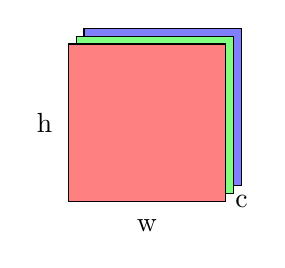
\begin{tikzpicture}
    % Blue channel slice
    \draw[fill=blue!50] (0, 0) rectangle (2, 2);

    % Green channel slice
    \draw[fill=green!50] (-0.1, -0.1) rectangle (1.9, 1.9);
    
    % Red channel slice
    \draw[fill=red!50] (-0.2, -0.2) rectangle (1.8, 1.8);

    \node at (0.8, -0.5) {w};
    \node at (-0.5, 0.8) {h};
    \node at (2, -0.2) {c};
    
\end{tikzpicture}

        }
        \caption{A single frame. The $c\ h\ w$ dimensions.}
    \end{subfigure}

    \begin{subfigure}{0.3\textwidth}
        \centering
        \scalebox{0.6}{
            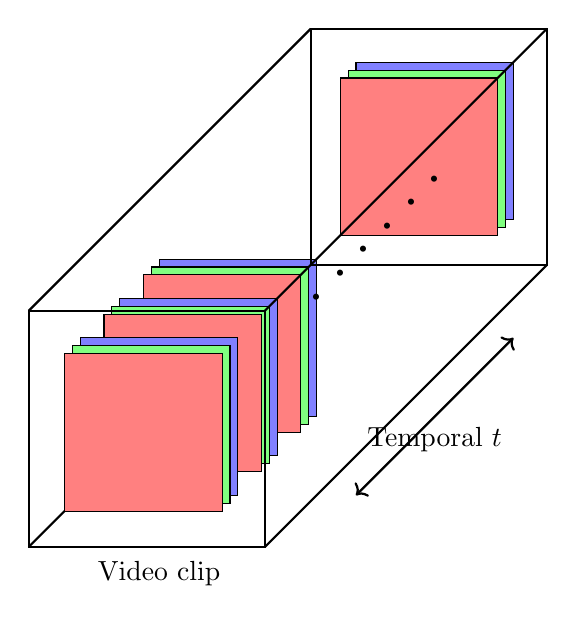
\begin{tikzpicture}
    % 3D Cube - we want to draw some of the cube edges below the frames
    % variables
    \def\cubeWidth{3}
    \def\cubeHeight{3}
    % \def\cubeDepth{8}

    % Cube points
    \coordinate (A) at (0, 0, -5);
    \coordinate (B) at (\cubeWidth, 0, -5);
    \coordinate (C) at (\cubeWidth, \cubeHeight, -5);
    \coordinate (D) at (0, \cubeHeight, -5);
    \coordinate (E) at (-0.5, -0.5, 3);
    \coordinate (F) at (\cubeWidth - 0.5, -0.5, 3);
    \coordinate (G) at (\cubeWidth - 0.5, \cubeHeight - 0.5, 3);
    \coordinate (H) at (-0.5, \cubeHeight - 0.5, 3);

    % Draw cube edges that are below the frames
    \draw[thick] (A) -- (E);

    \def\width{2}
    \def\height{2}
    \def\shift{0.1} % Shift for the green and red channels

    \def\xshift{-0.5}  % Shift in the x direction for duplication
    \def\yshift{-0.5}  % Shift in the y direction for duplication
    \def\lastrectxshift{\xshift * -5} % Last image should be shifted more because of three dots
    \def\lastrectyshift{\yshift * -5} % Last image should be shifted more because of three dots
    \def\dotstartx{2}  % Starting x position for the dots
    \def\dotstarty{1.5}  % Starting y position for the dots
    \def\dotshift{0.3}  % Shift for the dots


    % First rectangle
    \draw[fill=blue!50] (0, 0) rectangle (\width, \height);
    \draw[fill=green!50] (-\shift, -\shift) rectangle (\width-\shift, \height-\shift);
    \draw[fill=red!50] (-2*\shift, -2*\shift) rectangle (\width-2*\shift, \height-2*\shift);

    % Second rectangle
    \draw[fill=blue!50] (\xshift, \yshift) rectangle (\xshift+\width, \yshift+\height);
    \draw[fill=green!50] (\xshift-\shift, \yshift-\shift) rectangle (\xshift+\width-\shift, \yshift+\height-\shift);
    \draw[fill=red!50] (\xshift-2*\shift, \yshift-2*\shift) rectangle (\xshift+\width-2*\shift, \yshift+\height-2*\shift);

    % Third rectangle
    \draw[fill=blue!50] (2*\xshift, 2*\yshift) rectangle (2*\xshift+\width, 2*\yshift+\height);
    \draw[fill=green!50] (2*\xshift-\shift, 2*\yshift-\shift) rectangle (2*\xshift+\width-\shift, 2*\yshift+\height-\shift);
    \draw[fill=red!50] (2*\xshift-2*\shift, 2*\yshift-2*\shift) rectangle (2*\xshift+\width-2*\shift, 2*\yshift+\height-2*\shift);

    % Fourth rectangle
    \draw[fill=blue!50] (\lastrectxshift, \lastrectyshift) rectangle (\lastrectxshift+\width, \lastrectyshift+\height);
    \draw[fill=green!50] (\lastrectxshift-\shift, \lastrectyshift-\shift) rectangle (\lastrectxshift+\width-\shift, \lastrectyshift+\height-\shift);
    \draw[fill=red!50] (\lastrectxshift-2*\shift, \lastrectyshift-2*\shift) rectangle (\lastrectxshift+\width-2*\shift, \lastrectyshift+\height-2*\shift);


    % Dots
    \node at (\dotstartx, \dotstarty) {\huge$\cdot$};
    \node at (\dotstartx + \dotshift, \dotstarty + \dotshift) {\huge$\cdot$};
    \node at (\dotstartx + \dotshift*2, \dotstarty + 2*\dotshift) {\huge$\cdot$};
    \node at (\dotstartx + \dotshift*3, \dotstarty + 3*\dotshift) {\huge$\cdot$};
    \node at (\dotstartx + \dotshift*4, \dotstarty + 4*\dotshift) {\huge$\cdot$};
    \node at (\dotstartx + \dotshift*5, \dotstarty + 5*\dotshift) {\huge$\cdot$};

    % Arrow
    \draw[<->, thick] (2.5, -1) -- (4.5, 1) node[midway, below] {Temporal $t$};







    % Draw the rest of the cube
    \draw[thick] (A) -- (B) -- (C) -- (D) -- cycle;
    \draw[thick] (E) -- (F) -- (G) -- (H) -- cycle;
    \draw[thick] (B) -- (F);
    \draw[thick] (C) -- (G);
    \draw[thick] (D) -- (H);

    % Draw clip text
    \node at (0, -2) {Video clip};

    

\end{tikzpicture}

        }
        \caption{Multiple frames. The $t\ c\ h\ w$ dimensions.}
    \end{subfigure}

    \begin{subfigure}{0.7\textwidth}
        \centering
        \scalebox{0.6}{
            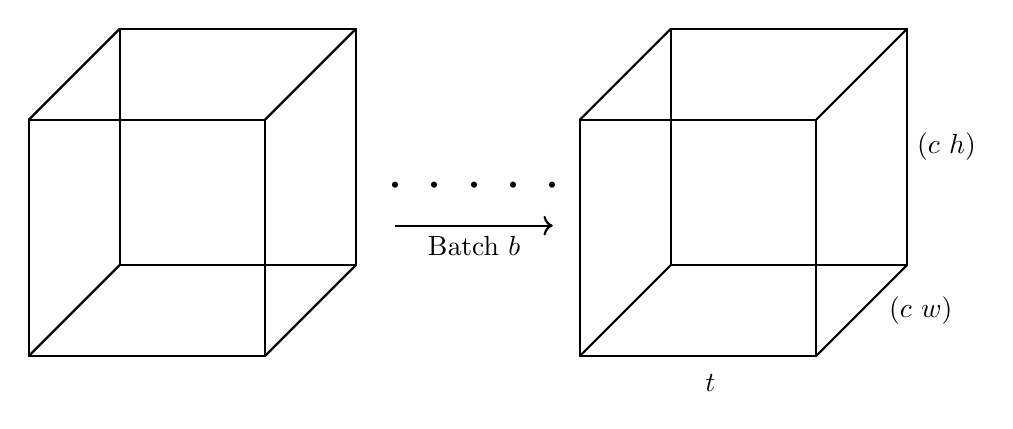
\begin{tikzpicture}
    % First cube
        % variables
        \def\cubeWidth{3}
        \def\cubeHeight{3}
        \def\cubeDepth{3}
    
        % Cube points
        \coordinate (A) at (0, 0, 0);
        \coordinate (B) at (\cubeWidth, 0, 0);
        \coordinate (C) at (\cubeWidth, \cubeHeight, 0);
        \coordinate (D) at (0, \cubeHeight, 0);
        \coordinate (E) at (0, 0, \cubeDepth);
        \coordinate (F) at (\cubeWidth, 0, \cubeDepth);
        \coordinate (G) at (\cubeWidth, \cubeHeight, \cubeDepth);
        \coordinate (H) at (0, \cubeHeight, \cubeDepth);
    
        % Draw cube
        \draw[thick] (A) -- (B) -- (C) -- (D) -- cycle;
        \draw[thick] (E) -- (F) -- (G) -- (H) -- cycle;
        \draw[thick] (A) -- (E);
        \draw[thick] (B) -- (F);
        \draw[thick] (C) -- (G);
        \draw[thick] (D) -- (H);
    
        % Axes
        \node at (0.5, -1.5, 0) {$t$};
        \node at (\cubeWidth + 0.5, \cubeHeight/2, 0) {$(c\ h)$};
        \node at (\cubeWidth + 0.75, 0, \cubeDepth/2) {$(c\ w)$};

    % Second cube
        % variables
        \def\cubeShiftX{-7}
        \def\cubeShiftY{0}
    
        % Cube points (shifted)
        \coordinate (A') at (\cubeShiftX, \cubeShiftY, 0);
        \coordinate (B') at (\cubeShiftX + \cubeWidth, \cubeShiftY, 0);
        \coordinate (C') at (\cubeShiftX + \cubeWidth, \cubeShiftY + \cubeHeight, 0);
        \coordinate (D') at (\cubeShiftX, \cubeShiftY + \cubeHeight, 0);
        \coordinate (E') at (\cubeShiftX, \cubeShiftY, \cubeDepth);
        \coordinate (F') at (\cubeShiftX + \cubeWidth, \cubeShiftY, \cubeDepth);
        \coordinate (G') at (\cubeShiftX + \cubeWidth, \cubeShiftY + \cubeHeight, \cubeDepth);
        \coordinate (H') at (\cubeShiftX, \cubeShiftY + \cubeHeight, \cubeDepth);
    
        % Draw the second cube
        \draw[thick] (A') -- (B') -- (C') -- (D') -- cycle;
        \draw[thick] (E') -- (F') -- (G') -- (H') -- cycle;
        \draw[thick] (A') -- (E');
        \draw[thick] (B') -- (F');
        \draw[thick] (C') -- (G');
        \draw[thick] (D') -- (H');

    % Three dots
        % variables
        \def\dotStartX{-3.5}
        \def\dotStartY{1}
        \def\dotShiftX{0.5}
        \def\dotShiftY{0}
    
        % dots
        \node at (\dotStartX, \dotStartY) {\huge$\cdot$};
        \node at (\dotStartX + \dotShiftX, \dotStartY + \dotShiftY) {\huge$\cdot$};
        \node at (\dotStartX + \dotShiftX * 2, \dotStartY + \dotShiftY * 2) {\huge$\cdot$};
        \node at (\dotStartX + \dotShiftX * 3, \dotStartY + \dotShiftY * 3) {\huge$\cdot$};
        \node at (\dotStartX + \dotShiftX * 4, \dotStartY + \dotShiftY * 4) {\huge$\cdot$};


    % Arrow
    \draw[->, thick] (-3.5, 0.5) -- (-1.5, 0.5) node[midway, below] {Batch $b$};
\end{tikzpicture}
        }
        \caption{All of the $b\ t\ c\ h\ w$ dimensions. }
    \end{subfigure}

    \begin{subfigure}{0.7\textwidth}
        \centering
        \scalebox{0.6}{
            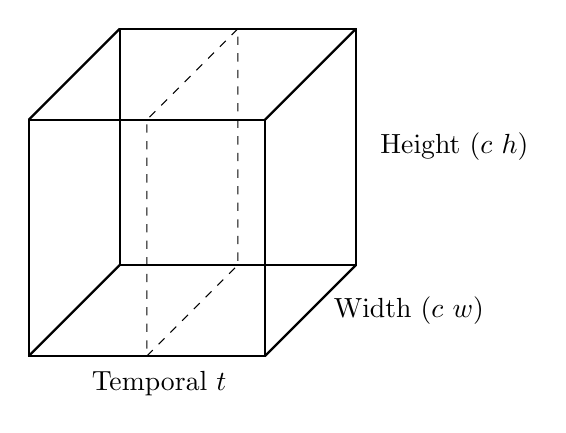
\begin{tikzpicture}
    % variables
    \def\cubeWidth{3}
    \def\cubeHeight{3}
    \def\cubeDepth{3}
    \def\slicePosition{1.5}

    % Cube points
    \coordinate (A) at (0, 0, 0);
    \coordinate (B) at (\cubeWidth, 0, 0);
    \coordinate (C) at (\cubeWidth, \cubeHeight, 0);
    \coordinate (D) at (0, \cubeHeight, 0);
    \coordinate (E) at (0, 0, \cubeDepth);
    \coordinate (F) at (\cubeWidth, 0, \cubeDepth);
    \coordinate (G) at (\cubeWidth, \cubeHeight, \cubeDepth);
    \coordinate (H) at (0, \cubeHeight, \cubeDepth);

    % Draw cube
    \draw[thick] (A) -- (B) -- (C) -- (D) -- cycle;
    \draw[thick] (E) -- (F) -- (G) -- (H) -- cycle;
    \draw[thick] (A) -- (E);
    \draw[thick] (B) -- (F);
    \draw[thick] (C) -- (G);
    \draw[thick] (D) -- (H);

    % Draw slice in middle
    \draw[dashed] (\slicePosition, 0, \cubeDepth) -- (\slicePosition, 0, 0) -- (\slicePosition, \cubeHeight, 0) -- (\slicePosition, \cubeHeight, \cubeDepth) -- cycle;

    % Axes
    \node at (0.5, -1.5, 0) {Temporal $t$}; 
    \node at (\cubeWidth + 1.25, \cubeHeight/2, 0) {Height $(c\ h)$};
    \node at (\cubeWidth + 1.25, 0, \cubeDepth/2) {Width $(c\ w)$};
\end{tikzpicture}
        }
        \caption{The $t\ c\ h\ w$ dimensions. The slice in the middle shows a single frame of dimension $(b\ t\ c)\ h\ w$, all of the first three dimensions collapse into the channel dimension.}
    \end{subfigure}

    \caption{Representation of video dimensions ($b\ t\ c\ h\ w$ which corresponds to batch, temporal, channel, height, width dimensions in video) to better understand input reshaping in spatial and temporal layers of Video-LDM.}
\end{figure}





\textbf{Mixing factor:} after each temporal layer, the output $z'$ is combined with the output of previous spatial layer output $z$ to form a mixing: 

\[ \underbrace{\alpha_\phi^i z_{i} + (1 - \alpha_\phi^i) z_{i}'}_{\text{Mixing factor}} \] 

where $\alpha_\phi^i \in [0, 1]$ and is a learnable parameter. If we set $\alpha = 1$ for each layer skip the temporal score and we retain the native image generation capability. This mixing operation is similar to Classifier-free Guidance (CFG) (mixing between conditional score and unconditional score).

\textbf{Temporal mixing layers:} two types of temporal mixing layers in use (see figure \ref{fig:video_ldm_spatial_temporal_mixing_layers}) are the \textit{temporal attention} and \textit{Conv3D} layer. The temporal attention layer is similar to the spatial attention layer, but it operates on the temporal dimension.

\textbf{Noise scheduler:} Video-LDM uses the same noise scheduler as the underlying image model. In table 6 of the paper, it shows that in all of their models, they use linear noise scheduler.

\textbf{Training objective:} the training objective is likelihood based, and only the temporal layers are trained. The objective is like the LDM objective (score matching objective of predicted noise in U-Net, basically mean squared error (MSE)):

\[ \arg \min_\phi \mathbb{E}_{x \sim p_{\text{data}}, \tau \sim p_{\tau}, \epsilon \sim \mathcal{N} (0, I)} \left[ \left| \left| y - f_{\theta,\phi} (z_{\tau} ; c, \tau) \right| \right|^2_2 \right] \]

where $\tau$ is the diffusion time step, $y$ is the target noise vector. The target is to minimize the difference between predicted noise and ground truth $y$ over all video frames (with mean squared error).

\textbf{Adding temporal layers to the autoencoder's decoder:} the researchers add temporal layers to the decoder of the autoencoder which they found this step to be critical for achieving good results. The reason is that the autoencoder is trained on images and flickering artifacts are present in the generated videos (because training on images doesn't teach the model temporal dynamics). So the researchers fine-tune the decoder on video data with a \textbf{patch-wise temporal discriminator built from 3D convolutions}. The encoder, however, remains unchanged.

\textbf{Patch-wise temporal discriminator:} The patch-wise temporal discriminator $\mathcal{H}$, which is built from 3D convolutions, is used to fine-tune the autoencoder (decoder only, encoder is frozen) on video data. It takes in video as input, and returns "real" or "fake" prediction on patches of the video clip.


\begin{figure}
    \centering
    \scalebox{0.5}{
        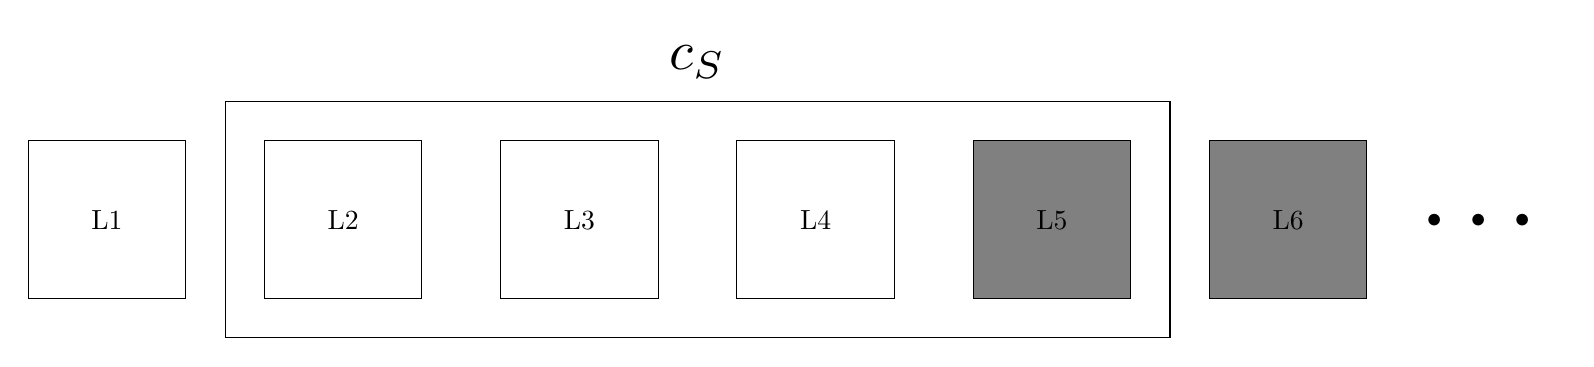
\begin{tikzpicture}
    \draw[fill=white!50] (0, 0) rectangle (2, 2);
    \node[anchor=center] at (1, 1) {L1};

    \draw[fill=white!50] (3, 0) rectangle (5, 2);
    \node[anchor=center] at (4, 1) {L2};

    \draw[fill=white!50] (6, 0) rectangle (8, 2);
    \node[anchor=center] at (7, 1) {L3};

    \draw[fill=white!50] (9, 0) rectangle (11, 2);
    \node[anchor=center] at (10, 1) {L4};

    \draw[fill=black!50] (12, 0) rectangle (14, 2);
    \node[anchor=center] at (13, 1) {L5};

    \draw[fill=black!50] (15, 0) rectangle (17, 2);
    \node[anchor=center] at (16, 1) {L6};

    % c_S
    \node[anchor=center, scale=2] at (8.5,3) {$c_S$};

    % Context guidance box
    \draw[] (2.5, -0.5) rectangle (14.5, 2.5);

    % 3 Dots
    \node [scale=4] at (18,1) {\rotatebox{90}{$\vdots$}};
\end{tikzpicture}
    }
    \caption{Keyframe model learns to predict the next latent frame $z$ by context guidance (conditioned on previous frames).}
\end{figure}

\begin{figure}
    \centering
    \scalebox{0.5}{
        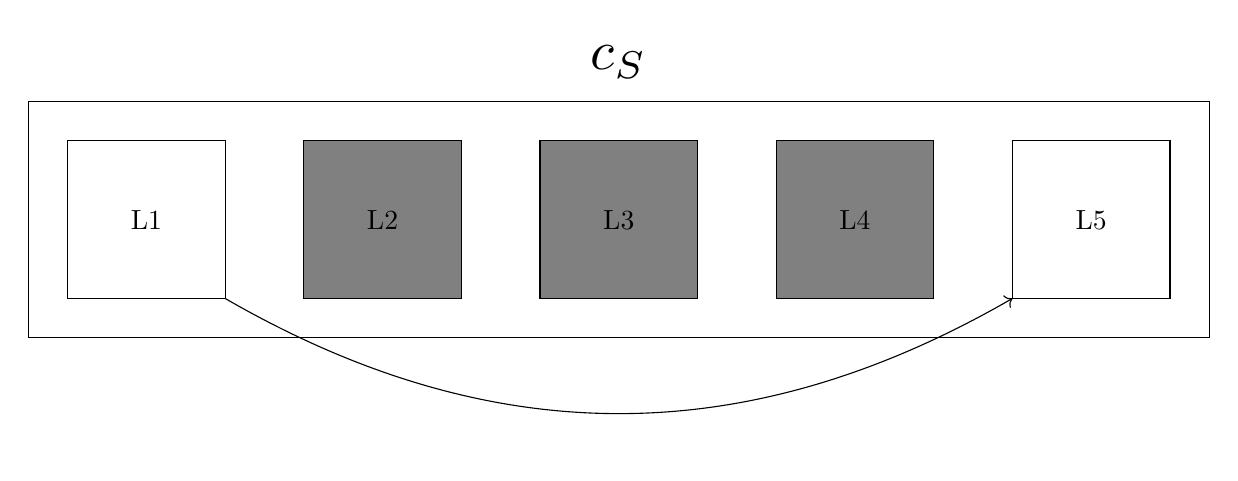
\begin{tikzpicture}
    \draw[fill=white!50] (0, 0) rectangle (2, 2);
    \node[anchor=center] at (1, 1) {L1};

    \draw[fill=black!50] (3, 0) rectangle (5, 2);
    \node[anchor=center] at (4, 1) {L2};

    \draw[fill=black!50] (6, 0) rectangle (8, 2);
    \node[anchor=center] at (7, 1) {L3};

    \draw[fill=black!50] (9, 0) rectangle (11, 2);
    \node[anchor=center] at (10, 1) {L4};

    \draw[fill=white!50] (12, 0) rectangle (14, 2);
    \node[anchor=center] at (13, 1) {L5};

    \draw[->] (2, 0) to[bend right] (12, 0);

    \node[anchor=center, scale=2] at (7,3) {$c_S$};
    \draw[] (-0.5, -0.5) rectangle (14.5, 2.5);
\end{tikzpicture}
    }
    \caption{Interpolation model learns to fill masked latents $m \circ z$ (L2, L3, L4) in between two keyframes latents (L1, L5) with context guidance.}
\end{figure}

\textbf{Context guidance \& Masking:} the model can be conditioned on context information, and is denoted with $c_S$ in figure \ref{fig:video_ldm_spatial_temporal_mixing_layers}. For long video synthesis, the model is conditioned on the initial set of $S$ context frames, which are the frames at the beginning of the clip. A temporal binary mask is applied to the frames that the model must predict, so the model knows which frames it must predict and which is the context guidance. The latent vector generated by the encoder is concatenated with the binary mask, forming the context guidance $c_S$.

\textbf{Temporal binary mask:} generating latents and turning them into video (temporal autoregressive is frame-by-frame prediction) is efficient, but it reaches its limits when generating long duration videos. In order to adapt to longer duration videos, the researchers trained models as \textit{prediction models} where for each two keyframes, interpolate between them (divide and conquer). By using \textbf{binary masks} $m_S$ (0 or 1) it indicates the model which frames and the context ($m = 1$) and which frames are to be predicted $m = 0$. The frames are multiplied by the mask and the model learns to predict the missing frames.

\textbf{Higher frame rate:} to achieve high frame rate (high temporal resolution), they predict three interpolated frames between each two keyframes; they call this $T \rightarrow 4T$ \textbf{interpolation model}. Its possible to achieve higher frame rates; its also possible to train $4T \rightarrow 16T$ interpolation model. They use the same interpolation model twice in order to further increase the frame rate.

\textbf{LDM Decoder: } after the interpolation models, the latents are then decoded to pixel space using the LDM decoder.

\textbf{Upsampler (L)DM: } to increase the spatial resolution of generated frames, they used a super-resolution (SR) model, which increases the output resolution by $4 \times $. They take inspiration from cascaded DMs \cite{cascaded_diffusion_models}, which we already discussed in Imagen (the SR3 model \cite{sr3}). In their experiments they used \textbf{pixel-space DM}, whereas for text-to-video models they used \textbf{LDM upsampler}. This step is optional, since its just for increasing the resolution of the generated video. However, since upsampling video frames independently would result in poor temporal consistency, they made the SR model video-aware by adding temporal layers and mixing spatial and temporal layers, in similar manner as discussed before.

\textbf{Number of parameters: } the Video-LDM model (except for the CLIP text encoder) consists of 3.1 billion parameters (autoencoder and diffusion models), and only 2.2 billion of these parameters are actually trained:

\begin{itemize}
    \item 84 million parameters in the autoencoder
    \item 865 million parameters in the image backbone LDM, not including CLIP text encoder
    \item 655 million parameters in temporal layers
    \item 354 million parameters in the text encoder (OpenCLIP-ViT/H)
    \item 1.5 million parameters in the interpolation latent diffusion model
\end{itemize}

Compared to Imagen (11.6 billion parameters) and CogVideo (9 billion parameters), Video-LDM is much smaller yet produced high quality videos, because it works in latent space.

\textbf{DDIM Sampling:} in appendix F of the paper they write that they use the sampler from denoising diffusion implicit models (DDIM) \cite{ddim} (section \ref{subsec:ddim_sampler}), where the stochastically $\eta$ is varied, as well as the guidance scale.

\textbf{CLIP text encoder: } the text encoder (for text-to-video model conditioning) is CLIP \cite{openai_clip} based which is used to generate text embeddings, as we discussed before (section \ref{subsec:clip}).










\subsection{Experiments}

\begin{figure}
    \centering
    \includegraphics[width=0.5\textwidth]{images/video_ldm/videoldm_vs_lvg_on_rds.png}
    \caption{\textit{Left}: Comparison of Video-LDM and Long Video GAN (LVG) on RDS dataset. \texttt{Cond.} means the model was conditioned on day/night and crowdedness. Side note: adding conditional information reduces FID and FVD. \textit{Right}: FVD and FID evaluations on different diffusion architectures (pixel-space diffusion model, end-to-end LDM that was not pre-trained on images [which is why the results are bad], and attention-only temporal model). Their model uses 3D temporal convolutions which is better than the attention-only diffusion model.}
    \label{fig:video_ldm_vs_lvg_on_rds}
\end{figure}

\begin{figure}
    \centering
    \includegraphics[width=0.7\textwidth]{images/video_ldm/rds.png}
    \caption{Real driving videos (RDS) generation samples. \textit{Top}: night videos. \textit{Middle:} the left red frame is the condition input, while the right is two different generated samples (given a frame, the model can generate the next frames). \textit{Bottom}: they trained a seperate bounding-box conditioned LDM for image synthesis only (the RDS dataset has some bounding-box clips), which generates initial frame (in yellow), and then Video-LDM completes the video generation based on this frame.}
\end{figure}

\begin{figure}
    \centering
    \includegraphics[width=0.7\textwidth]{images/video_ldm/webvid_samples.png}
    \caption{Generated samples at $1280\times 2048$ resolution trained on WebVid-10M dataset. Prompts: "An astronaut flying in space, 4k, high resolution" and "Milk dripping into a cup of coffee, high definition, 4k".}
\end{figure}

\begin{figure}
    \centering

    \begin{subfigure}{0.45\textwidth}
        \centering
        \includegraphics[width=0.8\linewidth]{images/video_ldm/ucf.png}
        \caption{UCF-101 dataset. Video-LDM achieves the best inception score.}
    \end{subfigure}

    \begin{subfigure}{0.45\textwidth}
        \centering
        \includegraphics[width=0.8\linewidth]{images/video_ldm/msr_vtt.png}
        \caption{MSR-VTT dataset. Video-LDM almost achieves the best CLIP-SIM score.}
    \end{subfigure}

    \caption{Zero-shot text-to-video synthesis on UCF-101 and MSR-VTT datasets. Video-LDM is compared to other state-of-the-art models in zero-shot setting.}
\end{figure}




The researchers used the following datasets:

\begin{itemize}
    \item In-house dataset of real driving videos (RDS). The dataset consists of 683,060 videos up to 8 seconds long at 512x1024 resolution, and frame rate up to 30 fps. The dataset has day and night driving videos, annotation of number of vehicles ("crowdedness") and some of them even have bounding boxes of cars. They conditioned on day/night labels and crowdedness and randomly dropped these labels during training to allow for classifier-free guidance and unconditional synthesis. The previous state-of-the-art model in terms of long-term high-resolution video synthesis was Long Video GAN (LVG) \cite{brooks2022generating} is compared to Video-LDM on the same dataset in figure \ref{fig:video_ldm_vs_lvg_on_rds}.
    \item WebVid-10M dataset \cite{webvid_10m} that contains 10.7 million video-caption pairs with total of 52K hours. For this experiment, they turned a publicly available Stable Diffusion model into a text-to-video synthesis model by adding temporal alignment layers. First, they fine-tuned the spatial layers on frames from the dataset and only then insert the temporal layers. Then, they freeze the spatial layers and train only the temporal layers on WebVid-10M videos with the addition the caption (text) of the dataset. In similar manner, they fine-tuned the Stable Diffusion upsampler which can upscale by $4\times$ the frames and generate videos at $1280\times 2048$ resolution (the dataset clips resolution is $320\times 512$). The samples are 113 frames, which translates either to 4.7 second @ 24 fps or 3.8 seconds @ 30 fps.
    \item Mountain bike dataset \cite{brooks2022generating} which was introduced by Long Video GAN paper consists of 1,202 video clips of varying, but at least 5 seconds length at 30 fps. Details and samples are in the Video-LDM paper.
\end{itemize}

\textbf{Evaluation metrics: } they used FID to evaluate quality of individual frames. They also used FVD and human evaluation on video clips compared to LVG: it was a user study, 100 videos @ 4 seconds, given pair of videos (one from Video-LDM and one from LVG), and participants select the most favorable. For text-to-video model, they evaluated CLIP similarity (CLIP-SIM), and also inception score. They used the ViT-B/32 \cite{openai_clip} model by OpenAI to compute the CLIP score.

In their experiments they \textbf{successfully generated very long temporally coherent high-resolution driving videos of multiple minutes (up to 5 minutes long!)}.

\textbf{Video synthesis on RDS dataset: } for video synthesis on RDS dataset, they first generate a single frame using the image LDM, then they run the prediction model on a \textbf{single frame}, to generate a sequence of key frames. Then, they call the prediction model again, but condition on \textbf{two frames}. Next they optionally perform two steps of the interpolation model which increases the FPS from 1.875 to 7.5 and from 7.5 to 30 fps. And then, optionally they run the patch-wise upsampler which is run over portions of 8 video frames (the upsampler is also temporally aligned).

\section{Imagen-Video}
\label{sec:imagen_video}

\begin{figure}
    \centering
    \includegraphics[width=0.7\textwidth]{images/video_synthesis/imagen_video.png}
    \caption{Imagen-Video video samples \cite{imagen_video}.}
\end{figure}

\begin{figure}
    \centering
    \includegraphics[width=0.7\textwidth]{images/imagen_video/pipeline.png}
    \caption{The cascading pipeline of Imagen-Video. The text embeddings are injected to all models in the pipeline (not shown) \cite{imagen_video}.}
    \label{fig:imagen_video_pipeline}
\end{figure}

Imagen-Video by Google \cite{imagen_video} is a T2V cascading diffusion model, based on Imagen (section \ref{sec:imagen}). Imagen-Video has 7 sub-models in a cascading pipeline (figure \ref{fig:imagen_video_pipeline}). It generates high definition $1280\times 768$ videos @ 24 fps, for 5.3 seconds. A big downside compared to Video-LDM is that Imagen-Video works in the pixel-space, whereas Video-LDM works in latent space. In addition, Imagen-Video is a much larger model and uses more compute resources than Video-LDM, however Google is able to achieve good scaling results through training on massive datasets.

Like Imagen, Imagen-Video uses the same large frozen text-encoder T5-XXL (section \ref{subsec:t5}) in its pipeline. The benefit of cascading pipeline is the ability to independently train each model, allowing the parallel training of all 7 models.

\begin{figure}
    \centering
    \includegraphics[width=0.7\textwidth]{images/imagen_video/video_u_net.png}
    \caption{Video U-Net block \cite{video_diffusion_models} used by Imagen-Video \cite{imagen_video}.}
    \label{fig:imagen_video_video_unet}
\end{figure}


Imagen Video also builds on the work of \textbf{Video U-Net} \cite{video_diffusion_models}, which generalizes the 2D diffusion model architecture to 3D in space-time by using temporal attention and 3D convolution layers to capture dependencies between video frames. See figure \ref{fig:imagen_video_video_unet}.

Due to safety and ethical concerns in training the Imagen-Video model, the researchers \textbf{decided not to release the model to the public} and keep it closed source.

One of the contribution of the paper is that they successfully transferred multiple methods from the image domain to video, such as \textbf{v-parameterization \cite{v_prediction}, CFG and conditioning augmentation} \cite{cascaded_diffusion_models} (similar to Imagen). They also found out that \textbf{progressive distillation} \cite{v_prediction} \cite{meng2023distillation} is a valuable technique for speeding up video sampling.














\subsection{Architecture \& Method}

Imagen Video has one frozen text encoder (T5-XXL), one base video diffusion model, three SSR (spatial super-resolution) models, and three TSR (temporal super-resolution) models - totaling 7 video diffusion models. Each of the denoising diffusion models $\hat{x_\theta}$ operate on multiple video frames simultaneously. In figure \ref{fig:imagen_video_video_unet} the spatial convolution and spatial attention operate on each frame independently, while temporal attention and convolution operate on a collection of frames.

Whereas typically diffusion models for image generation use a 2D U-Net architecture (spatial attention and convolution), \textbf{Video U-Net} block used by Imagen-Video (figure \ref{fig:imagen_video_video_unet}) generalizes the U-Net to 3D space-time by using temporal attention and convolution to capture dependencies between video frames.

Imagen-Video pipeline is compromised of the following model types:

\begin{itemize}
    \item \textbf{T5-XXL}: T5-XXL is a text-to-text transformer used to encode the text prompts to embeddings which are then used to condition all of the 7 diffusion models.
    \item \textbf{Base}: The base diffusion model generate low FPS low resolution video clip.
    \item \textbf{SSR}: The SSR model is a spatial SR (SSR) model that increases the resolution of the input image. Unlike the base model, it uses temporal convolution instead of temporal attention. Like SR3, we first apply bilinear or bicubic interpolation to increase the resolution, then we remove noise (add details) by first concatenating noise $y_t$ to the upsampled image $x$ and then use the U-Net denoising network to learn to denoise the image.
    \item \textbf{TSR}: The TSR model is a temporal SR (TSR) model that increases the temporal resolution of the input video (increases frame count) by frame interpolation. This model also uses temporal convolution instead of temporal attention.
\end{itemize}

\textbf{Temporal Attention v.s. Temporal Convolution}: Temporal convolution reduces memory and computation costs over temporal attention, which is critical for the SSR and TSR models, because they are applied to high-resolution high-fps videos. This is why temporal attention is used at the beginning of the cascading pipeline.

\textbf{Spatial attention at the beginning of the pipeline}: The base model and the first two SSR models have spatial attention in addition to spatial convolution, because spatial attention at the beginning of the pipeline requires less compute resources than at the end. The last SSR model in the pipeline is a fully convolutional model (without attention).

\textbf{Number of parameters}: Imagen-Video consists of 11.6 billion parameters. Each of the model's parameters count is shown in figure \ref{fig:imagen_video_pipeline}.

\textbf{Classifier-free guidance}: CFG is also used in Imagen-Video. They found that it helps the model generate high fidelity samples with respect to the text prompts. Higher guidance weights lead the model to focus more on the text prompt conditioning.

\textbf{Oscillating guidance}: Similar to Imagen, when the guidance weight is too large, the possible range of values of predicted noise is beyond $[-1, 1]$, which causes train-test mismatch. This leads to significant artifacts in the generated videos. \textbf{Dynamic thresholding}, as described in section \ref{subsec:imagen_diffusion_guidance_weight}, helps to prevent this issue, which dynamically clip the image to the chosen threshold followed by scaling by $s$: \texttt{np.clip(x, -s, s) / s}. However, a constant high guidance weight leads to saturation artifacts, especially at high resolutions. The researchers didn't find dynamic thresholding sufficient, and they experimented with letting the guidance weight \textbf{oscillate between high and low values} (min and max) for a certain number of sampling steps. They apply this \textbf{oscillating dynamic threshold} only to the base and first SR models. The generation starts with a high guidance weight to establish a strong alignment with the prompt, then alternates between high and low weights in subsequent steps.

\textbf{Noise conditioning augmentation}: Similar to Imagen, Imagen-Video applied noise conditioning augmentation for all the spatial and temporal diffusion models. Noise conditioning augmentation is used to \textbf{corrupt low-resolution images}, and then the \textbf{SR model would be conditioned on the noise level}. The corruption noise level ("\textbf{augmentation level}") helps the model to generalize better to various noise levels and improves the diversity and quality of samples. This technique was introduced in a 2021 paper \cite{cascaded_diffusion_models} by Google.







\subsection{Video-image joint training}

Training on both images and videos improves fidelity and enables knowledge transfer from images to videos, addressing the scarcity of text-video pairs datasets. This approach allows the model to learn diverse video styles.

Imagen-Video adopts the joint training method from \cite{video_diffusion_models}, treating individual images as single-frame videos. To exclude temporal components during image training, they mask the temporal computation paths, preventing temporal operations across frames.




















\subsection{v-prediction}

v-prediction (velocity prediction) is a parameterization strategy used in diffusion models to predict the change of pixels in time of the diffusion process. Unlike $\epsilon$-prediction, which the U-Net predicts the noise, v-prediction predicts the change of noise. There is also $x$-prediction in which the U-Net predicts the clean, original data $x_t$ at timestep $t$ instead of the noise added.

v-prediction is defined as:

\[ v \equiv \alpha_t \epsilon - \sigma_t x \]

where $\alpha_t$ is the time-dependent coefficient determined by noise scheduler, $\epsilon$ is the noise, $x$ is the data, and $\sigma_t$ is the standard deviation of the noise at timestep $t$.
















\subsection{Progressive distillation with guidance and stochastic samplers}

In a 2022 paper by Google \cite{v_prediction}, the team introduced \textbf{progressive distillation}, a fast sampling method for diffusion models. Unlike traditional DDPM samplers, requiring thousands of steps, progressive distillation enables sampling in a fixed, reduced number of steps. By iteratively distilling a DDIM sampler (see section \ref{subsec:ddim_sampler}), the required steps are halved with each distillation. This method is used with v-prediction.

\begin{figure}
    \centering
    \includegraphics[width=0.6\textwidth]{images/imagen_video/v_prediction.png}
    \caption{Progressive distillation process \cite{v_prediction}.}
    \label{fig:progressive_distillation}
\end{figure}

In figure \ref{fig:progressive_distillation} we see the distillation process: instead of taking 4 sampler steps ($f(z; \eta)$) to transform noise $\epsilon$ to an image $x$, the distilled model now takes a single step.

In progressive distillation we duplicate a model that we desire to distill, which becomes a "student" and "teacher" model (they start with the same weights and biases). The student model learns to produce the output of the teacher model in fewer steps. The teacher model uses two steps of DDIM sampling and the student should learn to output the same teacher's output but in a single sampling step.

\begin{figure}
    \centering
    \includegraphics[width=0.7\textwidth]{images/imagen_video/progressive_distillation.png}
    \caption{Progressive distillation algorithm \cite{v_prediction}. }
    \label{fig:progressive_distillation_algorithm}
\end{figure}







\begin{algorithm}
    \caption{Standard diffusion training algorithm \cite{v_prediction}}
    \begin{algorithmic}
        \Require Model $\hat{\mathbf{x}}_{\theta}(\mathbf{z}_t)$ to be trained
        \Require Data set $\mathcal{D}$
        \Require Loss weight function $w()$
        
        \While{not converged}
            \State $\mathbf{x} \sim \mathcal{D}$ \Comment{Sample data}
            \State $t \sim U[0,1]$ \Comment{Sample time}
            \State $\epsilon \sim \mathcal{N}(0, I)$ \Comment{Sample noise}
            \State $\mathbf{z}_t = \alpha_t \mathbf{x} + \sigma_t \epsilon$ \Comment{Add noise to data}
            
            \State $\tilde{\mathbf{x}} = \mathbf{x}$ \Comment{Clean data is target for $\hat{\mathbf{x}}$}
            \State $\lambda_t = \log[\alpha_t^2/\sigma_t^2]$ \Comment{log-SNR}
            \State $L_{\theta} = w(\lambda_t) \|\tilde{\mathbf{x}} - \hat{\mathbf{x}}_{\theta}(\mathbf{z}_t)\|_2^2$ \Comment{Loss}
            \State $\theta \gets \theta - \gamma \nabla_{\theta} L_{\theta}$ \Comment{Optimization}
        \EndWhile
    \end{algorithmic}
\end{algorithm}
    






\begin{algorithm}
    \caption{Progressive distillation algorithm \cite{v_prediction}}
    \begin{algorithmic}
        \Require \colorbox{lime} {Trained teacher model $\hat{\mathbf{x}}_{\eta}(\mathbf{z}_t)$}
        \Require Data set $\mathcal{D}$
        \Require Loss weight function $w()$
        \Require \colorbox{lime}{Student sampling steps $N$}
        \For{\colorbox{lime}{$K$ iterations}}
            \State \colorbox{lime}{$\theta \gets \eta$} \Comment{Init student from teacher}
            \While{not converged}
                \State $\mathbf{x} \sim \mathcal{D}$
                \State \colorbox{lime}{$t = i/N, \quad i \sim \text{Cat}[1,2,\dots,N]$}
                \State $\epsilon \sim \mathcal{N}(0, I)$
                \State $\mathbf{z}_t = \alpha_t \mathbf{x} + \sigma_t \epsilon$
                
                \State \colorbox{lime}{{\textbf{\# 2 steps of DDIM with teacher}}}
                \State \colorbox{lime}{{$t' = t - 0.5/N, \quad t'' = t - 1/N$}}
                \State \colorbox{lime}{{$\mathbf{z}_{t'} = \alpha_{t'} \hat{\mathbf{x}}_{\eta}(\mathbf{z}_t) + \frac{\sigma_{t'}}{\sigma_t} (\mathbf{z}_t - \alpha_t \hat{\mathbf{x}}_{\eta}(\mathbf{z}_t))$}}
                \State \colorbox{lime}{{$\mathbf{z}_{t''} = \alpha_{t''} \hat{\mathbf{x}}_{\eta}(\mathbf{z}_{t'}) + \frac{\sigma_{t''}}{\sigma_{t'}} (\mathbf{z}_{t'} - \alpha_{t'} \hat{\mathbf{x}}_{\eta}(\mathbf{z}_{t'})$)}}
                \State \colorbox{lime}{{$\tilde{\mathbf{x}} = \frac{\mathbf{z}_{t''} - (\sigma_{t''}/\sigma_t) \mathbf{z}_t}{\alpha_{t''} - (\sigma_{t''}/\sigma_t) \alpha_t}$}} \Comment{Teacher $\hat{\mathbf{x}}$ target}
                
                \State $\lambda_t = \log[\alpha_t^2/\sigma_t^2]$
                \State $L_{\theta} = w(\lambda_t) \|\tilde{\mathbf{x}} - \hat{\mathbf{x}}_{\theta}(\mathbf{z}_t)\|_2^2$
                \State $\theta \gets \theta - \gamma \nabla_{\theta} L_{\theta}$
            \EndWhile
            \State \colorbox{lime}{$\eta \gets \theta$} \Comment{Student becomes next teacher}
            \State \colorbox{lime}{$N \gets N/2$} \Comment{Halve number of sampling steps}
        \EndFor
    \end{algorithmic}
\end{algorithm}
    










This process is illustrated in figure \ref{fig:progressive_distillation_algorithm}. The teacher model $\hat{x}_{\eta} (z_t)$ is the diffusion model $\hat{x}_{\theta} (z_t)$ where $z_t$ is the noisy data (we take training data $\mathcal{D}$ and add noise to it). After the student model (with parameters $\eta$) learns to predict $\tilde{x}$ (which is two DDIM steps), is distilled to match the output of the teacher model. Then the teacher model becomes the student and the process is repeated.

\begin{figure}
    \centering
    \includegraphics[width=0.6\textwidth]{images/imagen_video/samplers_comparison.png}
    \caption{Comparison of v-prediction sampling to DDIM and stochastic samplers. The distilled model achieves significant lower FID scores with significantly fewer sampling steps (converges faster) \cite{v_prediction}.}
    \label{fig:samplers_comparison}
\end{figure}

We can see in figure \ref{fig:samplers_comparison} that using a distilled model, sampling takes significantly fewer steps to converge to the same quality as the DDIM or stochastic (DDPM) samplers.

\begin{figure}
    \centering
    \includegraphics[width=0.7\textwidth]{images/imagen_video/e_prediction_vs_v_prediction.png}
    \caption{$\epsilon$-prediction (middle row) v.s. v-prediction (bottom row). In $\epsilon$-prediction we see color shifts across frames, whereas v-prediction is more consistent \cite{imagen_video}.}
    \label{fig:imagen_video_epsilon_prediction_vs_v_prediction}
\end{figure}

At higher resolutions, v-prediction avoids temporal color shifting artifacts compared to $\epsilon$-prediction. We can see that in figure \ref{fig:imagen_video_epsilon_prediction_vs_v_prediction}. The researchers say the reason is that in distillation we have to work at higher noise levels to the point where the signal-to-noise ratio (SNR) drops down to zero, at which point predicting the noise becomes a lot harder.













\subsubsection*{Distillation with classifier-free guidance}

The paper \cite{meng2023distillation} by Google Research and Stability AI extends \cite{v_prediction} by applying distillation to models trained with CFG, marking its first use in video domain. In this work, the teacher model (trained with CFG, before distillation) takes two DDIM steps, and the student model, denoted in the paper as a $w$-conditioned model, learns to match the teacher's output while being conditioned on the guidance scale. This conditioning incorporates the guidance weight into the model backbone, similar to timestep conditioning in \cite{kingma2021variational}. The student model is optimized with the following objective \cite{meng2023distillation}:

\begin{equation*}
\mathbb{E}_{w \sim p_w, t \sim U[0, 1], x \sim p_{\text{data}}(x)} 
\left[ 
    \omega(\lambda_t) \left\| 
        \underbrace{\hat{x}_{\eta_1}(z_t, w)}_{\text{student's pred}} - 
        \underbrace{\hat{x}_{\theta}^w(z_t) }_{\text{teacher's pred}}
    \right\|_2^2 
\right]
\end{equation*}

where:

\begin{itemize}
    \item $w$ is the guidance weight and is picked from $p_w$: $w \sim p_w$ (which can be fixed or oscillate, but in Imagen-Video they chose to oscillate)
    \item $p_w(w) = U[w_{\text{min}}, w_{\text{max}}]$ is the oscillating guidance weight function
    \item $t$ is the diffusion timestep
    \item $x$ is the data (images): $x \sim p_{\text{data}}(x)$
    \item $z_t$ is the noised version of $x$ (noisy image at timestep $t$)
    \item $\lambda_t$ is the guidance scale (not really important)
    \item $\omega(\lambda_t)$ is the weighting function (also not really important)
    \item $\hat{x}_{\eta_1}$ is the student model (which is conditioned on the guidance weight $w$ as input: $\hat{x}_{\eta_1}(z_t, \textcolor{red}{w})$). Also notice the notation: $\hat{x}_{\eta_\mathbf{\textcolor{red}{1}}}$, which means that this is the first distillation iteration.
    \item $\hat{x}_{\theta}^w$ is the teacher model. Notice in the notation, its using the guidance weight in CFG (its not given as input): $\hat{x}_{\theta}^\mathbf{\textcolor{red}{w}}(z_t)$
\end{itemize}

Also notice that the teacher model's parameters ($\eta$) are different to the student model's parameters ($\theta$), since they change at each distillation step (the student is a copy of the teacher but to differentiate between the parameters after the distillation process they chose to differentiate the parameters notations).

In the \cite{meng2023distillation} paper we optimize the student's objective:

\[  
    \hat{x}_{\theta}^w(z_t) = 
    \underbrace{(1+w) \hat{x}_{c,\theta} (z_t)}_{\text{conditional score}} - 
    \underbrace{w \hat{x}_\theta (z_t)}_{\text{unconditional score}}
\]

where $c$ is the teacher model's conditioning (for example, text prompt) \footnote{Thanks to \href{https://www.youtube.com/watch?v=ZXuK6IRJlnk}{this youtube tutorial} for explaining both papers}.

To summarize, Using the work of \cite{meng2023distillation}, Imagen-Video researchers successfully distilled 7 video diffusion models with CFG to just 8 sampling steps without any noticeable loss in perceptual quality in the pipeline.

















\subsection{Experiments}

In their experiments, they sampled video clips at $192\times 320$ resolution @ 24 fps for 128 frames (5.3 seconds). They repeat the evaluations over four runs and report the mean and standard error.

\textbf{Datasets}: The researchers used 14 billion video-text pairs and 60 million image-text pairs from internal and public datasets, such as LAION-400M \cite{laion_400m}.

\textbf{Pre-processing}: They resized images using antialiased bilinear resizing and temporally resize videos by skipping frames.

\textbf{Evaluation}: They used FID on individual video frames, FVD for video, and frame-wise CLIP scores for video-text alignment (they take the average across all frames).

\begin{figure}
    \centering
    \includegraphics[width=0.8\textwidth]{images/imagen_video/scaling.png}
    \caption{Imagen-Video scaling results on video U-Net. The more parameters the model has, the better the FVD and CLIP scores \cite{imagen_video}.}
    \label{fig:imagen_video_scaling}
\end{figure}

\textbf{Scaling}: In figure \ref{fig:imagen_video_scaling} we can see interesting result which contradicts the findings of Imagen \cite{imagen} paper. They found that increasing the U-Net size doesn't scale the sample quality as much as increasing the text encoder size. They conclude that video modeling task for which the performance is not yet saturated at current model sizes \footnote{This finding could hint that transformers, which benefit from scaling on large datasets, could provide the necessary scaling capabilities that video modeling task demands.}.

\begin{figure}
    \centering
    \includegraphics[width=0.5\textwidth]{images/imagen_video/e_prediction_vs_v_prediction_2.png}
    \caption{$\epsilon$-prediction v.s. v-prediction parameterization. v-prediction converges faster \cite{imagen_video}.}
\end{figure}

\begin{figure}
    \centering
    \includegraphics[width=0.6\textwidth]{images/imagen_video/experiments_table.png}
    \caption{Testing of fixed and oscillating guidance weight, distillation of base and SR models and evaluating each pipeline on CLIP score and sampling time. Distilling the pipeline results in significantly faster sampling time, while oscillating guidance weight improves the CLIP score a little \cite{imagen_video}.}
    \label{fig:imagen_video_experiments_table}
\end{figure}

\textbf{Quality vs. Sampling time in a distilled model}: In figure \ref{fig:imagen_video_experiments_table} we can see that distillation provides a good trade-off between sampling time and quality. Distilled model is 18x times faster in sampling, without significant degradation in perceptual quality. IIn addition, the distilled model is also 36x more efficient in terms of compute cost in FLOPs metric. 


\section{Make-a-Video}
\label{sec:make_a_video}

Make-a-Video \cite{make_a_video} (2022) by Meta AI is a text-to-video model. Similar to Video-LDM, Make-a-Video extends the text-to-image (T2I) knowledge to diffusion-based text-to-video (T2V) model through spatiotemporally factorized diffusion model. In addition, it \textbf{doesn't require pairs of text-video data}, which allows unsupervised video training, which in turn allows to scale to larger quantities of video data.

They present super-resolution strategies in space and time to generate higher spatial-resolution and higher frame rate video clips, provided a text prompt. They \textbf{leverage image priors} due to the complexity of modeling videos, which simplifies the learning process.

The model has 3 main stages:

\begin{itemize}
    \item \textbf{Training a T2I model on text-image pairs}. This model is variation of DALL-E 2 \cite{dalle_2} (section \ref{sec:dalle_2}) by OpenAI.
    \item Converting the T2I model to T2V model by \textbf{adding 3D convolutions and temporal attention layers in the U-Net}, so the model can understand video data. It becomes a T2V model.
    \item \textbf{Unsupervised training of the T2V model on video data} (no text-to-video data is needed), which is very attractive.
\end{itemize}



\subsection{Architecture \& Method}

\begin{figure}
    \centering
    \includegraphics[width=1\textwidth]{images/make_a_video/overview.png}
    \caption{Make-a-Video model high-level architecture overview (after adding temporal layers). The T2I model doesn't have "fps" input, the decoder generates only a single image, there is no interpolation network, and has two spatial-super-resolution networks, and no spatio-temporal super-resolution network, since in image we don't deal with the temporal axis.}
    \label{fig:make_a_video_overview}
\end{figure}

In figure \ref{fig:make_a_video_overview}:

\begin{itemize}
    \item The model input is text prompt $x$ and "fps" (frames per second).
    \item The \textbf{CLIP text encoder} $C_x$ (not shown in the figure) is used to translate the text prompt $x$ into text embeddings $x_e$, which are fed to the prior network $\textcolor{Maroon}{P}$.
    \item The \textbf{image embedding prior} $\textcolor{Maroon}{P}$ translates these text embeddings $x_e$ into image embeddings $y_e$.
    \item The \textbf{spatio-temporal decoder $\textcolor{blue}{D^t}$} generates 16 $64\times 64$ frames, conditioned on these image embeddings $y_e$.
    \item These 16 images are interpolated into higher fps by the \textbf{frame interpolation model $\textcolor{OliveGreen}{\uparrow_F}$}, through masked interpolation prediction, as we saw in previous papers.
    \item Then these frames are increased in spatial resolution to $256\times 256$ by the \textbf{spatiotemporal super-resolution model $\textcolor{Plum}{SR_l^t}$}.
    \item And finally increased to resolution $768\times 768$ by \textbf{spatial super-resolution model $SR_h$}. The final output is high-spatiotemporal-resolution video $\hat{y}$.
\end{itemize}

The formal mathematical formulation of the Make-a-Video inference is as follows:

\begin{equation}
    \hat{y_t} = \text{SR}_h \circ \textcolor{Plum}{\text{SR}_l^t} \circ \textcolor{OliveGreen}{\uparrow_F} \circ \textcolor{blue}{D^t} \circ \textcolor{Maroon}{P} \circ \left( \hat{x}, C_x (x) \right)
    \label{eq:make_a_video_inference}
\end{equation}

where $\hat{x}$ is the BPE encoded text tokens.







\subsection{The T2I model}

The T2I model is based on the core components of the OpenAI paper \cite{dalle_2}. In this paper, OpenAI created a model that is called unCLIP (commonly known as DALL-E 2). See section \ref{sec:dalle_2} for more details. They first trained the T2I model, and only then they apply factorization on the T2I model to create the T2V model. We will discuss this T2I model here and in the next section, and explain how they transfer this spatial knowledge to video in section \ref{sec:make_a_video_expanding_t2i_to_video}.

The researchers note that after the inference (equation \ref{eq:make_a_video_inference}), they then downsample the image to $512\times 512$ using bicubic interpolation for cleaner aesthetics.







\subsubsection{DALL-E 2}
\label{sec:dalle_2}

DALL-E 2 by OpenAI \cite{dalle_2} is a diffusion-based T2I model, which leverages contrastive models like CLIP for image generation. They proposed a two-stage model: 

\begin{itemize}
    \item a prior network $P(z_i | y)$ that generates CLIP image embeddings $z_i$ conditioned on captions
    \item and a diffusion based decoder $P(x | z_i, y)$ that generates images $x$ conditioned on these image embeddings $z_i$, and optionally the captions $y$.
\end{itemize}

\begin{figure}
    \centering
    \includegraphics[width=0.7\textwidth]{images/make_a_video/dalle_2.png}
    \caption{High level overview of unCLIP (DALL-E 2) \cite{dalle_2} by OpenAI. The top figure shows the training objective of DALL-E 2, and the bottom figure shows the inference process. The prior model takes the CLIP text embeddings $z_t$ and generates image embeddings $z_i$. Then the decoder takes in image embeddings $z_i$ and generates the final image.}
    \label{fig:make_a_video_dalle2_overview}
\end{figure}

In figure \ref{fig:make_a_video_overview}, we can see the training objective of DALL-E 2 and the inference process. The decoder acts as inverted CLIP encoder. Given inputs $(x, y)$ where $x$ are images and $y$ are their caption, then $z_i$ is the corresponding CLIP image embeddings and $z_t$ is the CLIP text embeddings.

\begin{itemize}
    \item \textbf{Input}: the training dataset is pairs $(x,y)$ of images $x$ and captions $y$.
    
    \item \textbf{Output}: a generated image $x$ given a caption $y$.

    \item \textbf{CLIP encoder} is applied to the text $x$ and caption $y$ to get text and image embeddings $z_i$ and $z_t$ respectively.
    
    \item \textbf{Training objective}: the text embedding $z_t$ (the blue vector in figure \ref{fig:make_a_video_overview}) should match the CLIP image embeddings $z_i$ (the brown vector in figure \ref{fig:make_a_video_overview}).
    
    \item \textbf{The prior network} maps the text embeddings $z_t$ to a \textit{distribution} of possible image embedding vectors $z_i$. In their experiments, they tried two different prior networks:
        \begin{itemize}
            \item \textbf{Autoregressive} prior: the image embedding $z_i$ is converted to a sequence of discrete codes and predicted autoregressively conditioned on the caption $y$. This network is based on the transformer architecture.
            \item \textbf{Diffusion} based prior where the latent vector $z_i$ is modeled using Gaussian diffusion model conditioned on caption $y$. The diffusion model is a decoder-only transformer, instead of a standard U-Net, similar to Diffusion Transformer \cite{diffusion_transformer}.
        \end{itemize}
    
    \item \textbf{Decoder network}: given image embeddings $z_i$, the unCLIP network generates the final image; the decoder is considered inverse of CLIP encoder, or just "unCLIP" (hence the name). They also used classifier-free guidance to improve the quality of the generated images.
    
    \item \textbf{Sampling in DALL-E}: to sample an image we need to first sample $z_i$ using the prior network, and then sample $x$ using the decoder (given $z_i$).
    
    \item \textbf{Super-resolution}: they also trained two SR diffusion-based networks to upsample the final generated image from $64\times 64$ to $256\times 256$ and finally to $1024\times 1024$.
\end{itemize}

\textbf{x-prediction}: In the prior network, instead of predicting the noise directly ($\epsilon$-prediction), they chose to predict the unnoised $z_i$ directly (called $x$-prediction).





\subsection{Expanding the T2I model to video domain}
\label{sec:make_a_video_expanding_t2i_to_video}

The researchers modify the T2I model and transfer the image knowledge to video domain by expanding the 2D conditional network into the temporal dimension.

In short, they support the temporal dimension by adding 3D convolutions temporal attention layers in the U-Net backbone of the T2I diffusion model. The \textbf{fully-connected layers doesn't need factorization since they are agnostic to structured spatial and temporal information}.



\subsubsection{Spatiotemporal layers}

The spatiotemporal decoder $\textcolor{blue}{D^t}$ now \textbf{generates 16 RGB frames} of $64\times 64$ resolution, instead of one frame.

They added a new network: \textbf{frame interpolation network} $\textcolor{OliveGreen}{\uparrow_F}$ which increases the fps by interpolating on the 16 frames from the spatiotemporal decoder (as seen in figure \ref{fig:make_a_video_overview}).

\textbf{Hallucination}: the super-resolution model involves hallucinating information. In order not to have flickering artifacts, the hallucination must be consistent across frames. As a result, $\text{SR}_l^t$ operates across spatial and temporal dimensions.

They also modified the spatial layers of the super-resolution network $\text{SR}_l$ to spatiotemporal super-resolution network $\textcolor{red}{\mathbf{\text{SR}_l^t}}$. \textbf{But chose not to operate in the temporal dimension} in $\text{SR}_h$. The reason being because of memory and compute constraints higher in the pipeline.

In order to consistent detail hallucination across frames, in $\text{SR}_h$ they use the same noise initialization for each frame.



\subsubsection{Pseudo-3D convolutional layers}

Because 3D convolutional layers are very compute and memory expensive, the researchers opt to go with pseudo 3D convolutional layers.

In \cite{chollet2017xception}, the authors proposed a method to replace 3D convolutions with pseudo-3D convolutions. In this method they decouple the processing of spatial and temporal dimensions, which they call "depthwise separable convolution layers". In Make-a-Video they say that in addition to the more compute efficient convolutions they also want to retain the previously learned spatial knowledge of the T2I model.

\textbf{First they apply the 2D convolution on spatial axis and only then they apply 1D convolution on the temporal axis}. This facilitates information sharing between the spatial and temporal axes.

The pseudo-3D convolutional layer is defined as:

\[ 
\text{Conv}_{\text{P3D}} (h) := \text{Conv}_{\text{1D}} (
    \text{Conv}_{\text{2D}} (h) \circ T
) \circ T \]

where $h \in \mathbb{R}^{B\times C\times F\times H\times W}$ is an input tensor, where $B,\ C,\ F,\ H,\ W$ are the batch, channels, frames, height and width respectively, and $\circ T$ is the transpose operator which swaps between spatial and temporal dimensions.

\begin{figure}
    \centering
    \includegraphics[width=0.7\textwidth]{images/make_a_video/pseudo_3d.png}
    \caption{Initialization and architecture of pseudo-3D convolutional and attention layers. Left: Pseudo-3D convolution and initialization. Right: Pseudo-3D attention and initialization.}
    \label{fig:make_a_video_pseudo_3d_conv_and_attention}
\end{figure}

\textbf{Spatiotemporal initialization}: In figure \ref{fig:make_a_video_pseudo_3d_conv_and_attention} we can see the pseudo-3D convolutional layer initialization. After applying 2D spatial convolutions they apply 1D temporal convolution. \textbf{The temporal 1D convolution layer is initialized as the identity function, it performs no transformation on the input data initially}. This way the network relies on the already learned spatial features. \textbf{The temporal consistency will be learned at a later stage}, where the model is trained on video dataset.






\subsubsection{Pseudo-3D attention layers}

Adding the temporal dimension to the attention layers is computationally infeasible. They follow the work of \cite{video_diffusion_models} (Video U-Net), similar to how \textbf{Imagen-Video} works (in Imagen-Video paper they also mentioned that they use the work of Video U-Net).

After each pre-trained spatial attention layer they stack a pseudo-3D temporal attention layer. 

Given tensor a tensor $h$ the \texttt{flatten} operation flattens the spatial dimension to: 

\[ 
h' \in \mathbb{R}^{B\times C\times F\times \mathbf{\textcolor{red}{HW}}} 
\] 

and \texttt{unflatten} operation is the inverse operation. The pseudo-3D attention layer is defined as:

\[ \text{ATTN}_{\text{P3D}} (h) = \text{unflatten} 
(\text{ATTN}_{\text{1D}} 
(\text{ATTN}_{\text{2D}} 
(\text{flatten} (h)) \circ T) \circ T) 
\]

\textbf{Spatiotemporal initialization}: To allow for smooth spatiotemporal initialization, $\text{ATTN}_{\text{2D}}$ is initialized from the pre-trained T2I model and the $\text{ATTN}_{\text{1D}}$ is initialized as the identity function (see figure \ref{fig:make_a_video_pseudo_3d_conv_and_attention}).

\textbf{FPS conditioning}: similar to \cite{cogvideo}, they added additional conditioning parameter $\text{fps}$, which enables additional augmentation method that deals with limited volume of training videos and provides more control over the generated video at inference time.





\subsection{Frame interpolation network}

The frame interpolation network $\textcolor{OliveGreen}{\uparrow_F}$ increases number of frames by interpolation or pre/post extrapolation. In addition to RGB channels, they add the binary mask channel (0 or 1) indicating which frames masked during training on masked interpolation. The model is conditioned on $\text{fps}$ which enable multiple temporal upsample rates at inference. For extrapolation, they can use the same strategy.




\subsection{Training}

The prior network is trained on text-image pairs, and isn't fine-tuned on videos.

The decoder, prior and two SR networks are first trained on images alone, and then temporal layers are added and then they fine-tune them over unlabeled video data.





\subsection{Experiments}

\subsubsection{Datasets}

To train the T2I model, they used 2.3B subset of Laion-5b \cite{laion_5b} of image-text pairs.

To train the T2V model, they used:
\begin{itemize}
    \item WebVid-10M \cite{webvid_10m} text-to-video dataset
    \item and a 10M subset from HD-VILA-100M \cite{hd_vila_100m}
\end{itemize}

The decoder, interpolation network and $\text{SR}_h$ were trained on WebVid-10M.

In addition $\text{SR}_h$ is trained on HD-VILA-10M.

\textbf{Evaluation}: They conducted evaluation on UCF-101 \cite{ucf_101} and MSR-VTT \cite{msr_vtt} in zero-shot setting. The researchers also used \textbf{DrawBench prompts from Imagen for human evaluation}.



\subsubsection{Quantitative Results}

\begin{figure}[h]
    \centering
    \includegraphics[width=0.7\textwidth]{images/make_a_video/zero_shot_eval.png}
    \caption{Make-a-Video significantly outperforms all state-of-the-art T2V generation models in zero-shot setting on MSR-VTT \cite{msr_vtt} dataset of video  and captions in both FID and CLIP-SIM score.}
    \label{fig:make_a_video_zeroshot_eval}
\end{figure}

Evaluation on MSR-VTT is shown in figure \ref{fig:make_a_video_zeroshot_eval}.

\begin{figure}[h]
    \centering
    \includegraphics[width=0.7\textwidth]{images/make_a_video/ucf_101.png}
    \caption{Zero-shot and fine-tuning evaluation on UCF-101 dataset.}
    \label{fig:make_a_video_ucf_101}
\end{figure}

Evaluation on UCF-101 is shown in figure \ref{fig:make_a_video_ucf_101}..

\begin{figure}[h]
    \centering
    \includegraphics[width=0.7\textwidth]{images/make_a_video/eval.png}
    \caption{Human evaluation on DrawBench. The number indicates amount of videos compared in each evaluation.}
    \label{fig:make_a_video_human_eval}
\end{figure}

Human evaluation is shown in figure \ref{fig:make_a_video_human_eval}. They ask humans which video (out of two videos chosen randomly) is higher quality. For faithfulness, they show the text description of the video in addition to the video, and ask which video has better correspondence with the text. CogVideo is the only public zero-shot T2V model.



\subsubsection{Qualitative Results}

\begin{figure}
    \centering
    \includegraphics[width=0.7\textwidth]{images/make_a_video/examples.png}
    \caption{Example qualitative results of Make-a-Video.}
    \label{fig:make_a_video_examples}
\end{figure}

% Conclusion
\section{Conclusion}

This work explores recent advancements in deep learning techniques for image and video generation, focusing on the transition from the mature domain of image synthesis to the emerging challenges of video synthesis.

We examined foundational models, including VAEs, GANs, and DMs based models. We explored the state-of-the-art models like VQ-GAN, LDM, and Imagen for image generation and Video-LDM, Imagen-Video, and Make-a-Video for video generation:

\begin{itemize}
    \item \textbf{VQ-VAEs}: Probabilistic models employing latent variables for structured image reconstructions, allowing smooth interpolation in the latent space. VQ-VAE enhances VAEs by introducing vector quantization, discretizing the latent space to facilitate more efficient prior learning and sample generation.
    
    \item \textbf{GANs}: Adversarial models that learn the data distribution by training a generator to produce realistic samples and a discriminator to distinguish between real and generated samples. However, GANs suffer from instability during training due to adversarial loss, leading to mode collapse and convergence issues. As a result, their usage has declined with the rise of diffusion-based methods.
    
    \item \textbf{Stable Diffusion}: Probabilistic model that learns the data distribution by iteratively applying noise to the data and then learns to denoise iteratively. Stable Diffusion is often the basis of most image and video generation models because of it is stability and high-fidelity outputs.
    
    \item \textbf{Imagen}: Imagen leverages transformers for text-to-image (T2I) generation, combining their strengths with cascaded diffusion models and super-resolution techniques to achieve state-of-the-art performance. They have shown that the more parameters in the transformer, the better the FID and CLIP evaluation scores.
\end{itemize}

We then shift focus to video synthesis, which builds upon image based techniques to address temporal challenges:

\begin{itemize}
    \item \textbf{VideoGPT}: A transformer-based model that generates videos by predicting future frames conditioned on past frames. It uses VQ-VAE to operate in the latent space instead of the pixel space, which is more compute-efficient.
    
    \item \textbf{Video-LDM}: Takes pre-trained T2I LDM model to video domain by freezing the spatial layers and adding temporal attention and 3D convolution layers in order to fine-tune to video data. It operates in the latent space and incorporates a GAN discriminator to enhance the temporal coherence of generated video.
    
    \item \textbf{Imagen-Video}: a T2V model based on the previous work of Imagen, it extends Imagen to video generation, employing a cascaded diffusion framework with seven diffusion-based models to enhance spatial and temporal resolution.
    
    \item \textbf{Make-a-Video}: A model that is based on the work of DALL-E 2, which employs pseudo-3D convolutions and pseudo-temporal attention to balance computational efficiency with generative quality, addressing the high cost of full temporal attention and 3D convolutions.
\end{itemize}

A big challenge in T2V models is the heavy training cost associated with T2V models, with some tasks requiring the use of hundreds of GPUs. Despite many efforts to reduce the training cost, both the magnitude of dataset and temporal complexity remains a critical concern. More efficient compression of video representations, exploration of effective spatiotemporal blocks and acceleration of training and inference times are essential for the future of long video synthesis.

Autoregressive methods for generating long videos suffer from error accumulation \cite{ouyang2024flexifilm}, resulting in poorer quality in later frames. Moreover, most video generation models currently can only produce videos shorter than 10 seconds.

In summary, the progression from image to video generation models illustrates the evolving capabilities of generative AI. While image synthesis models have reached a level of maturity with highly realistic outputs, video synthesis remains a frontier, requiring innovative approaches to address temporal coherence and computational challenges.

% References / bibliography
\newpage
\printbibliography[heading=bibintoc]{}

% Appendix
\newpage
\section{Appendix}


\subsection{Latent Variables}
\label{appendix:latent_variables}
Latent variables represent the underlying constructs that we can't directly measure. They are denoted by $z$. In the sampling process, we assume a specific probability distribution for $z$ denoted as $P(z)$. This distribution reflects prior knowledge about the latent variable. Usually its the normal distribution (Gaussian):

\[ P(z) = \mathcal{N} (\mu, \Sigma) \]

where $\mu$ is the mean, $\Sigma$ is the covariance of $z$ and $P(z)$ is called the \textbf{prior distribution}. This represents our belief about the distribution of the latent variables before considering the observed data. It helps us incorporate prior knowledge into the model.

Once the observed data ($x$) are collected, the goal is to estimate the \textbf{posterior distribution} of the latent variables, denoted by $P(z|x)$.  This distribution reflects our updated belief about the latent variables after considering the observed data.  Bayes' theorem provides the framework for obtaining the posterior distribution:

\[ P(z|x) = \frac{P(x|z) \cdot P(z)}{P(x)} \]

where $P(x|z)$ is the likelihood function, representing the conditional probability of observing $x$ given a specific value of $z$.


\begin{equation*}
  \left.\begin{aligned}
  z \sim P(z)\\
  x \sim P(x|z)
\end{aligned}\right\} P(x,z) = P(x|z) \cdot P(z)
\end{equation*}


Let's take a real-life example. We know that humans have high intelligence, but we don't have direct measurement for intelligence. IQ tests however, imperfectly measure (estimates) some part of our intelligence. We say that the observable variable is the IQ score, since we can directly and perfectly measure it, and the latent variable is the intelligence. One can describe such relationship with a simple graph:


\begin{center}
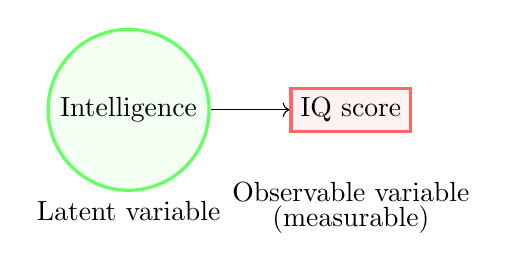
\begin{tikzpicture}[
  roundnode/.style={circle, draw=green!60, fill=green!5, very thick, minimum size=7mm},
  squarednode/.style={rectangle, draw=red!60, fill=red!5, very thick, minimum size=5mm},
]

% Nodes
\node[squarednode] (maintopic) {IQ score};
\node[roundnode] (intelligence) [left=of maintopic] {Intelligence};

% Text labels with positioning
\node [below=of intelligence, yshift=10mm] {Latent variable};
\node [below=of maintopic, yshift=5mm] {Observable variable};
\node [below=of maintopic, yshift=2mm] {(measurable)};

% Lines
\draw[->] (intelligence.east) -- (maintopic.west);

\end{tikzpicture}
\end{center}

This is why we must first measure or observe values $x$ (IQ score), so we can estimate $P(z|x)$ (intelligence). We know that the IQ score tests is Gaussian (normal) distributed with mean ($\mu$) of 100 with standard deviation ($\sigma$) of 15 points. We can say that $P(intelligence)$ is the prior distribution, because it represents our initial belief of possible values of intelligence. If we have little to no prior knowledge about intelligence, we can also assume its uniform distributed, similarly to IQ score.

The posterior distribution $P(intelligence|IQ)$ is the updated belief about the possible values of intelligence \textbf{after} we observed their IQ score. It takes into account the prior knowledge and the information from observed variables, such as IQ.


\subsection{Likelihood function}
\label{appendix:likelihood_function}

Likelihood function in the realm of generative models, is often used to capture the underlying data distribution (generate data points with similar likelihood to the training data distribution).

The formal notion of likelihood function is: $L(x | \theta)$, which reflects the probability of a specific data point ($x$) being generated by the model with its current parameters ($\theta$). We want to maximize this term: $\underset{\theta}{\arg\max}\ L(x | \theta)$. In many cases it's computationally more convenient to maximize the \textbf{log-likelihood} function instead, as the logarithm is a monotonic function (always increasing or decreasing, and therefor the log of the function is also monotonic):

\[
    \hat{\theta}_{MLE} = \underset{\theta}{\arg\max} \ \log L(\mathbf{x} | \theta)
\]

Since directly calculating the likelihood is often intractable, methods like \textbf{maximum likelihood estimation (MLE)} optimize $\theta$ indirectly. To address intractability, approaches such as \textbf{Evidence Lower Bound (ELBO)} are used as alternative loss functions. Additionally, adversarial training is widely employed in GAN-based models.

\subsection{Variational Inference (VI)}
\label{appendix:variational_inference}

Variational inference (VI) is a technique used to approximate complex posterior distributions in Bayesian inference. Instead of directly maximizing the log-likelihood function, VI aims to minimize the \textbf{Kullback-Leibler (KL) divergence} between an approximate posterior distribution and the true posterior distribution (for instance, learn the distribution of 2D points that are generated by the model, which is estimation of another distribution we want the model to learn, for instance, Gaussian). This is often achieved by minimizing a proxy loss function, such as the \textbf{Evidence Lower Bound (ELBO)}, which is tractable (can be effectively computed) to optimize. By minimizing the ELBO, VI effectively guides the approximate posterior distribution towards the true posterior distribution.
\subsection{Kullback-Leibler (KL) divergence}
\label{appendix:kl_divergence}

\begin{figure}
    \centering
    \caption{Showcase of KL-Divergence of three different normal distributions. The divergence between two normal distributions can occur in both mean and variance. Mean (or expectation) is the center of the distribution, while variance is the spread of the distribution.}
    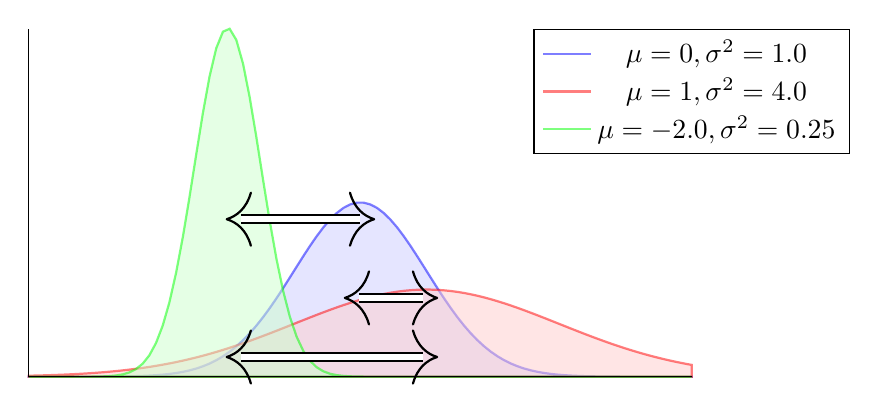
\begin{tikzpicture}
        \begin{axis} [
          no markers, 
          domain=-5:5, 
          samples=100,
          axis lines*=left, 
          height=6cm, 
          width=10cm,
          xtick=\empty, 
          ytick=\empty,
          enlargelimits=false, 
          clip=false, 
          axis on top,
          grid = major,
          legend style={at={(1,1)}, anchor=north, legend columns=1},
        ]

        % Define variables (mean, variance)
        \pgfmathsetmacro{\muA}{0}
        \pgfmathsetmacro{\sigmaA}{1}
        \pgfmathsetmacro{\varA}{\sigmaA^2}
        
        \pgfmathsetmacro{\muB}{1}
        \pgfmathsetmacro{\sigmaB}{2}
        \pgfmathsetmacro{\varB}{\sigmaB^2}
        
        \pgfmathsetmacro{\muC}{-2}
        \pgfmathsetmacro{\sigmaC}{0.5}
        \pgfmathsetmacro{\varC}{\sigmaC^2}
    
        % Blue
        \addplot[blue, thick, fill=blue!20, opacity=0.5] 
        {1/sqrt(2*pi*\sigmaA^2) * exp(-0.5 * ((x-\muA)/\sigmaA)^2)} \closedcycle;
        \addlegendentry{$\mu = \muA, \sigma^2 = \varA$};

        % Red
        \addplot[red, thick, fill=red!20, opacity=0.5] 
        {1/sqrt(2*pi*\sigmaB^2) * exp(-0.5 * ((x-\muB)/\sigmaB)^2)} \closedcycle;
        \addlegendentry{$\mu = \muB, \sigma^2 = \varB$};

        % Green
        \addplot[green, thick, fill=green!20, opacity=0.5] 
        {1/sqrt(2*pi*\sigmaC^2) * exp(-0.5 * ((x-\muC)/\sigmaC)^2)} \closedcycle;
        \addlegendentry{$\mu = \muC, \sigma^2 = \varC$};
        
        \end{axis}

        % Arrows between distributions
        % Blue, Green
        \draw[{<._[sep=-4pt]}-{_[sep=-4pt].>}, line width=0.8pt, double, double distance=2pt] (2.5,2) -- (4.4,2);
        % Green, Red
        \draw[{<._[sep=-4pt]}-{_[sep=-4pt].>}, line width=0.8pt, double, double distance=2pt] (2.5,0.25) -- (5.2,0.25);
        % Blue, Red
        \draw[{<._[sep=-4pt]}-{_[sep=-4pt].>}, line width=0.8pt, double, double distance=2pt] (4,1) -- (5.2,1);

    \end{tikzpicture}
    \label{fig:kl_divergence}
\end{figure}

Kullback-Leibler (KL) divergence allows us to measure the difference between two probability distributions, $P$ and $Q$. It essentially quantifies how much information is lost when using distribution $Q$ to approximate distribution $P$.

In various applications, we deal with situations where we have a true underlying distribution (P) representing the actual data generation process, but we might not know its exact form. We might have another distribution (Q), perhaps a model we've built, that we want to use to represent or approximate the true distribution. KL divergence helps us understand how well Q captures the information present in P. In other words, \textbf{how much diverged the distribution Q is from the distribution P}. See figure \ref{fig:kl_divergence} for a visual representation.

The mathematical formula for KL-divergence is:

\begin{equation}
\label{eq:kl-divergence}
    D_{KL}(P || Q) = \sum_{x \in X} P(x) \cdot log(\frac{P(x)}{Q(x)})
\end{equation}

where $x \in X$ represents all the possible values within the data space ($X$).

A KL-divergence value of 0 indicate that the distribution $Q$ perfectly captures the distribution $P$, and larger numbers indicate higher disparity.

KL-divergence measures information lost, so if both $P,Q$ are Gaussian distributions with the same mean and standard deviation, we have no information lost. But if the standard deviation or the mean is different, KL-divergence measures that. On the other hand, directly integrating the distributions and measuring the area under the curve (AUC) will not show information loss if the standard deviation is the same, but the mean is different.


Other notations are used as well: $p_\theta(x_i), q_\phi(x_i)$. Most of the time we are dealing with small numbers in the probabilities, which will get multiplied with other small numbers, which may result in rounding to zero. So instead we generally compute \textbf{log-likelihood}: $log\ p_\theta(x_i), log\ q_\phi(x_i)$. Now to compare two distributions we can compute the difference: $log\ p_\theta(x_i) - log\ q_\phi(x_i)$ and if that subtraction result in zero that means that our approximated distribution $q$ is identical to ground truth $p$. We can rewrite it like so: 

\begin{equation}
\label{eq:log-likelihood}
    log\ [\frac{p_\theta(x_i)}{q_\phi(x_i)}]
\end{equation}

which is also sometimes called \textbf{log-likelihood ratio}.

In reality, we are only interested in the \textbf{average difference} between $p_\theta$ and $q_\phi$. Because we are dealing with random variables $x \in X$, instead of average we say \textbf{expected value} of a random variable. Weighted average of instances of random variables is:

\begin{equation*}
    \mathbb{E}_{p_\theta} [X] = \sum_{i=1}^{\infty} x_i p_\theta(x_i)
\end{equation*}

where $x_i$ is the state of the random variable, and $p_\theta(x_i)$ is the weight (weight of contribution to the average). A more general formulation is given by:

\begin{equation*}
    \mathbb{E}_{p_\theta} [h(X)] = \sum_{i=1}^{\infty} h(x_i) p_\theta(x_i)
\end{equation*}

where $h(X), h(x_i)$ is a function of random variable $x_i \in X$. This formulation works for discrete random variable, here is the formulation for continuous random variable:

\begin{equation*}
    \mathbb{E}_{p_\theta} [h(X)] = \int_{\mathbb{R}} h(x) p_\theta(x) dx
\end{equation*}

Let's get back to the average likelihood (equation \ref{eq:log-likelihood}), we can set $h(X) = log\ [\frac{p_\theta(x_i)}{q_\phi(x_i)}]$, and we get:

\begin{equation*}
    \sum_{i=1}^{\infty} p_\theta(x_i) log\ [\frac{p_\theta(x_i)}{q_\phi(x_i)}]
\end{equation*}

where $p_\theta(x_i)$ is the weight. This equation is called the \textbf{KL-divergence}:

\begin{equation}
\label{eq:kl_divergence}
    \mathbb{E}_p [log\ \frac{p_\theta(x_i)}{q_\phi(x_i)}]
    =
    \sum_{i=1}^{\infty} p_\theta(x_i) log\ [\frac{p_\theta(x_i)}{q_\phi(x_i)}]
    =
    D_{KL} (p_\theta || q_\phi)
\end{equation}

In short, this is the expected value of the log-likelihood ratio (of discrete random variable). For continuous random variable we get similar formula:

\begin{equation}
\label{eq:kl_divergence_continous}
    \mathbb{E}_p [log\ \frac{p_\theta(x_i)}{q_\phi(x_i)}]
    =
    \int_{\mathbb{R}} p_\theta(x) log\ [\frac{p_\theta(x)}{q_\phi(x)}] dx
    =
    D_{KL} (p_\theta || q_\phi)
\end{equation}

One problem we are dealing with is the infinity space in both equations.  To get around it, we can use the \textbf{law of large numbers} which says:

\begin{equation*}
    \frac{1}{N} \sum_{i=1}^N h(x_i) \approx \mathbb{E}_p [h(X)]
\end{equation*}

and we get:

\begin{equation}
    D_{KL} (p_\theta || q_\phi) \approx
    \frac{1}{N} \sum_{i=1}^N log\ [\frac{p_\theta(x_i)}{q_\phi(x_i)}]
\end{equation}

Credit to \cite{dk-divergence-math-explanation} for the math explanation.
\subsection{Evidence Lower Bound (ELBO)}
\label{appendix:elbo}

Evidence Lower Bound (ELBO) provides an efficient way to optimize and train models that are based on variational inference (often called latent models), like VAEs or GANs. ELBO is an estimation for the log-likelihood function, and since the likelihood function is intractable in latent models (that use latent variables $z$) to calculate directly, ELBO is used instead as approximation (its tractable). ELBO achieves this by setting a lower bound on the likelihood of observing data $x$. By maximizing ELBO we essentially optimize the model by maximizing likelihood.

As we saw in equation \ref{eq:vae_posterior} the likelihood function we want to optimize is:

\begin{equation}
    p(x) = \int p(x | z) \cdot p(z) dz
\end{equation}

where $p(x)$ is the likelihood of observing data $x$, $p(x | z)$ is probability of reconstructing $x$ given latent variable $z$,  $p(z)$ is the prior distribution of latent variable $z$, and the integral is over all possible values of $z$ (if $z$ is discrete, the integral is replaced by a sum).

The reason this integral is intractable is because it is computationally expensive to calculate the likelihood of all possible values of $z$. To solve this, we can use ELBO (also defined at equation \ref{eq:vae_elbo}), which is defined as:

\begin{equation}
    \text{ELBO} = \mathbb{E}_z[\log p(x | z)] - KL(q(z) \Vert p(z))
    \label{eq:elbo}
\end{equation}

where $\mathbb{E}_z[\log p(x | z)]$ is the expected reconstruction loss, and $KL(q(z) \Vert p(z))$ is the Kullback-Leibler divergence (see appendix \ref{appendix:kl_divergence}) between the approximate posterior $q(z)$ and the prior distribution $p(z)$.

The reason this is tractable is because we use mean (expectation) instead of integrating, and both the reconstruction loss and KL divergence are well defined and tractable. 

\subsection{VQ-VAE}

In listing \ref{lst:vq_codebook} we can see that the researchers divided the code vectors by number of embeddings, which normalizes the vectors in order to stabilize the training (the codebook vectors will have unit variance).

\begin{lstlisting}[language=Python, label=lst:vq_codebook, caption=Code of the quantisizer module of VQ-VAE paper. Shows the initialization of the codebook vectors.]
    class VectorQuantizer(nn.Module):
    """
    Discretization bottleneck part of the VQ-VAE.

    Inputs:
    - n_e : number of embeddings
    - e_dim : dimension of embedding
    - beta : commitment cost used in loss term, beta * ||z_e(x)-sg[e]||^2
    """

    def __init__(self, n_e, e_dim, beta):
        super(VectorQuantizer, self).__init__()
        self.n_e = n_e
        self.e_dim = e_dim
        self.beta = beta

        self.embedding = nn.Embedding(self.n_e, self.e_dim)
        self.embedding.weight.data.uniform_(-1.0 / self.n_e, 1.0 / self.n_e)
\end{lstlisting}




\begin{lstlisting}[language=Python, label=lst:vqvae_distance, caption=Euclidean distance calculation in VQ-VAE paper between embedding and codebook vectors $\Vert z-e \Vert$.]

    def forward(self, z):
        """
        Inputs the output of the encoder network z and maps it to a discrete 
        one-hot vector that is the index of the closest embedding vector e_j

        z (continuous) -> z_q (discrete)

        z.shape = (batch, channel, height, width)

        quantization pipeline:

            1. get encoder input (B,C,H,W)
            2. flatten input to (B*H*W,C)

        """
        # reshape z -> (batch, height, width, channel) and flatten
        z = z.permute(0, 2, 3, 1).contiguous()
        z_flattened = z.view(-1, self.e_dim)
        # distances from z to embeddings e_j (z - e)^2 = z^2 + e^2 - 2 e * z

        d = torch.sum(z_flattened ** 2, dim=1, keepdim=True) + \
            torch.sum(self.embedding.weight**2, dim=1) - 2 * \
            torch.matmul(z_flattened, self.embedding.weight.t())
    
\end{lstlisting}


\begin{lstlisting}[language=Python, label=lst:vqvae_loss, caption=Loss function as defined in the VQ-VAE paper (eq. \ref{eq:vq_loss}). The detach keyword is the stop gradient operation.]
    # compute loss for embedding
    loss = torch.mean((z_q.detach()-z)**2) + self.beta * \
        torch.mean((z_q - z.detach()) ** 2)
\end{lstlisting}



\begin{lstlisting}[language=Python, label=lst:vqvae_stop_gradients, caption=Allow gradients to flow through the snapping operation.]
    # preserve gradients
    z_q = z + (z_q - z).detach()
\end{lstlisting}
\subsection{Transformers}
\label{appendix:transformers}

...

\end{document}